\documentclass[12pt]{extarticle}
\usepackage[paperwidth=15in,paperheight=7.2in]{geometry}
\usepackage{amsmath}
\usepackage{hyperref}
\usepackage{multirow}
\usepackage{pdfpages}
\usepackage[utf8]{inputenc}
\title{Kaon mixing: chiral and continuum extrapolations}
\author{R Mukherjee}
\date{\today}
\begin{document}
\maketitle
\tableofcontents
\clearpage
\begin{figure}
\centering
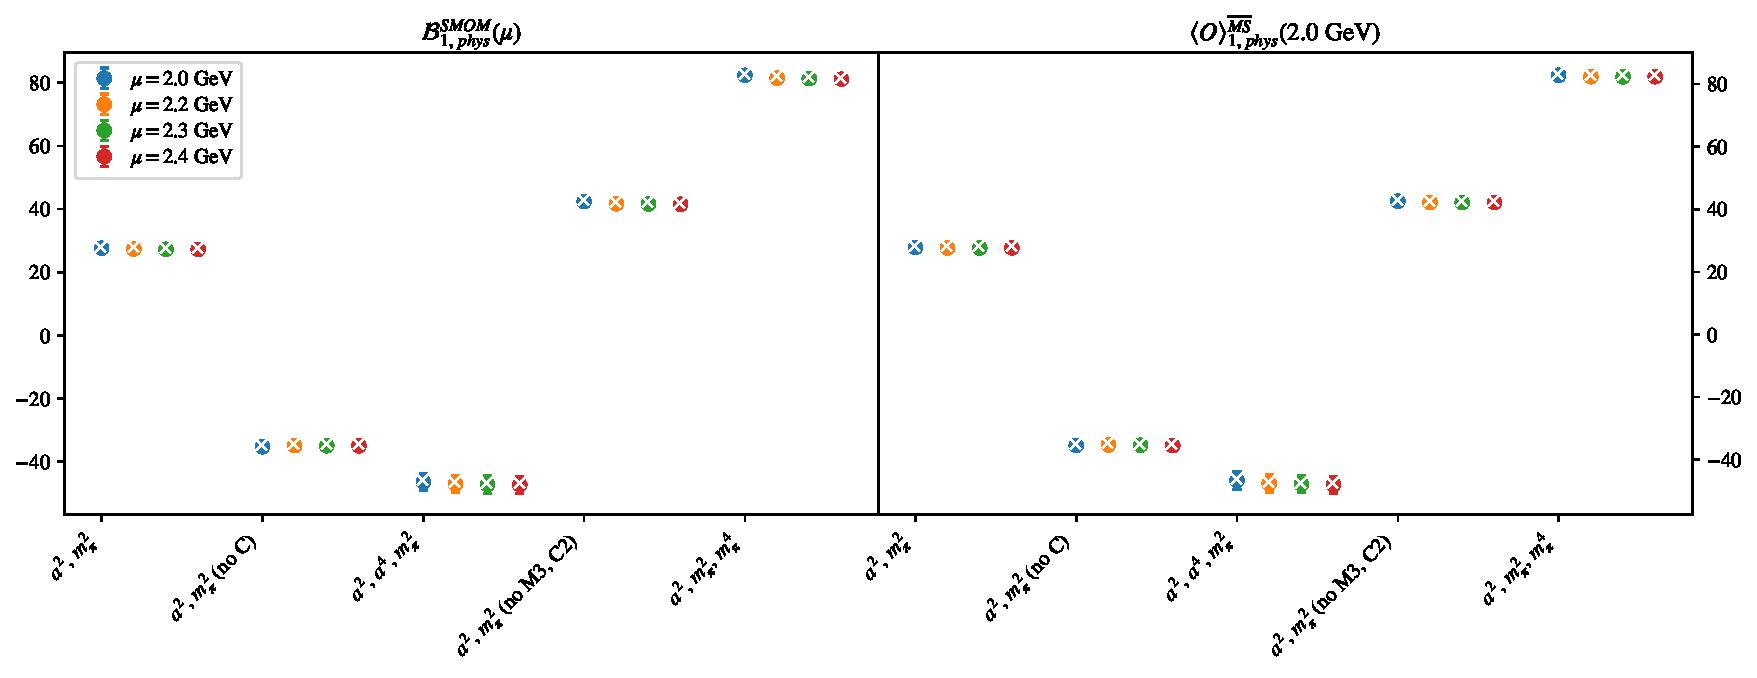
\includegraphics[page=1, width=1.1\textwidth]{VVpAA/NPR/fit_summary_fq_op.pdf}
\caption{$\langle O \rangle_{1}$\\(left) $\langle O \rangle_{phys}$ in RI/SMOM scheme from fit variations (fits with $p$-value $<0.05$ marked with ``$\times$"). \\(right) $\langle O \rangle_{phys}$ in $\overline{MS}$ computed using $\langle O \rangle^{\overline{MS}} = R^{\overline{MS}\leftarrow SMOM}(2.0)\sigma_{npt}(2.0,\mu) \langle O \rangle^{SMOM}(\mu)$.}
\end{figure}
\clearpage
\begin{figure}
\centering
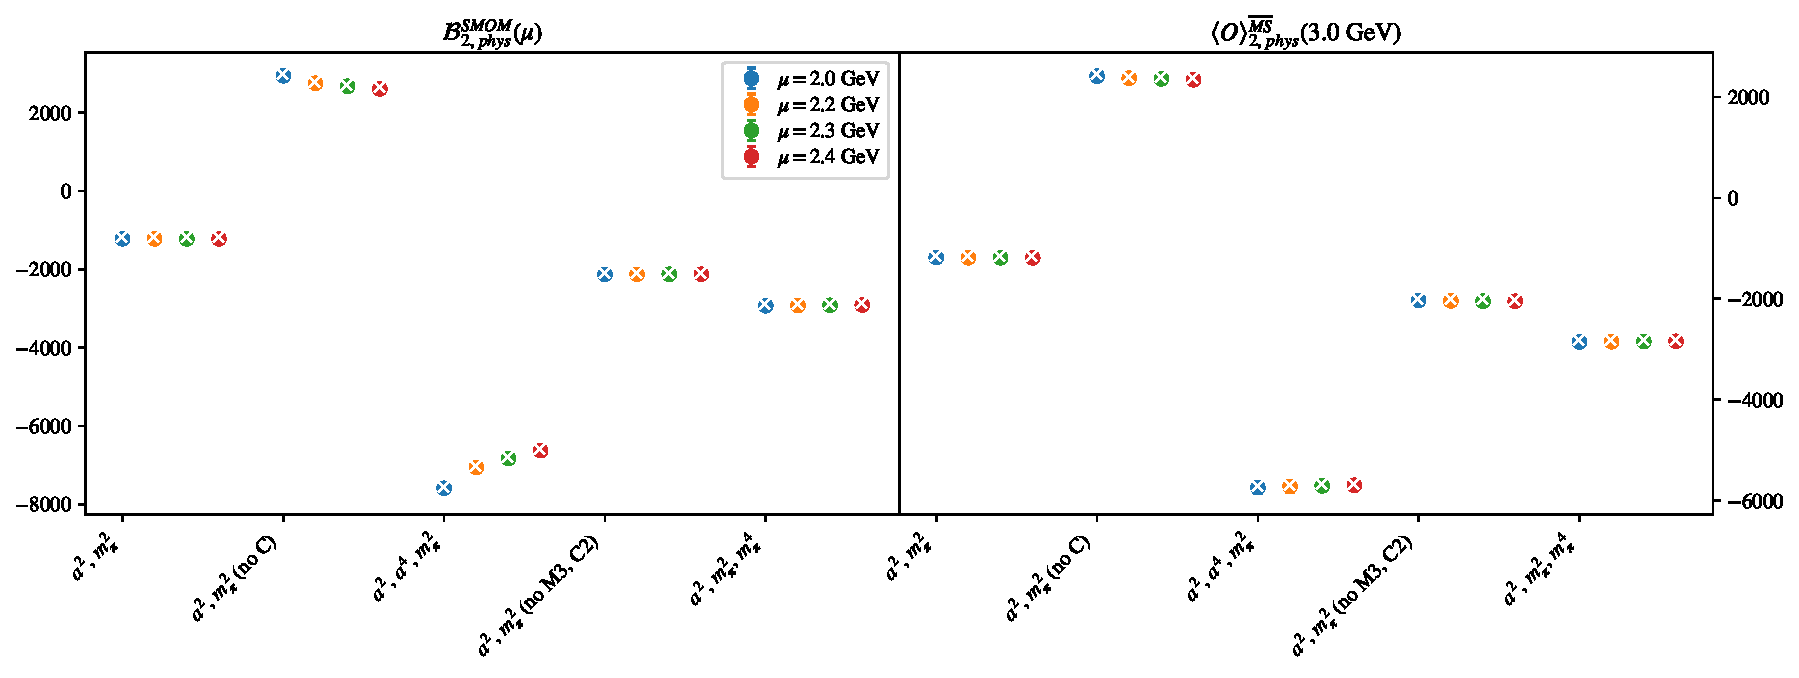
\includegraphics[page=1, width=1.1\textwidth]{VVmAA/NPR/fit_summary_fq_op.pdf}
\caption{$\langle O \rangle_{2}$\\(left) $\langle O \rangle_{phys}$ in RI/SMOM scheme from fit variations (fits with $p$-value $<0.05$ marked with ``$\times$"). \\(right) $\langle O \rangle_{phys}$ in $\overline{MS}$ computed using $\langle O \rangle^{\overline{MS}} = R^{\overline{MS}\leftarrow SMOM}(3.0)\sigma_{npt}(3.0,\mu) \langle O \rangle^{SMOM}(\mu)$.}
\end{figure}
\clearpage
\begin{figure}
\centering
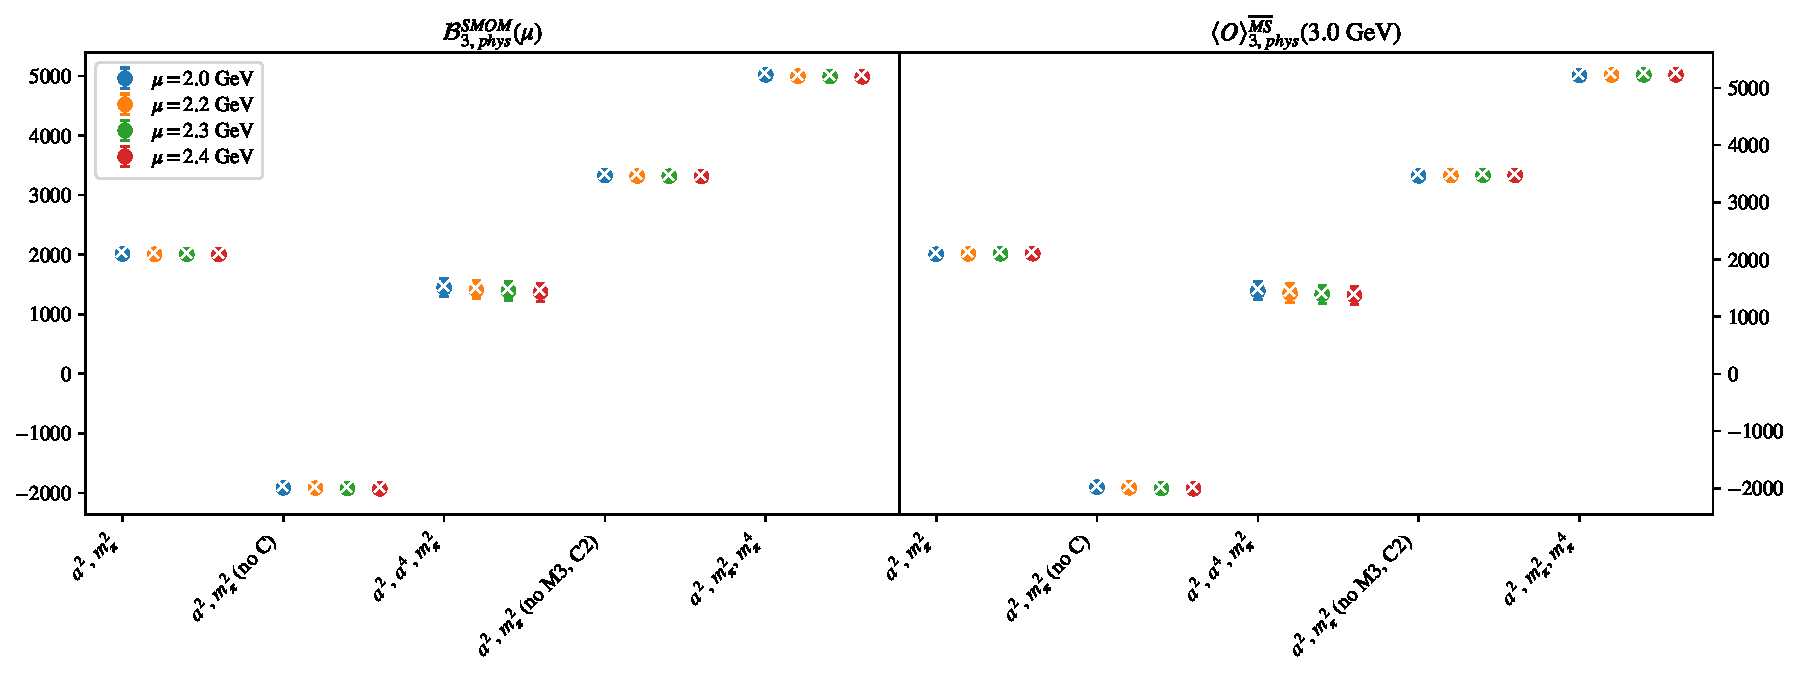
\includegraphics[page=1, width=1.1\textwidth]{SSmPP/NPR/fit_summary_fq_op.pdf}
\caption{$\langle O \rangle_{3}$\\(left) $\langle O \rangle_{phys}$ in RI/SMOM scheme from fit variations (fits with $p$-value $<0.05$ marked with ``$\times$"). \\(right) $\langle O \rangle_{phys}$ in $\overline{MS}$ computed using $\langle O \rangle^{\overline{MS}} = R^{\overline{MS}\leftarrow SMOM}(3.0)\sigma_{npt}(3.0,\mu) \langle O \rangle^{SMOM}(\mu)$.}
\end{figure}
\clearpage
\begin{figure}
\centering
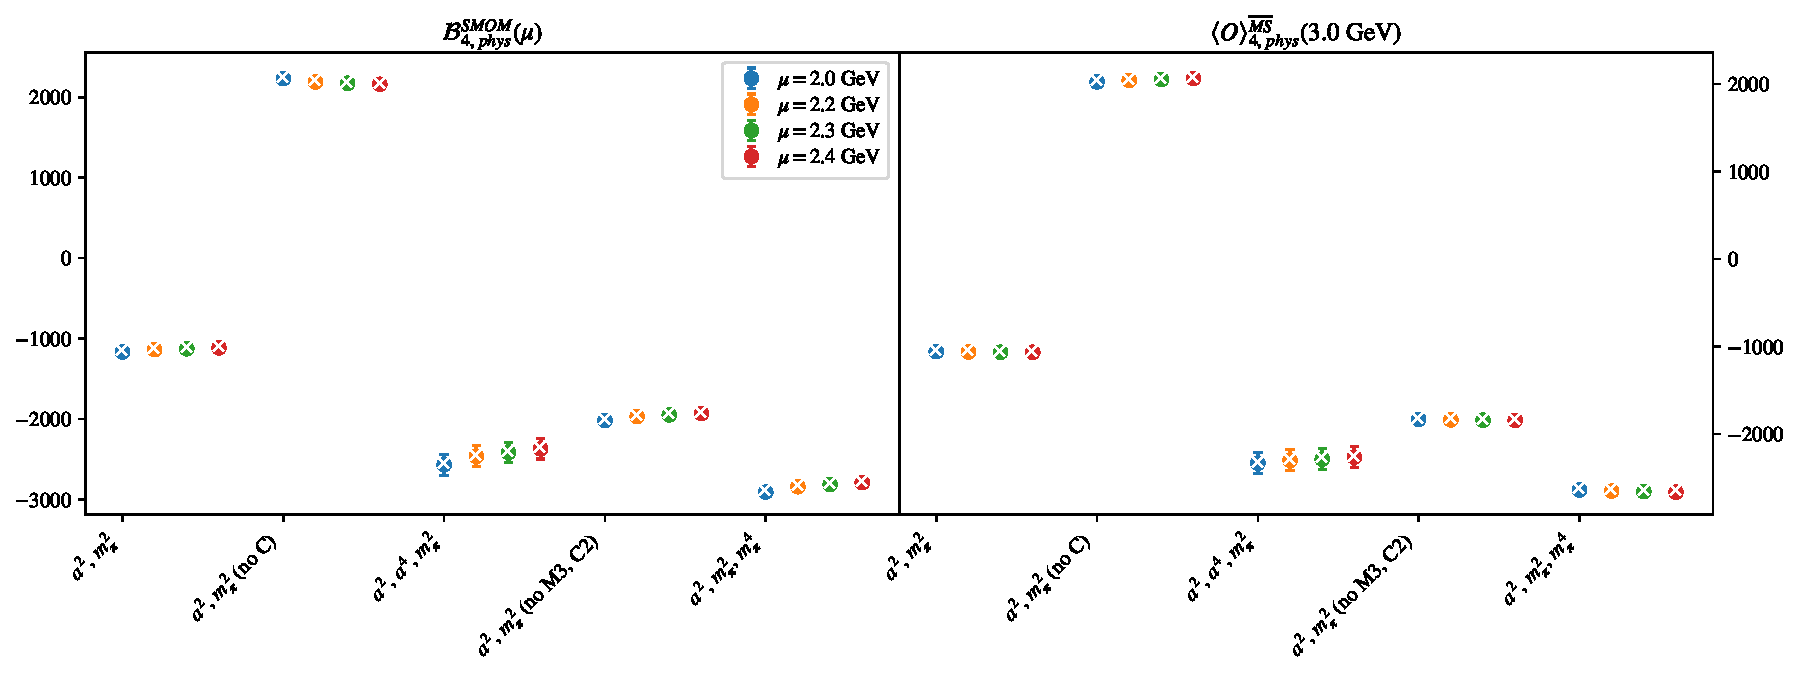
\includegraphics[page=1, width=1.1\textwidth]{SSpPP/NPR/fit_summary_fq_op.pdf}
\caption{$\langle O \rangle_{4}$\\(left) $\langle O \rangle_{phys}$ in RI/SMOM scheme from fit variations (fits with $p$-value $<0.05$ marked with ``$\times$"). \\(right) $\langle O \rangle_{phys}$ in $\overline{MS}$ computed using $\langle O \rangle^{\overline{MS}} = R^{\overline{MS}\leftarrow SMOM}(3.0)\sigma_{npt}(3.0,\mu) \langle O \rangle^{SMOM}(\mu)$.}
\end{figure}
\clearpage
\begin{figure}
\centering
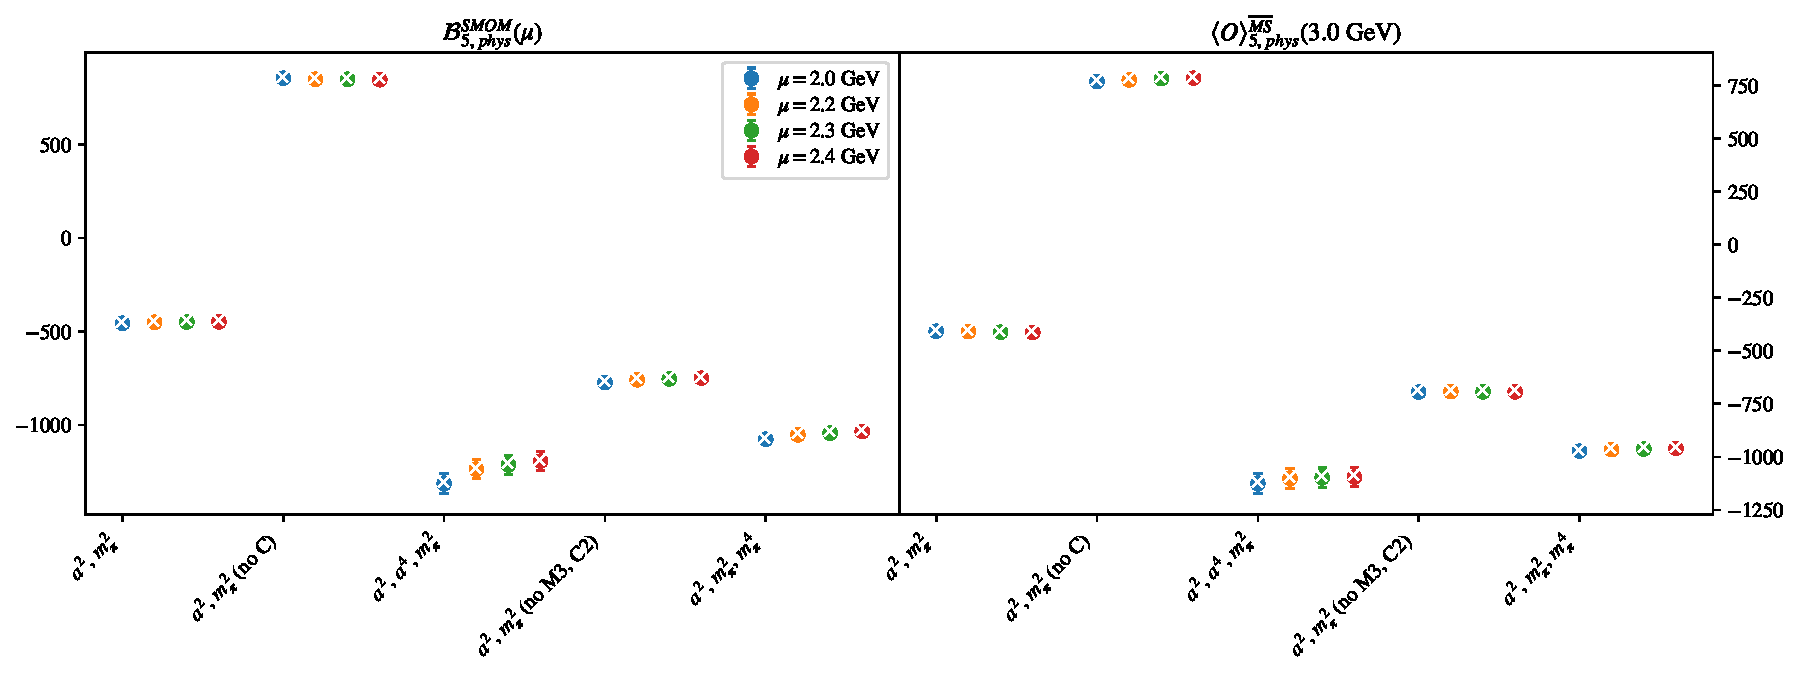
\includegraphics[page=1, width=1.1\textwidth]{TT/NPR/fit_summary_fq_op.pdf}
\caption{$\langle O \rangle_{5}$\\(left) $\langle O \rangle_{phys}$ in RI/SMOM scheme from fit variations (fits with $p$-value $<0.05$ marked with ``$\times$"). \\(right) $\langle O \rangle_{phys}$ in $\overline{MS}$ computed using $\langle O \rangle^{\overline{MS}} = R^{\overline{MS}\leftarrow SMOM}(3.0)\sigma_{npt}(3.0,\mu) \langle O \rangle^{SMOM}(\mu)$.}
\end{figure}
\clearpage
\section{$\mathcal{B}_1$}
\begin{table}[h!]
\begin{center}
\begin{tabular}{|c|c|c|c|c|c|}
\hline
$\mu$ (GeV) & $a^2$, $m_\pi^2$& $a^2$, $m_\pi^2$ (no C)& $a^2$, $a^4$, $m_\pi^2$& $a^2$, $m_\pi^2$ (no M3, C2)& $a^2$, $m_\pi^2$, $m_\pi^4$\\
\hline
2.0& \hyperlink{VVpAA/NPR/a2m2_20.pdf.1}{\textbf{27.6(37)}: 31395.801 (0.0)} & \hyperlink{VVpAA/NPR/a2m2noC_20.pdf.1}{\textbf{-35(14)}: 38933.302 (0.0)} & \hyperlink{VVpAA/NPR/a2a4m2_20.pdf.1}{\textbf{-46(27)}: 38585.869 (0.0)} & \hyperlink{VVpAA/NPR/a2m2mcut_20.pdf.1}{\textbf{42.3(64)}: 33587.411 (0.0)} & \hyperlink{VVpAA/NPR/a2m2m4_20.pdf.1}{\textbf{82.3(60)}: 14300.65 (0.0)}\\
2.2& \hyperlink{VVpAA/NPR/a2m2_22.pdf.1}{\textbf{27.3(36)}: 31608.024 (0.0)} & \hyperlink{VVpAA/NPR/a2m2noC_22.pdf.1}{\textbf{-34(14)}: 39223.15 (0.0)} & \hyperlink{VVpAA/NPR/a2a4m2_22.pdf.1}{\textbf{-47(27)}: 38821.954 (0.0)} & \hyperlink{VVpAA/NPR/a2m2mcut_22.pdf.1}{\textbf{41.6(63)}: 33975.784 (0.0)} & \hyperlink{VVpAA/NPR/a2m2m4_22.pdf.1}{\textbf{81.4(60)}: 14505.621 (0.0)}\\
2.3& \hyperlink{VVpAA/NPR/a2m2_23.pdf.1}{\textbf{27.2(36)}: 31654.959 (0.0)} & \hyperlink{VVpAA/NPR/a2m2noC_23.pdf.1}{\textbf{-34(14)}: 39280.306 (0.0)} & \hyperlink{VVpAA/NPR/a2a4m2_23.pdf.1}{\textbf{-47(27)}: 38875.092 (0.0)} & \hyperlink{VVpAA/NPR/a2m2mcut_23.pdf.1}{\textbf{41.5(63)}: 34030.531 (0.0)} & \hyperlink{VVpAA/NPR/a2m2m4_23.pdf.1}{\textbf{81.2(59)}: 14528.355 (0.0)}\\
2.4& \hyperlink{VVpAA/NPR/a2m2_24.pdf.1}{\textbf{27.2(36)}: 31677.595 (0.0)} & \hyperlink{VVpAA/NPR/a2m2noC_24.pdf.1}{\textbf{-34(14)}: 39318.403 (0.0)} & \hyperlink{VVpAA/NPR/a2a4m2_24.pdf.1}{\textbf{-47(27)}: 38899.494 (0.0)} & \hyperlink{VVpAA/NPR/a2m2mcut_24.pdf.1}{\textbf{41.5(62)}: 34047.877 (0.0)} & \hyperlink{VVpAA/NPR/a2m2m4_24.pdf.1}{\textbf{81.1(59)}: 14530.926 (0.0)}\\
\hline
\end{tabular}
\caption{Physical point value from chiral and continuum extrapolation at renormalisation scale $\mu$. Entries are \textbf{value(error)}: $\chi^2/\text{DOF}$ ($p$-value).}
\end{center}
\end{table}
\begin{table}[h!]
\begin{center}
\begin{tabular}{|c c|c|c|c|c|c|}
\hline
$\mu$ (GeV) &  & $a^2$, $m_\pi^2$& $a^2$, $m_\pi^2$ (no C)& $a^2$, $a^4$, $m_\pi^2$& $a^2$, $m_\pi^2$ (no M3, C2)& $a^2$, $m_\pi^2$, $m_\pi^4$\\
\hline
\multirow{2}{0.5in}{2.0} & $\alpha$ & 7.57(16)& -17.(39)& -19.(58)& 5.95(15)& 2.052(34)\\
 & $\beta$ & -0.228(35)& 0.1917(62)& 0.1507(79)& -0.301(50)& -0.436(25)\\
\hline
\multirow{2}{0.5in}{2.2} & $\alpha$ & 7.61(16)& -17.(39)& -19.(56)& 6.03(15)& 2.073(35)\\
 & $\beta$ & -0.229(35)& 0.1924(63)& 0.1476(75)& -0.303(51)& -0.437(25)\\
\hline
\multirow{2}{0.5in}{2.3} & $\alpha$ & 7.62(16)& -17.(39)& -19.(55)& 6.04(15)& 2.076(35)\\
 & $\beta$ & -0.229(35)& 0.1921(62)& 0.1471(75)& -0.303(51)& -0.438(25)\\
\hline
\multirow{2}{0.5in}{2.4} & $\alpha$ & 7.62(16)& -17.(39)& -19.(55)& 6.04(15)& 2.076(35)\\
 & $\beta$ & -0.229(35)& 0.1917(62)& 0.1466(74)& -0.303(51)& -0.438(25)\\
\hline
\end{tabular}
\caption{Fit values of coefficients in $Q = Q_{phys} + \mathbf{\alpha} a^2 + \mathbf{\beta}\left(\frac{m_\pi^2}{f_\pi^2}-\frac{m_{\pi,PDG}^2}{f_\pi^2}\right) + \ldots$.}
\end{center}
\end{table}
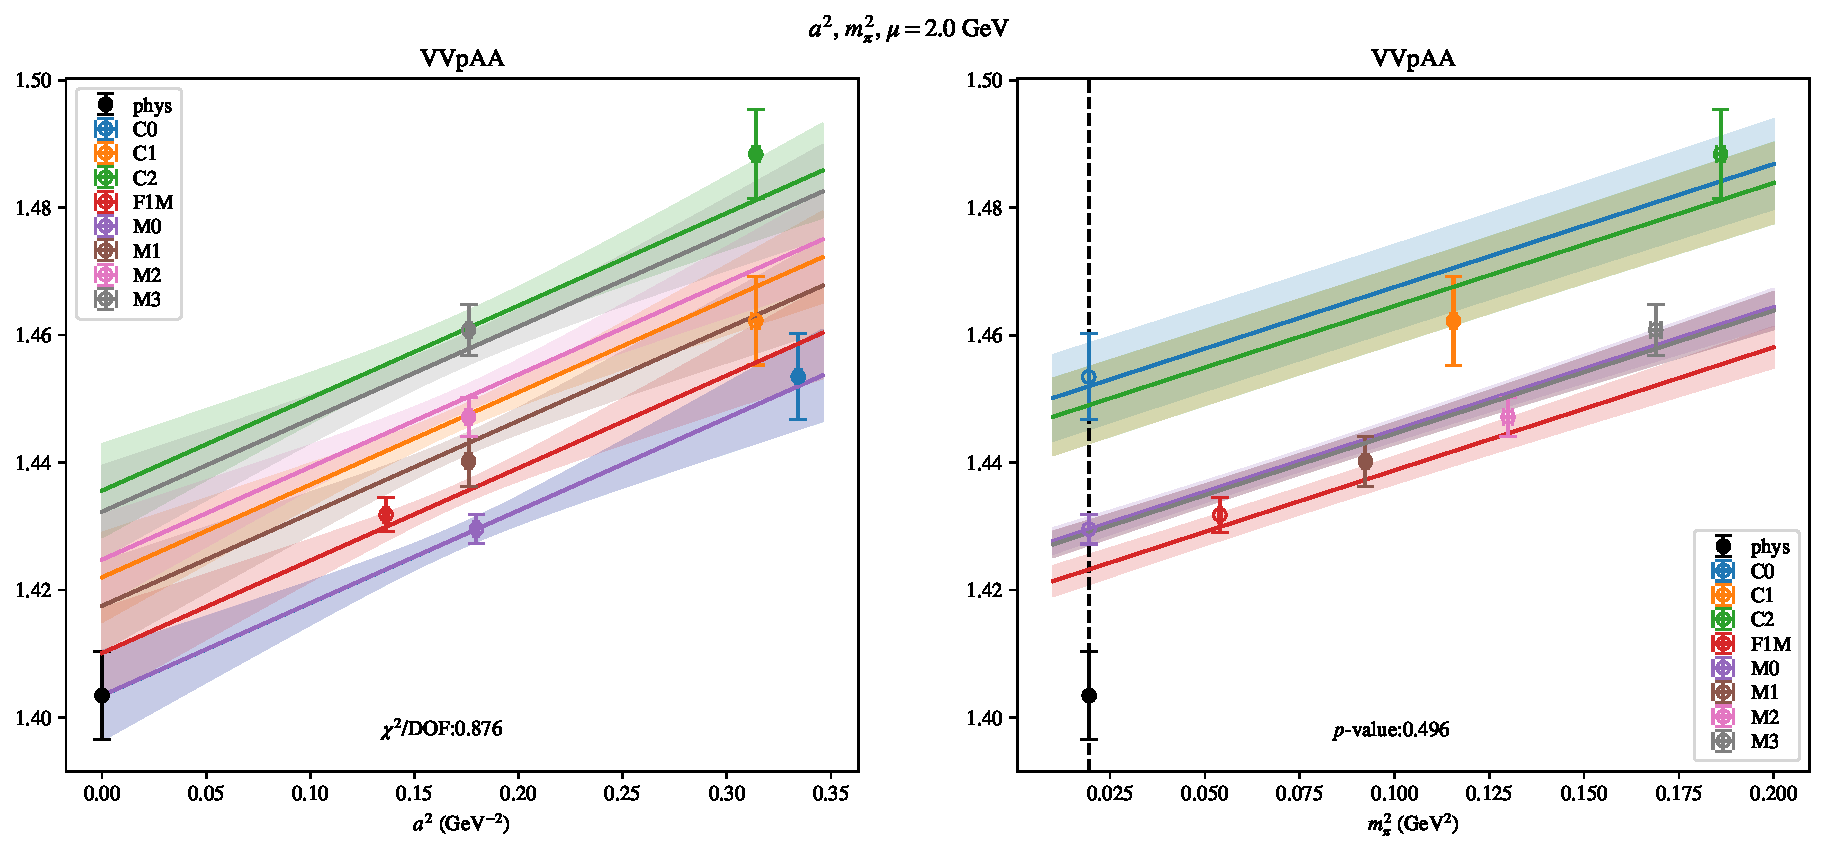
\includepdf[link, pages=-]{VVpAA/NPR/a2m2_20.pdf}
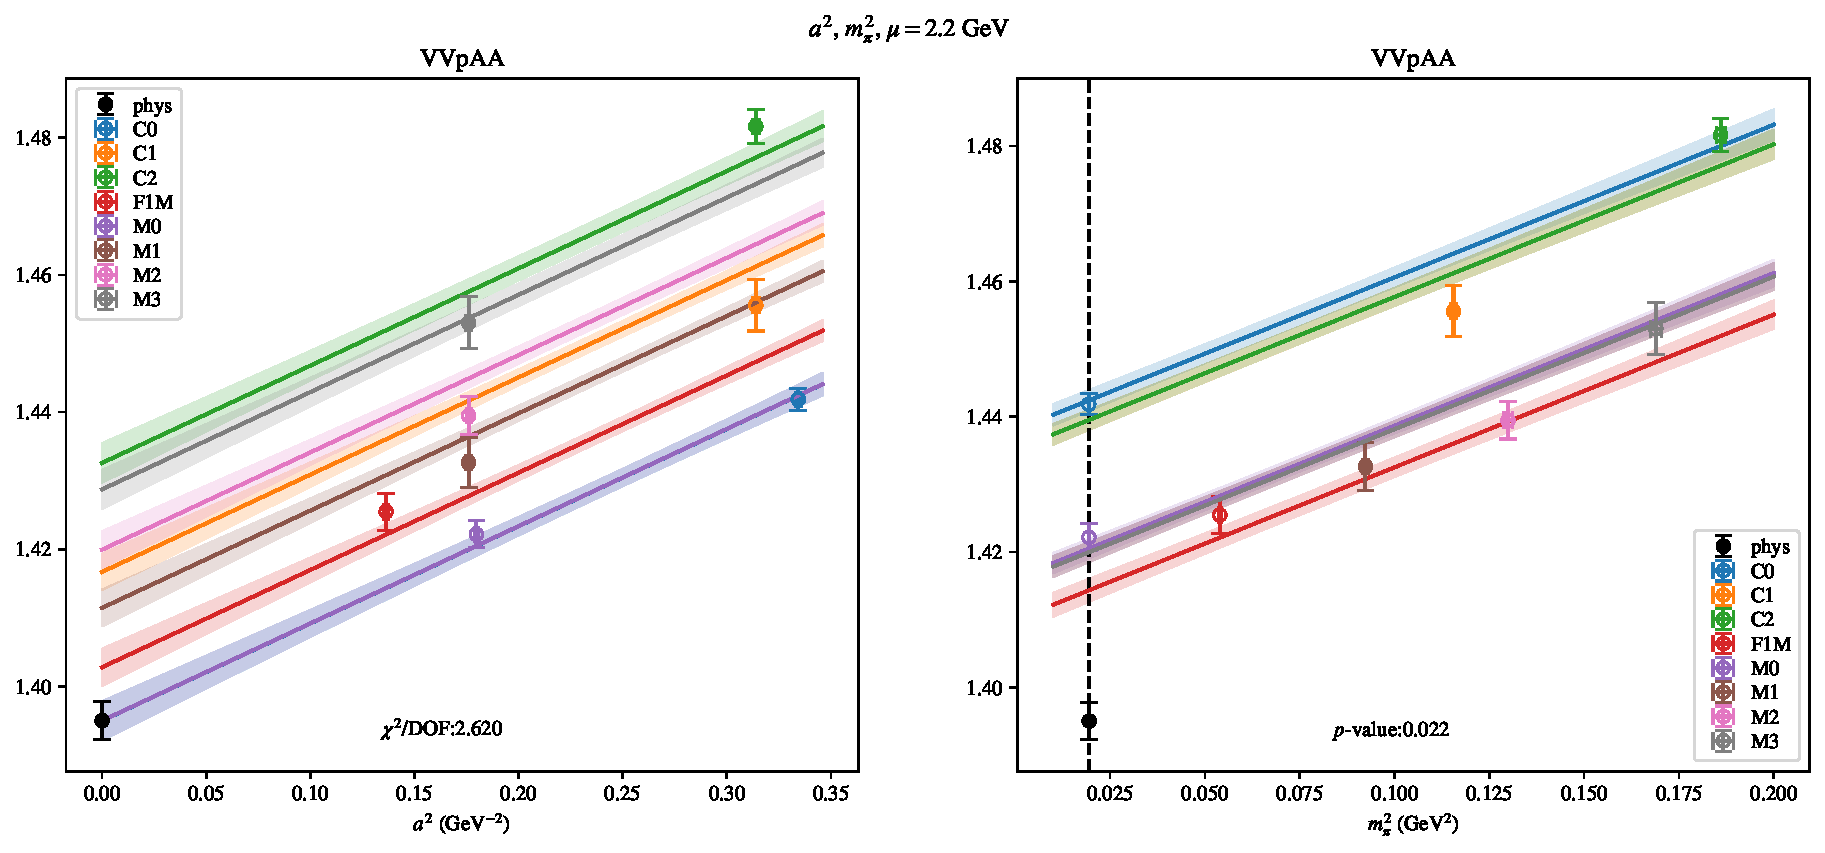
\includepdf[link, pages=-]{VVpAA/NPR/a2m2_22.pdf}
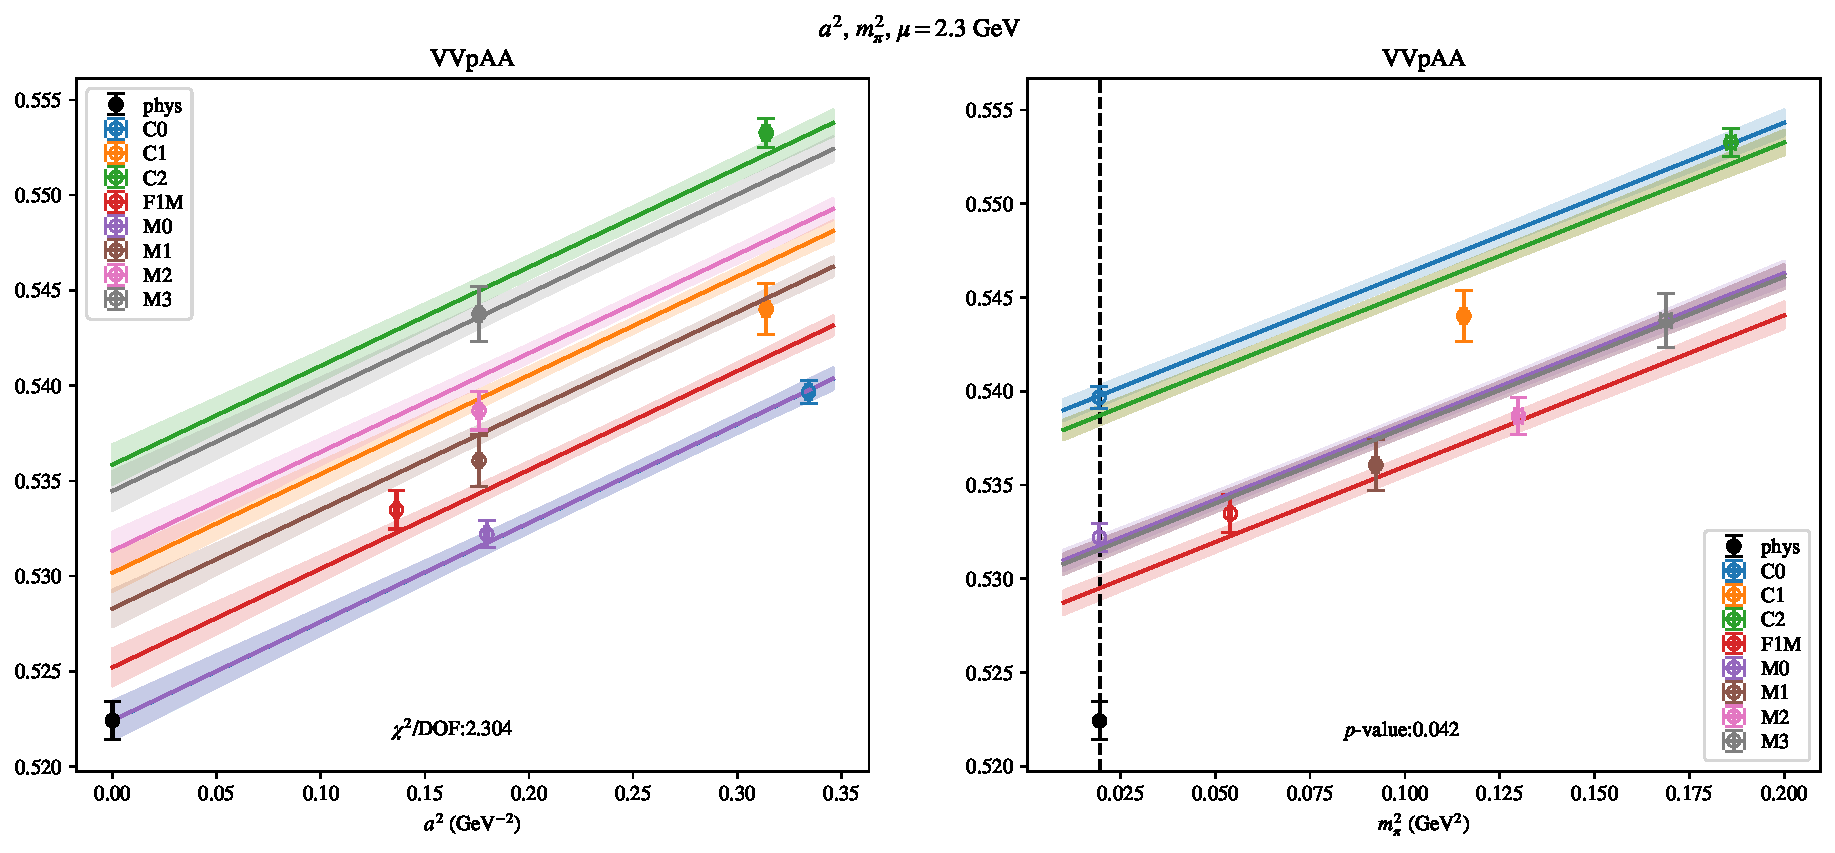
\includepdf[link, pages=-]{VVpAA/NPR/a2m2_23.pdf}
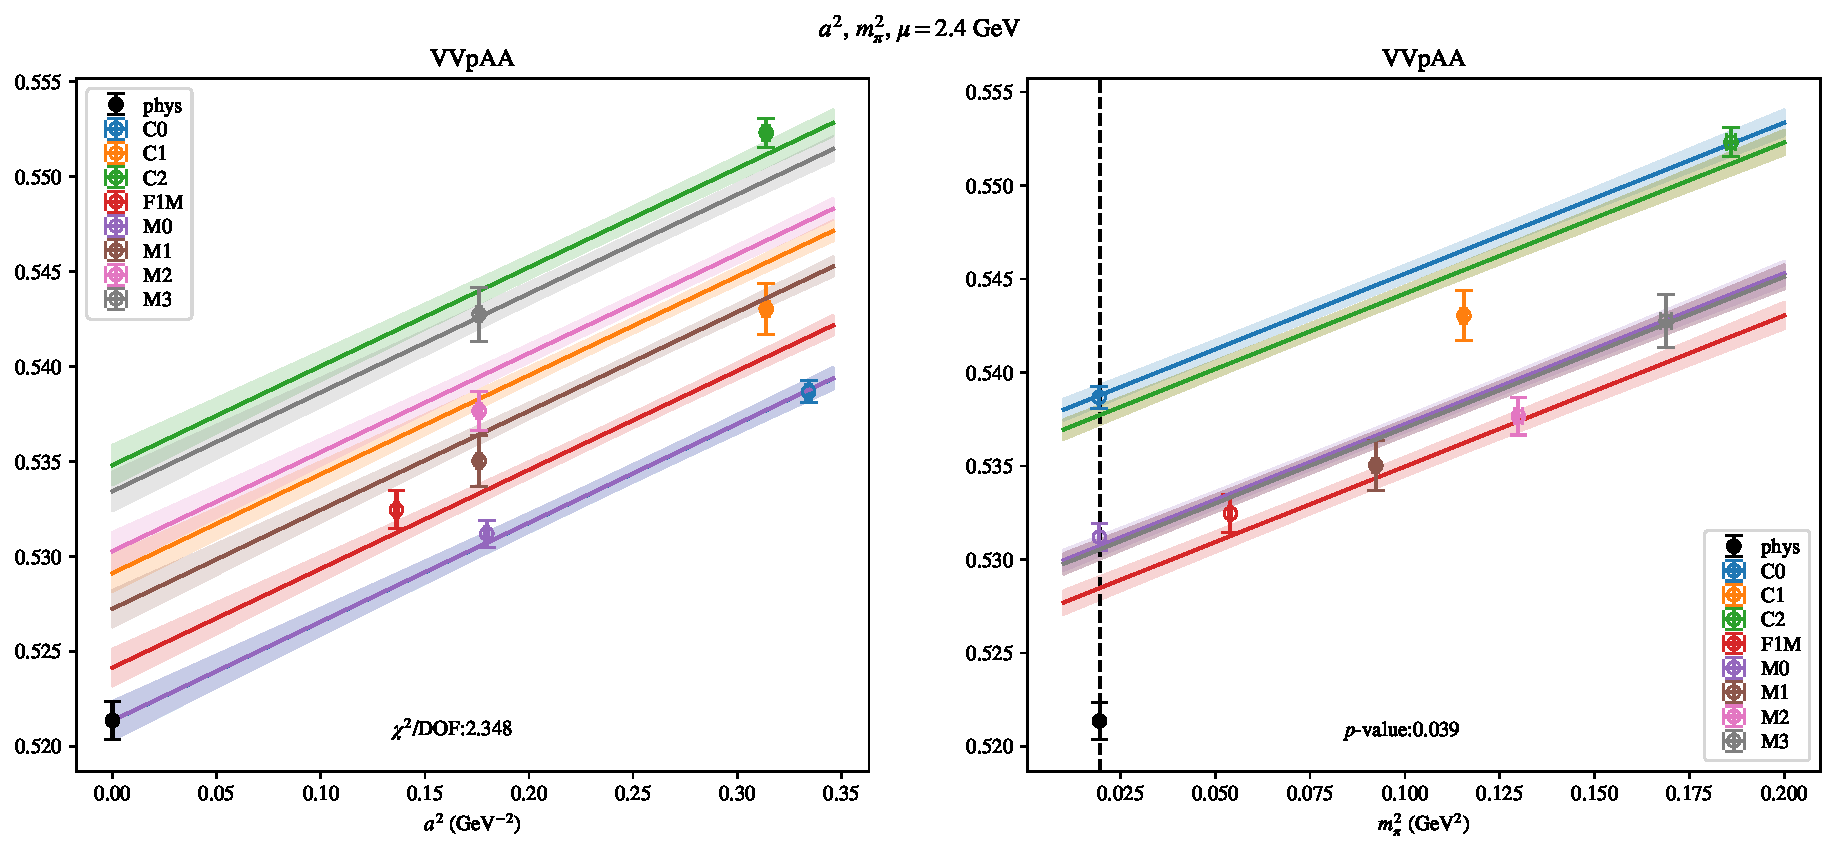
\includepdf[link, pages=-]{VVpAA/NPR/a2m2_24.pdf}
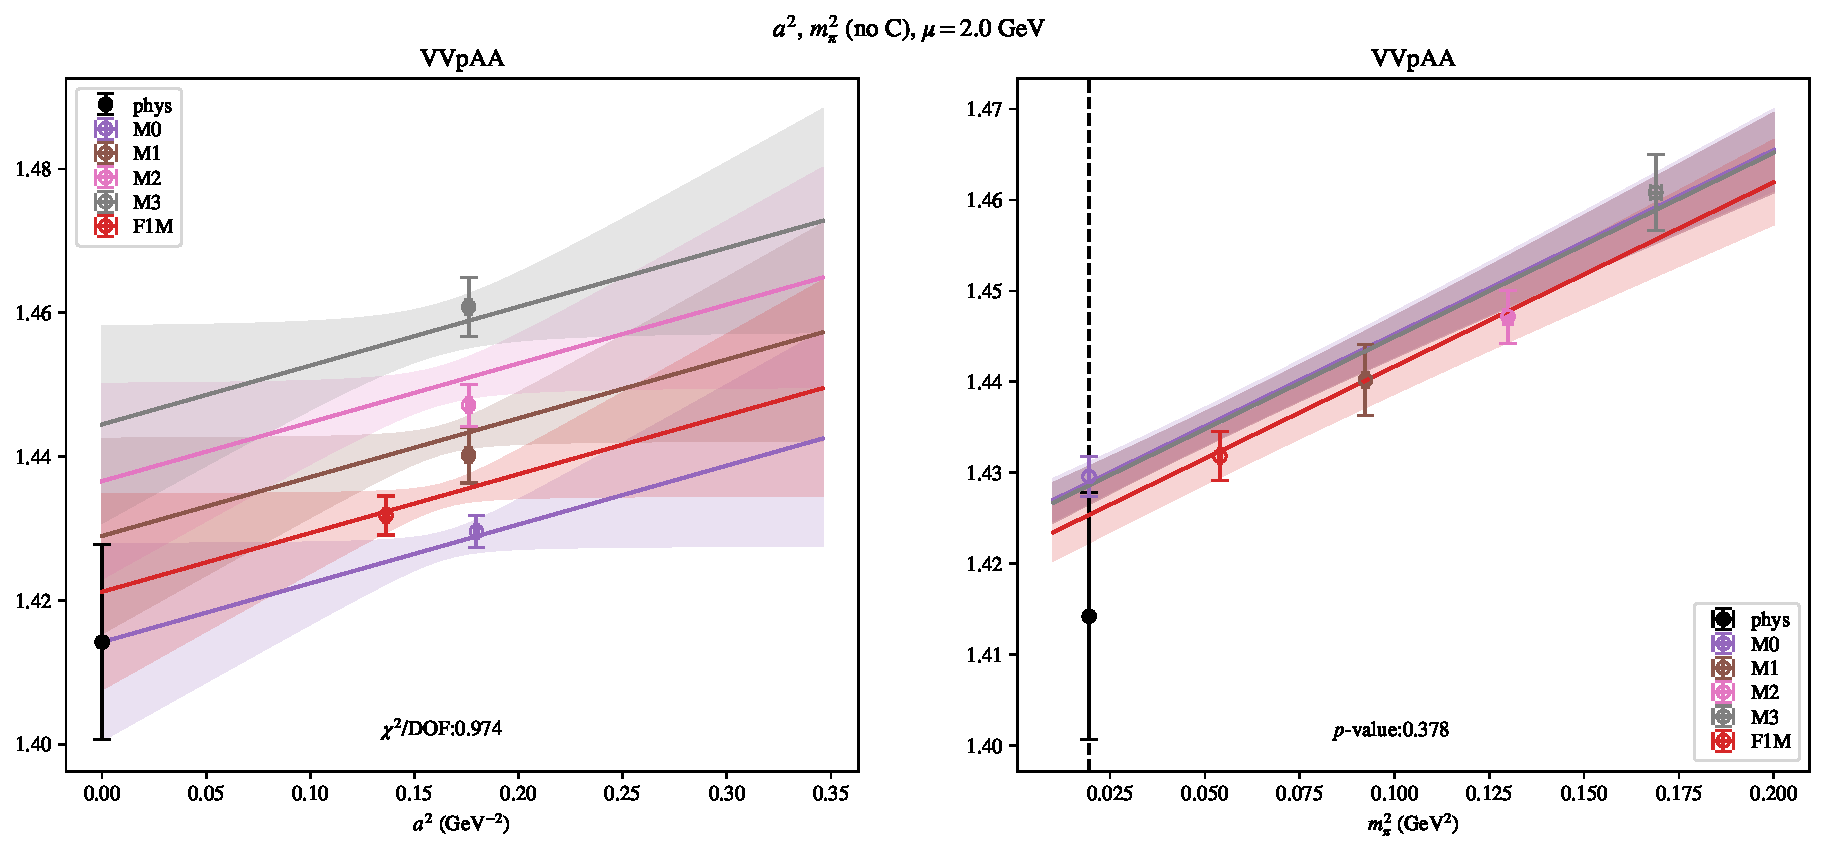
\includepdf[link, pages=-]{VVpAA/NPR/a2m2noC_20.pdf}
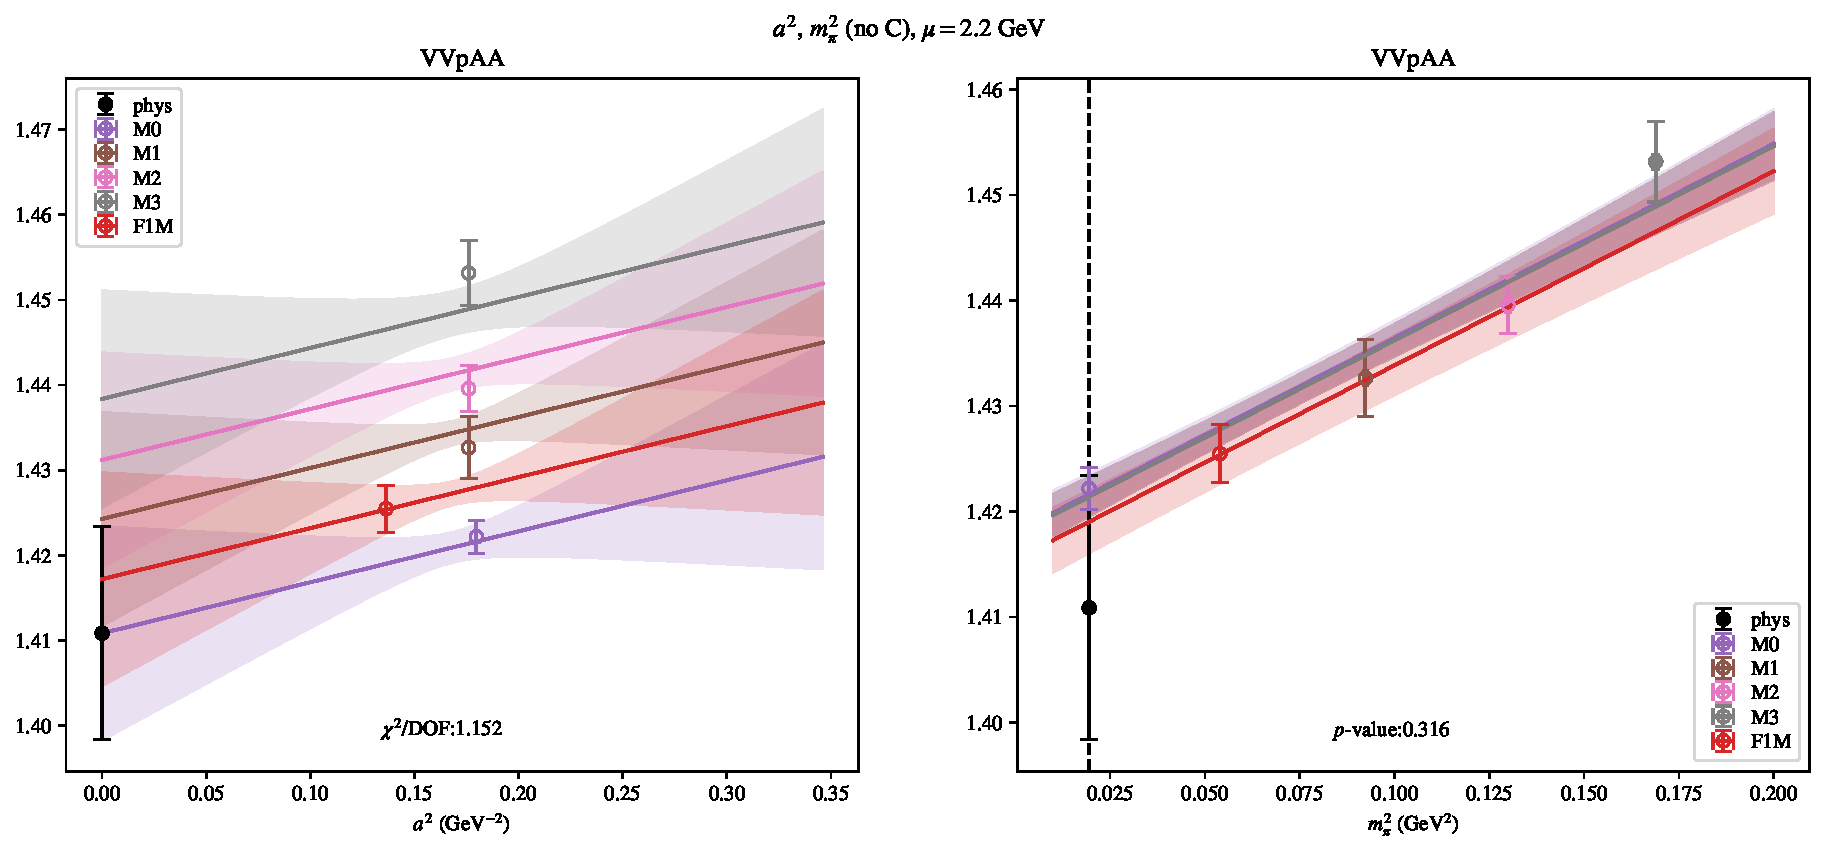
\includepdf[link, pages=-]{VVpAA/NPR/a2m2noC_22.pdf}
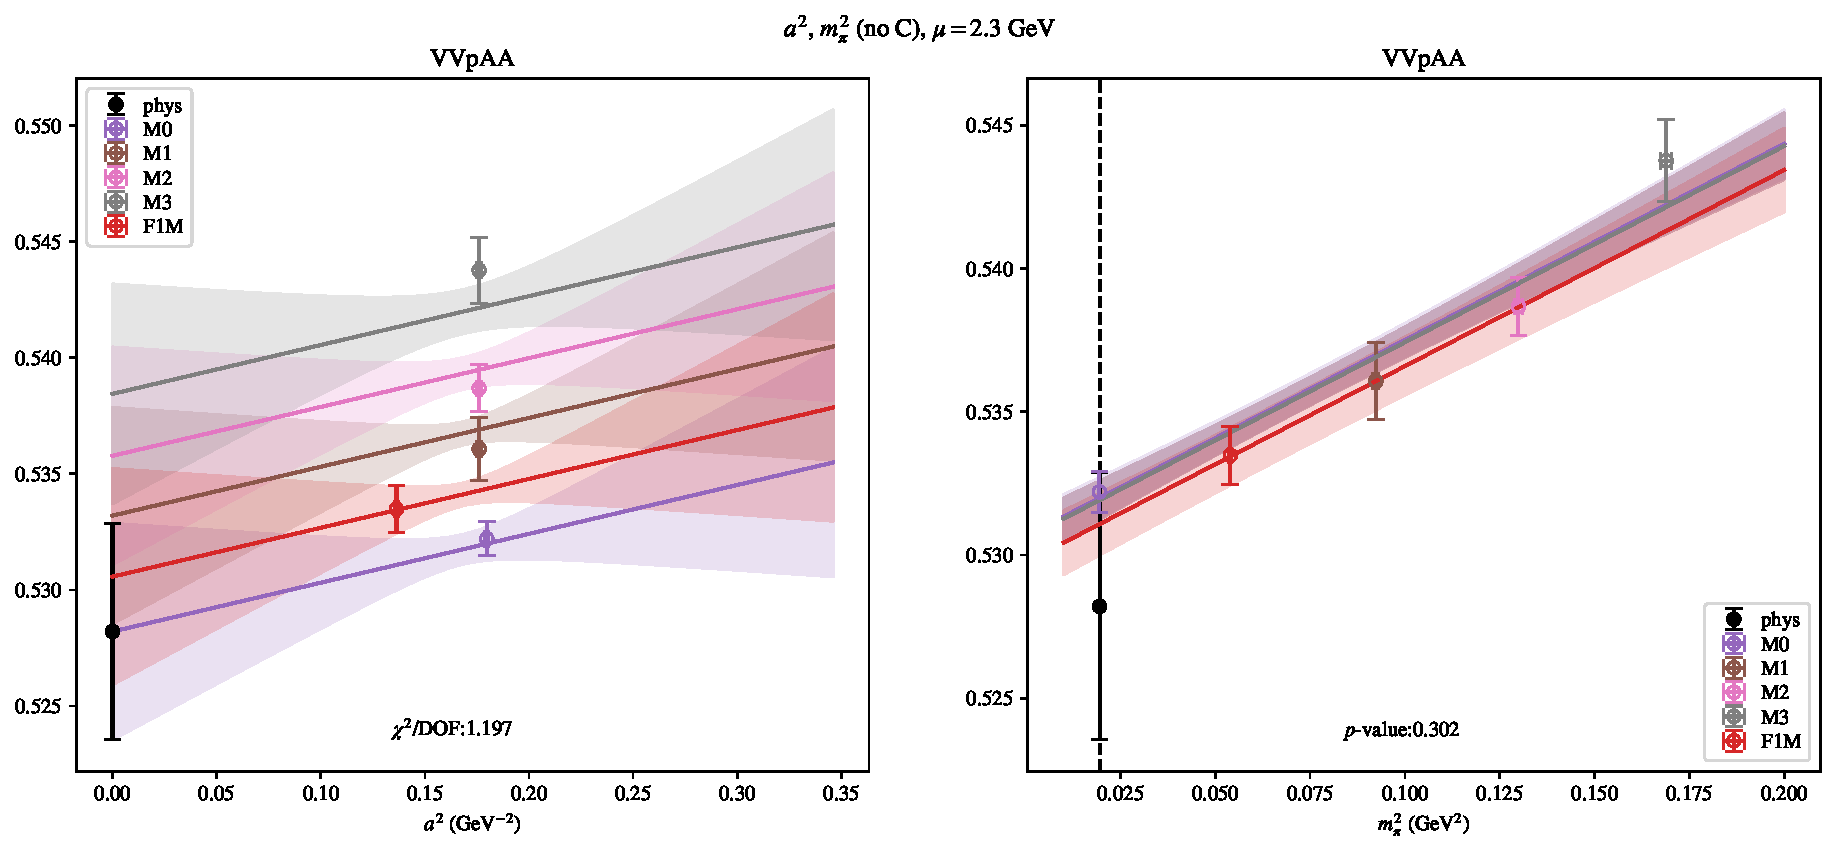
\includepdf[link, pages=-]{VVpAA/NPR/a2m2noC_23.pdf}
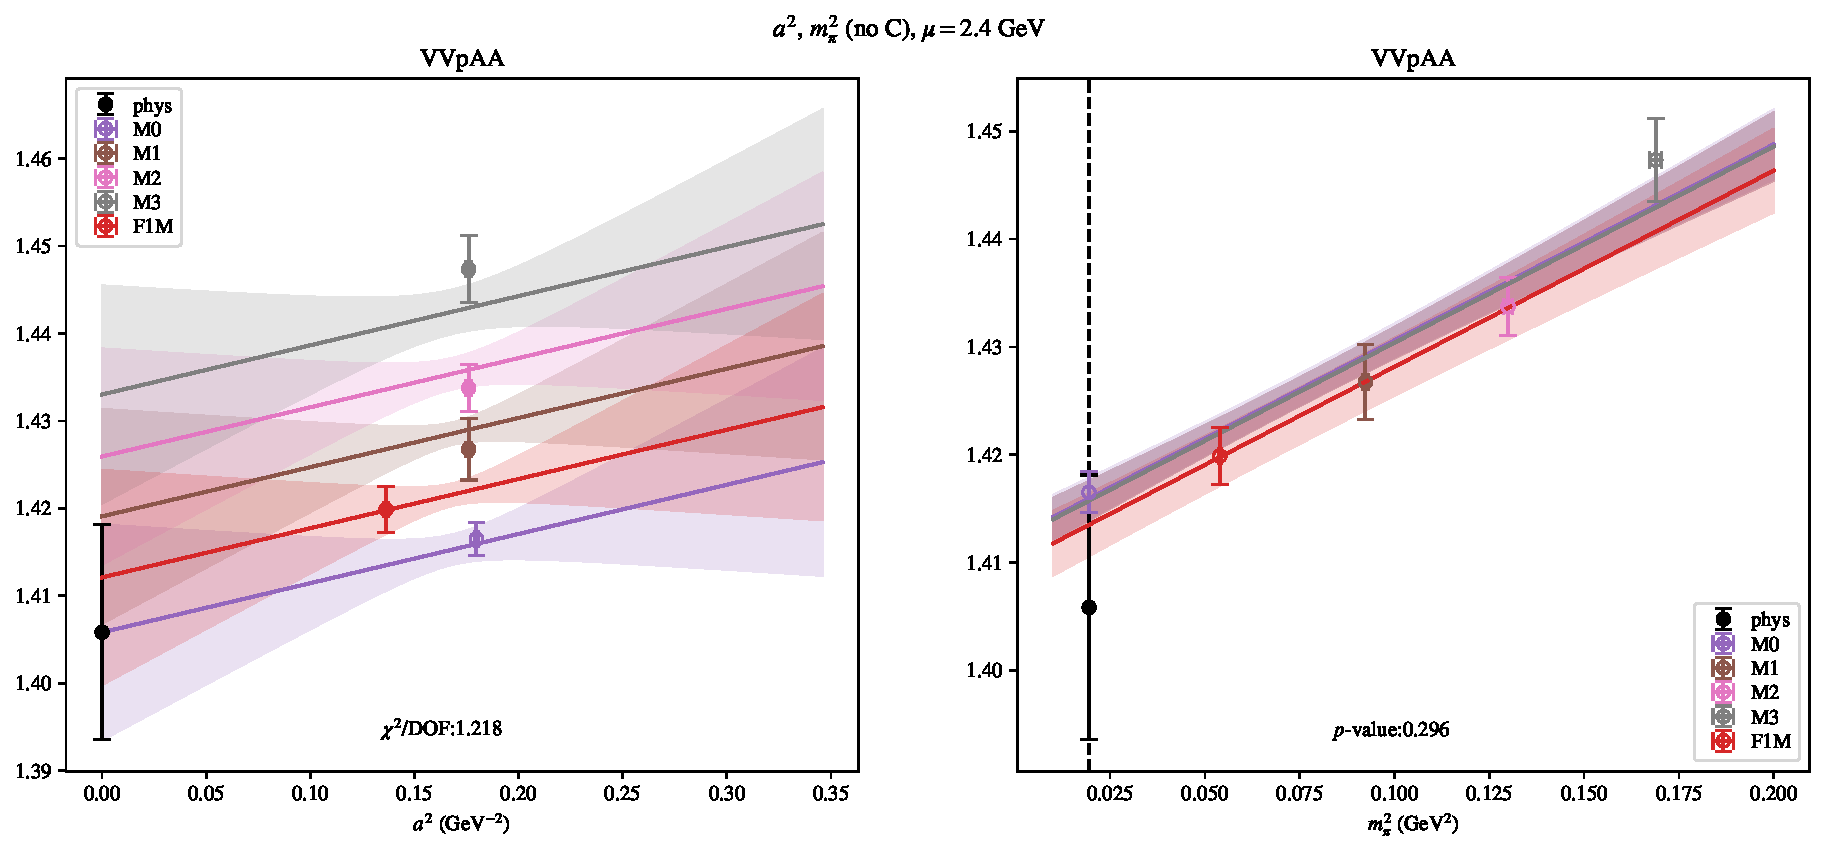
\includepdf[link, pages=-]{VVpAA/NPR/a2m2noC_24.pdf}
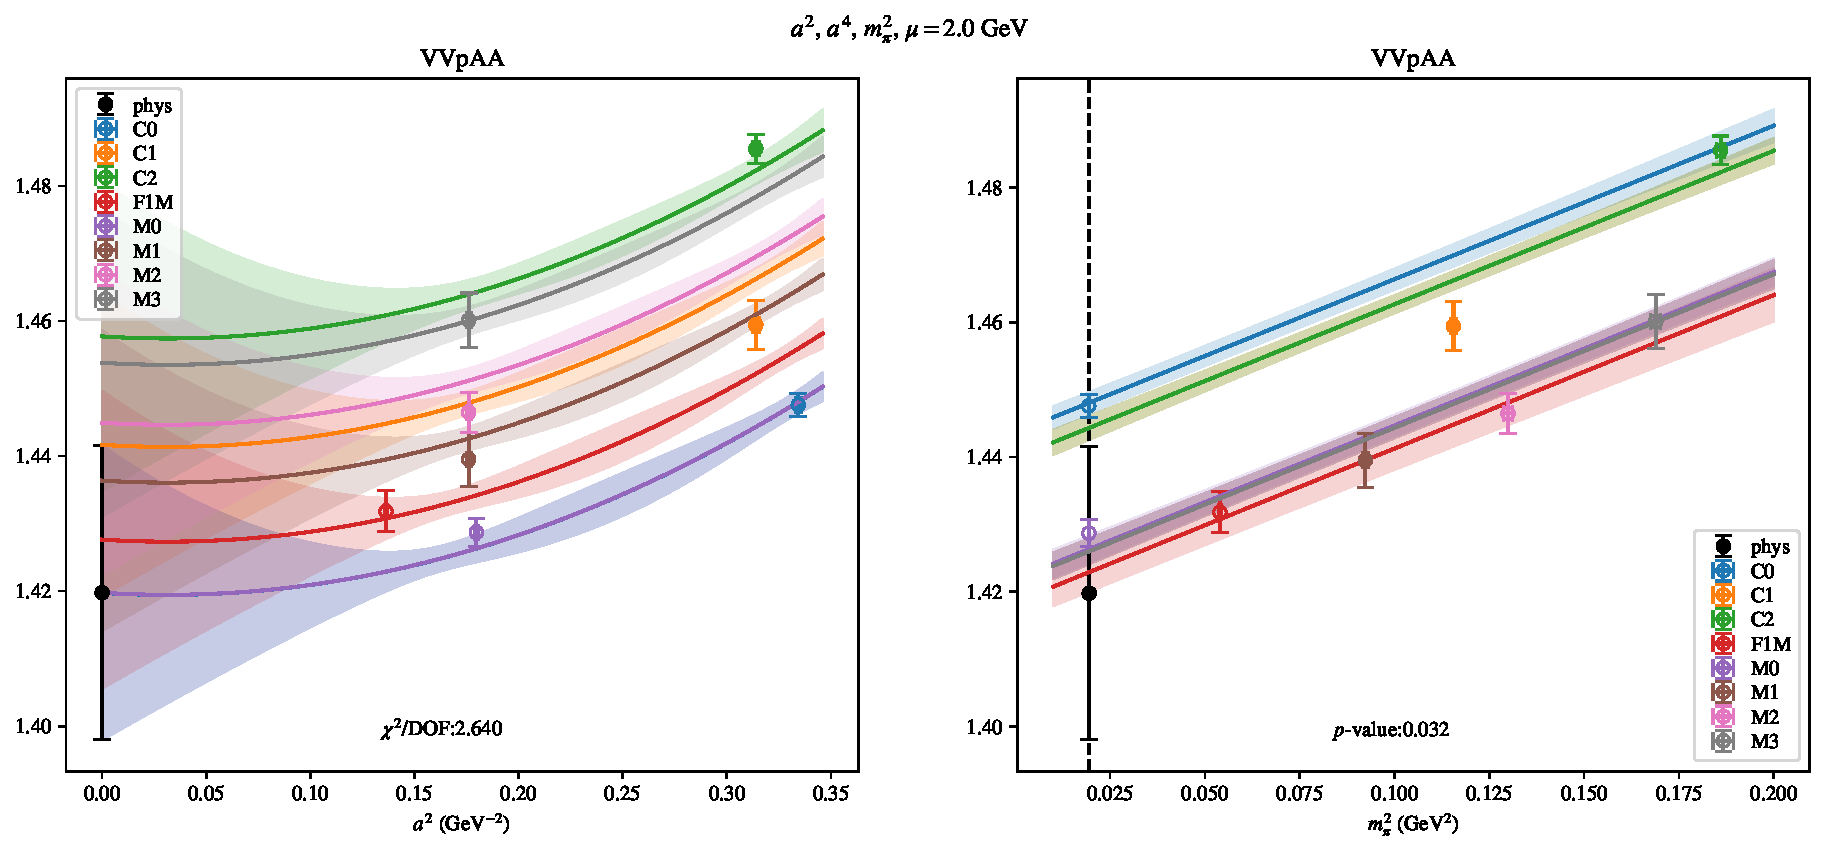
\includepdf[link, pages=-]{VVpAA/NPR/a2a4m2_20.pdf}
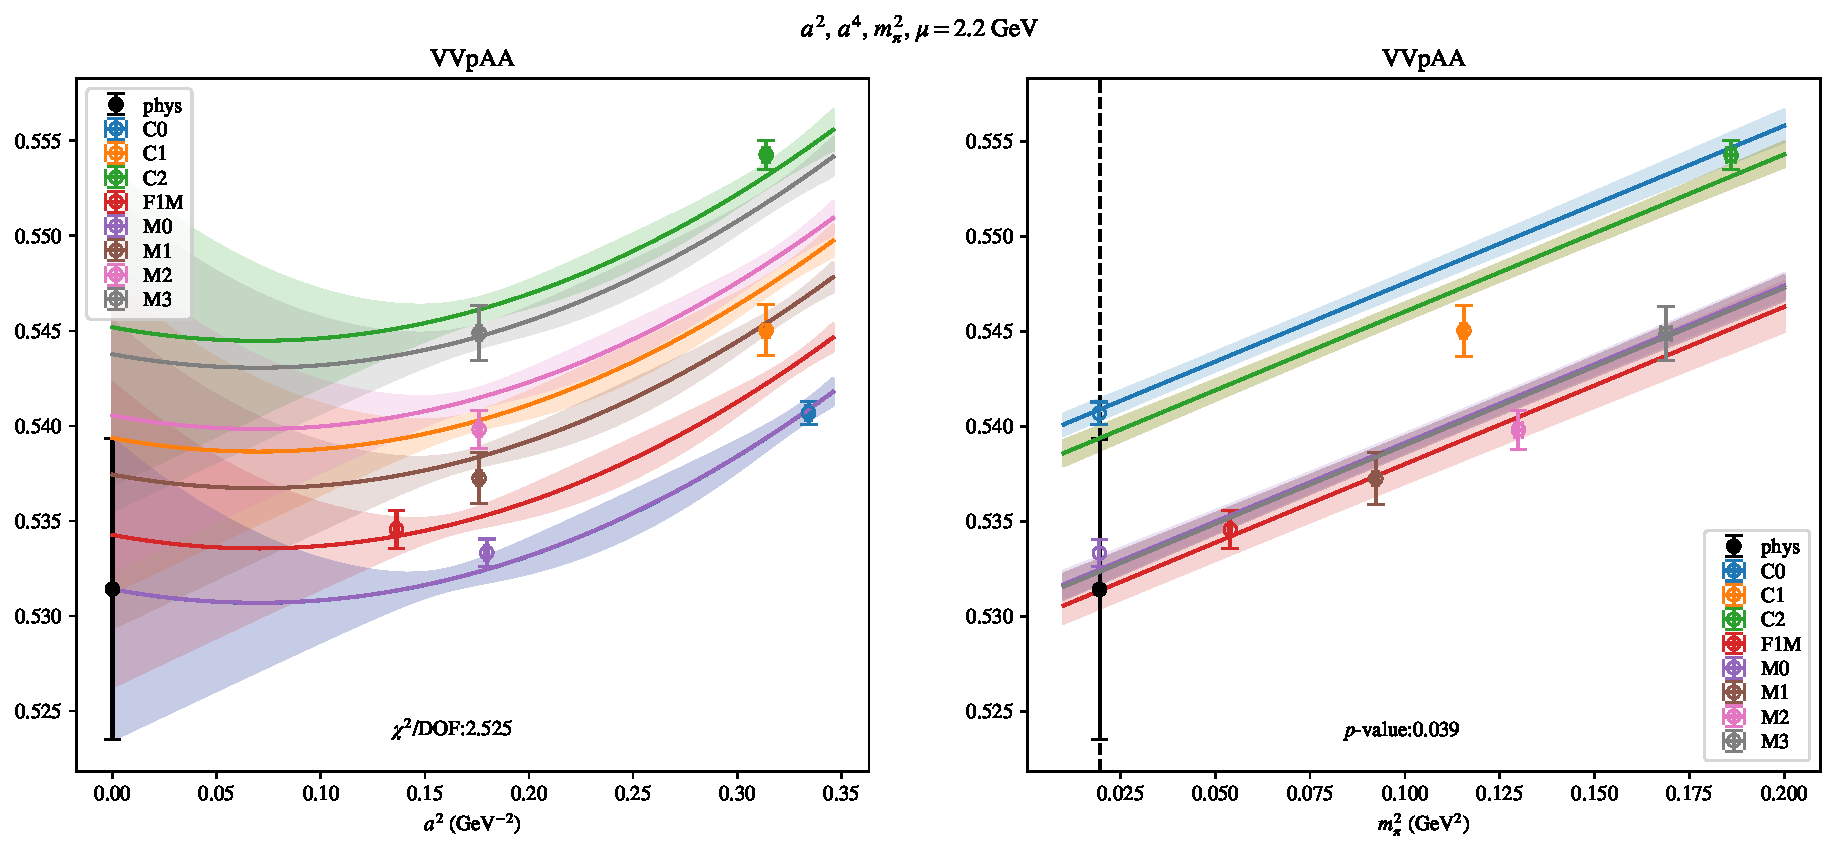
\includepdf[link, pages=-]{VVpAA/NPR/a2a4m2_22.pdf}
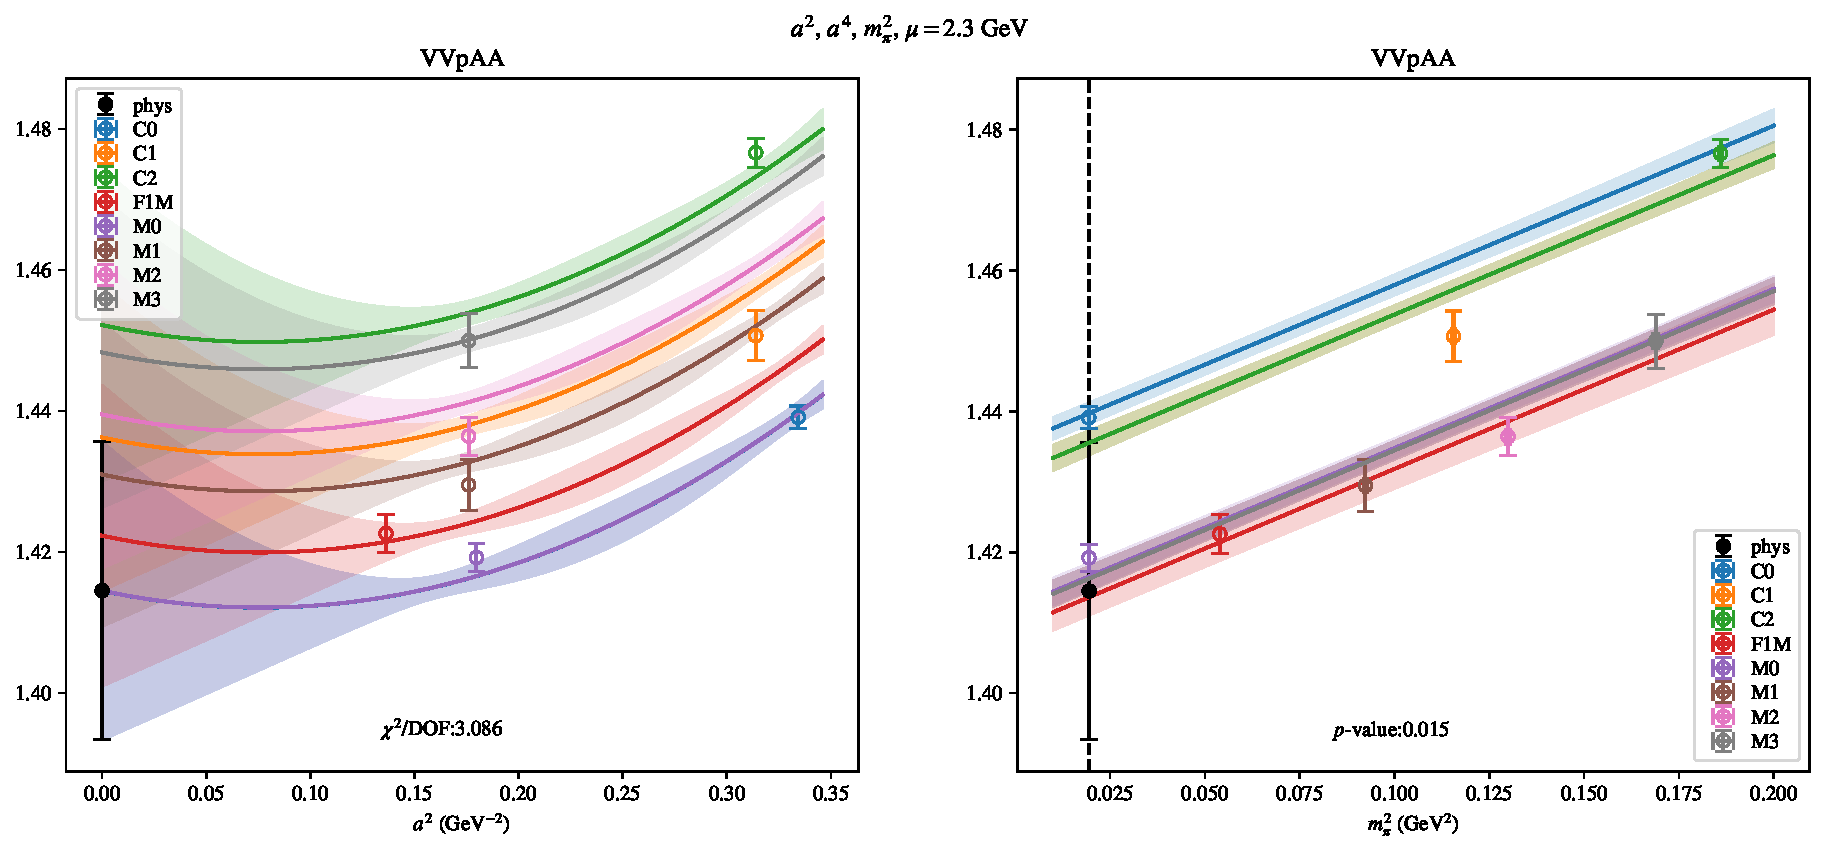
\includepdf[link, pages=-]{VVpAA/NPR/a2a4m2_23.pdf}
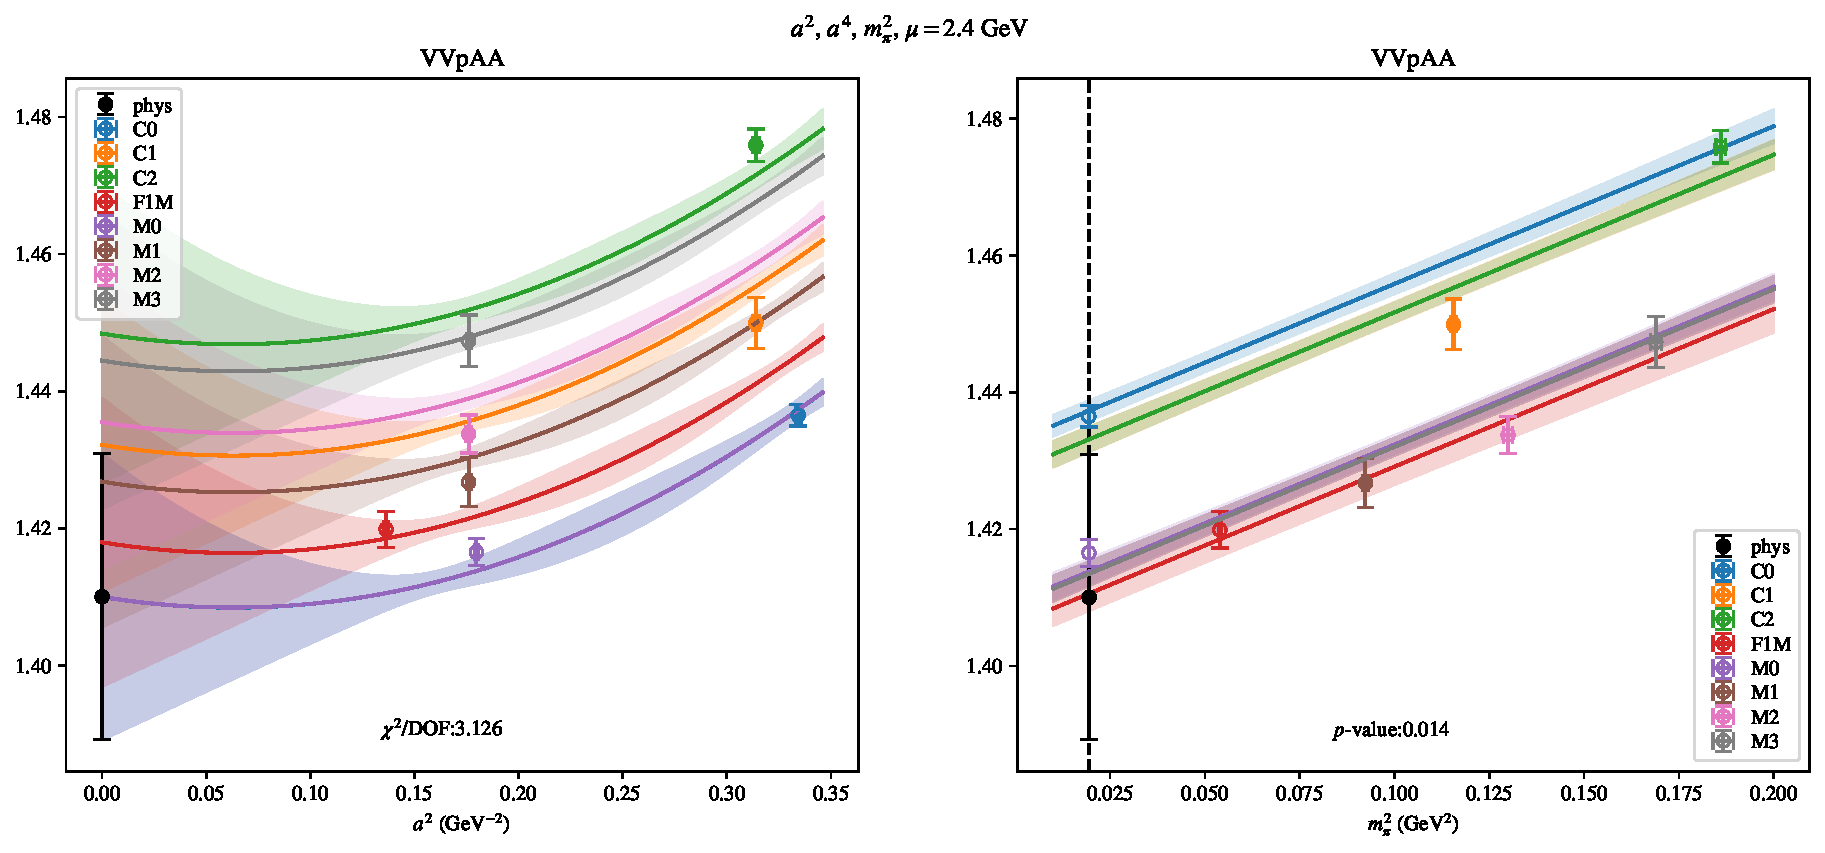
\includepdf[link, pages=-]{VVpAA/NPR/a2a4m2_24.pdf}
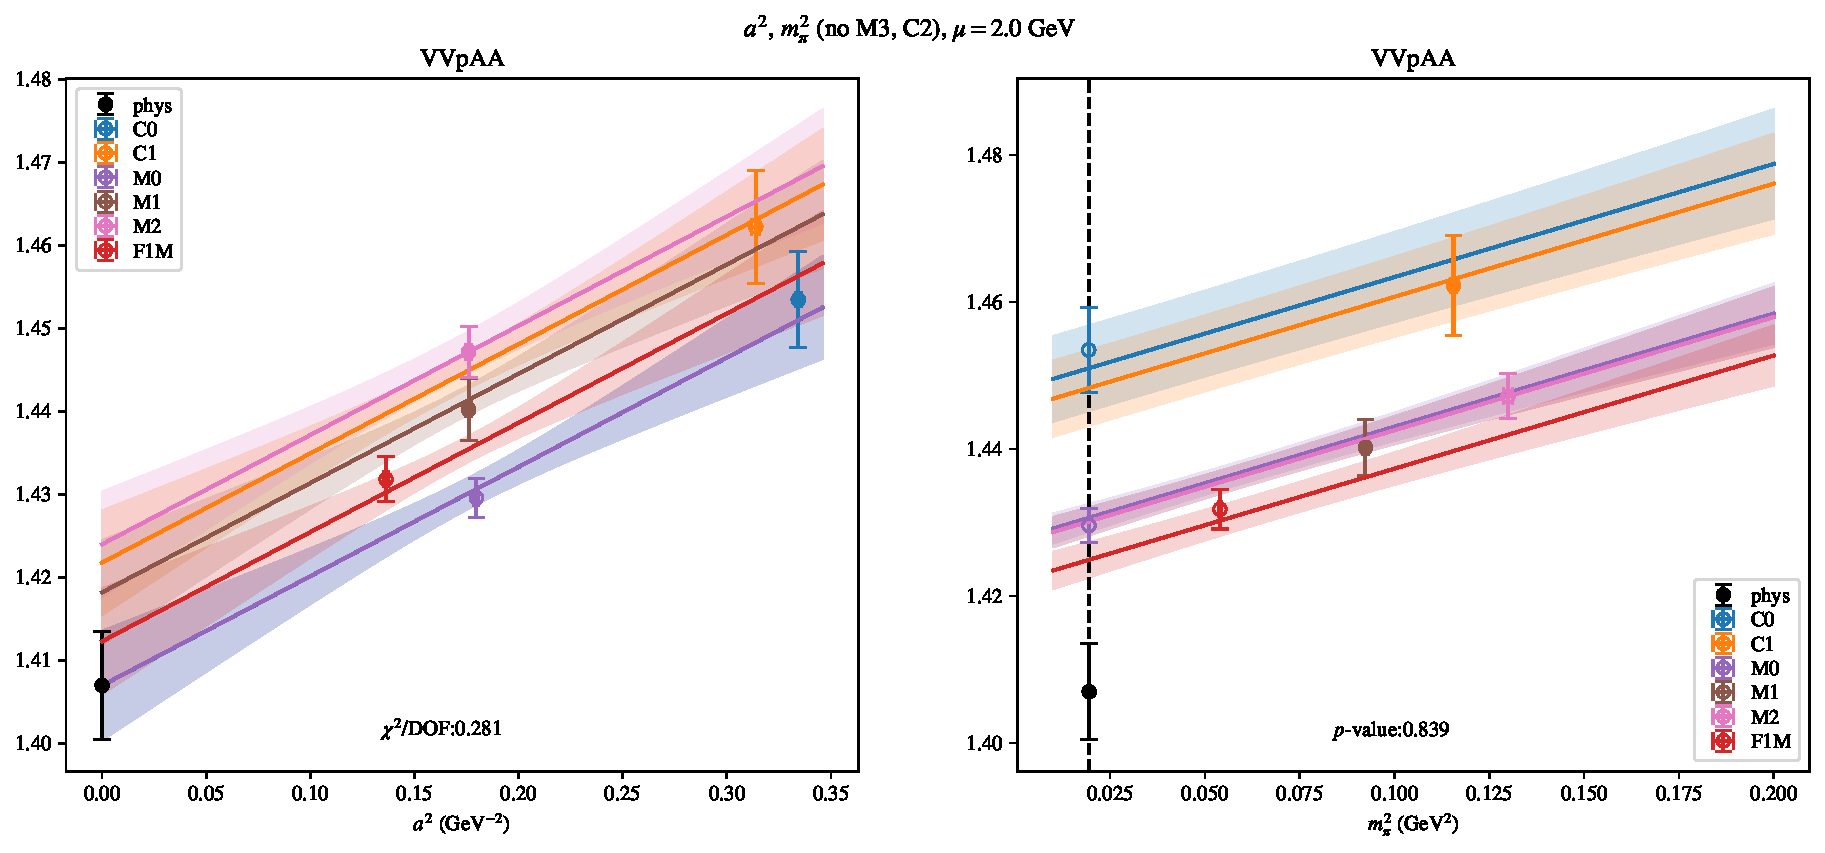
\includepdf[link, pages=-]{VVpAA/NPR/a2m2mcut_20.pdf}
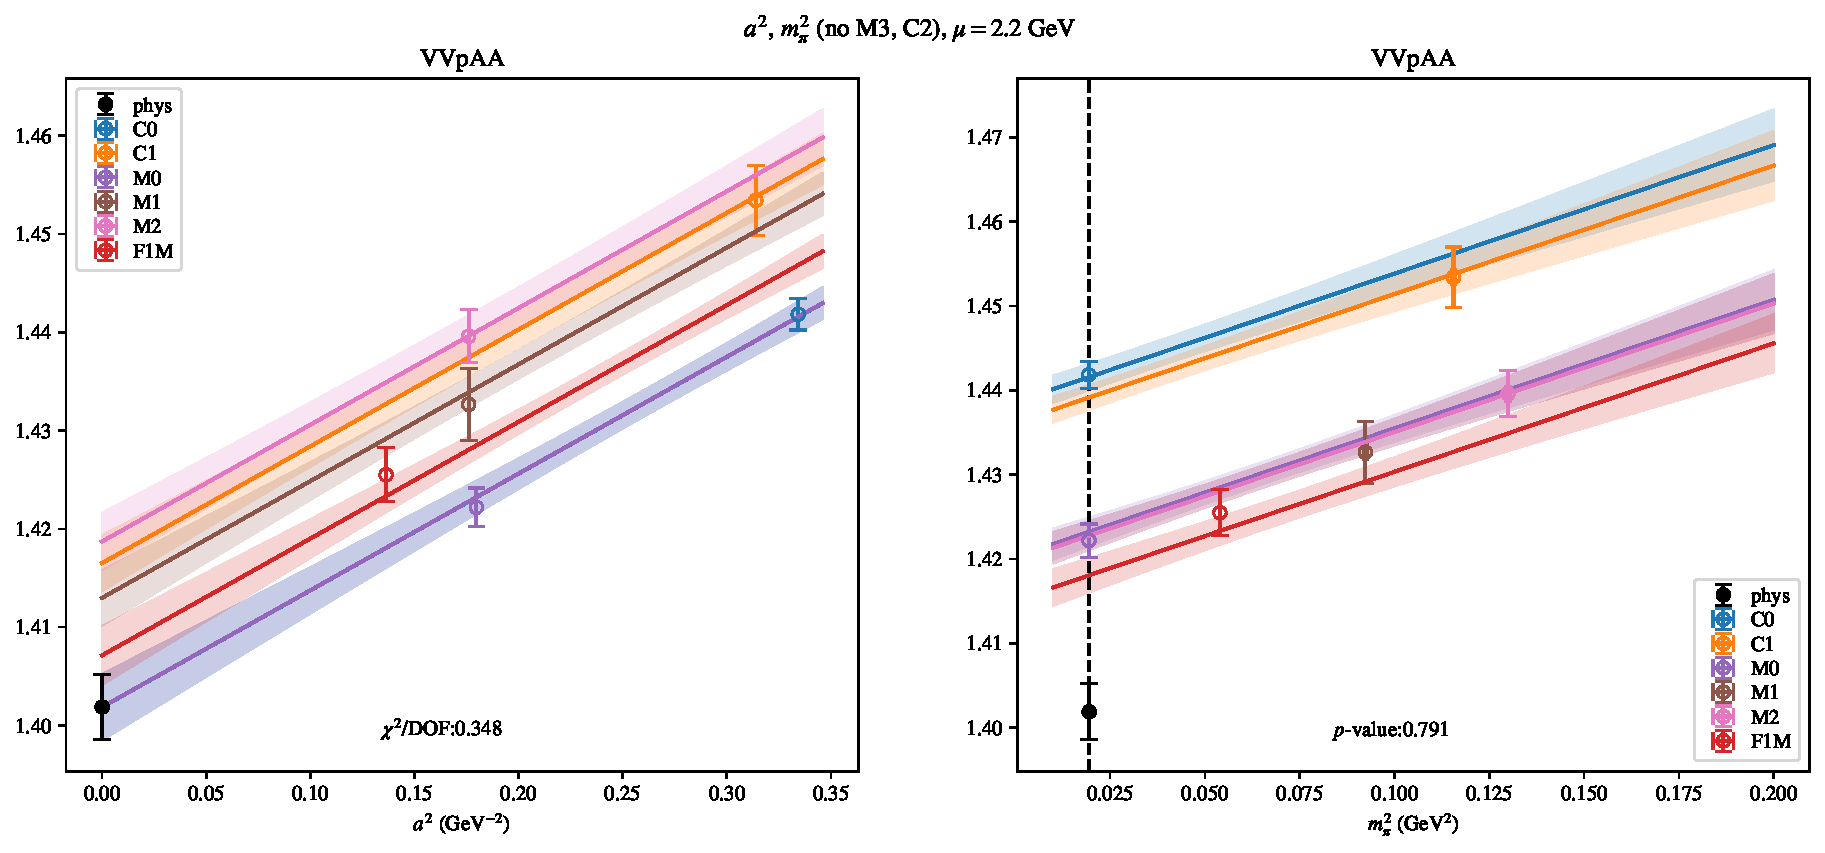
\includepdf[link, pages=-]{VVpAA/NPR/a2m2mcut_22.pdf}
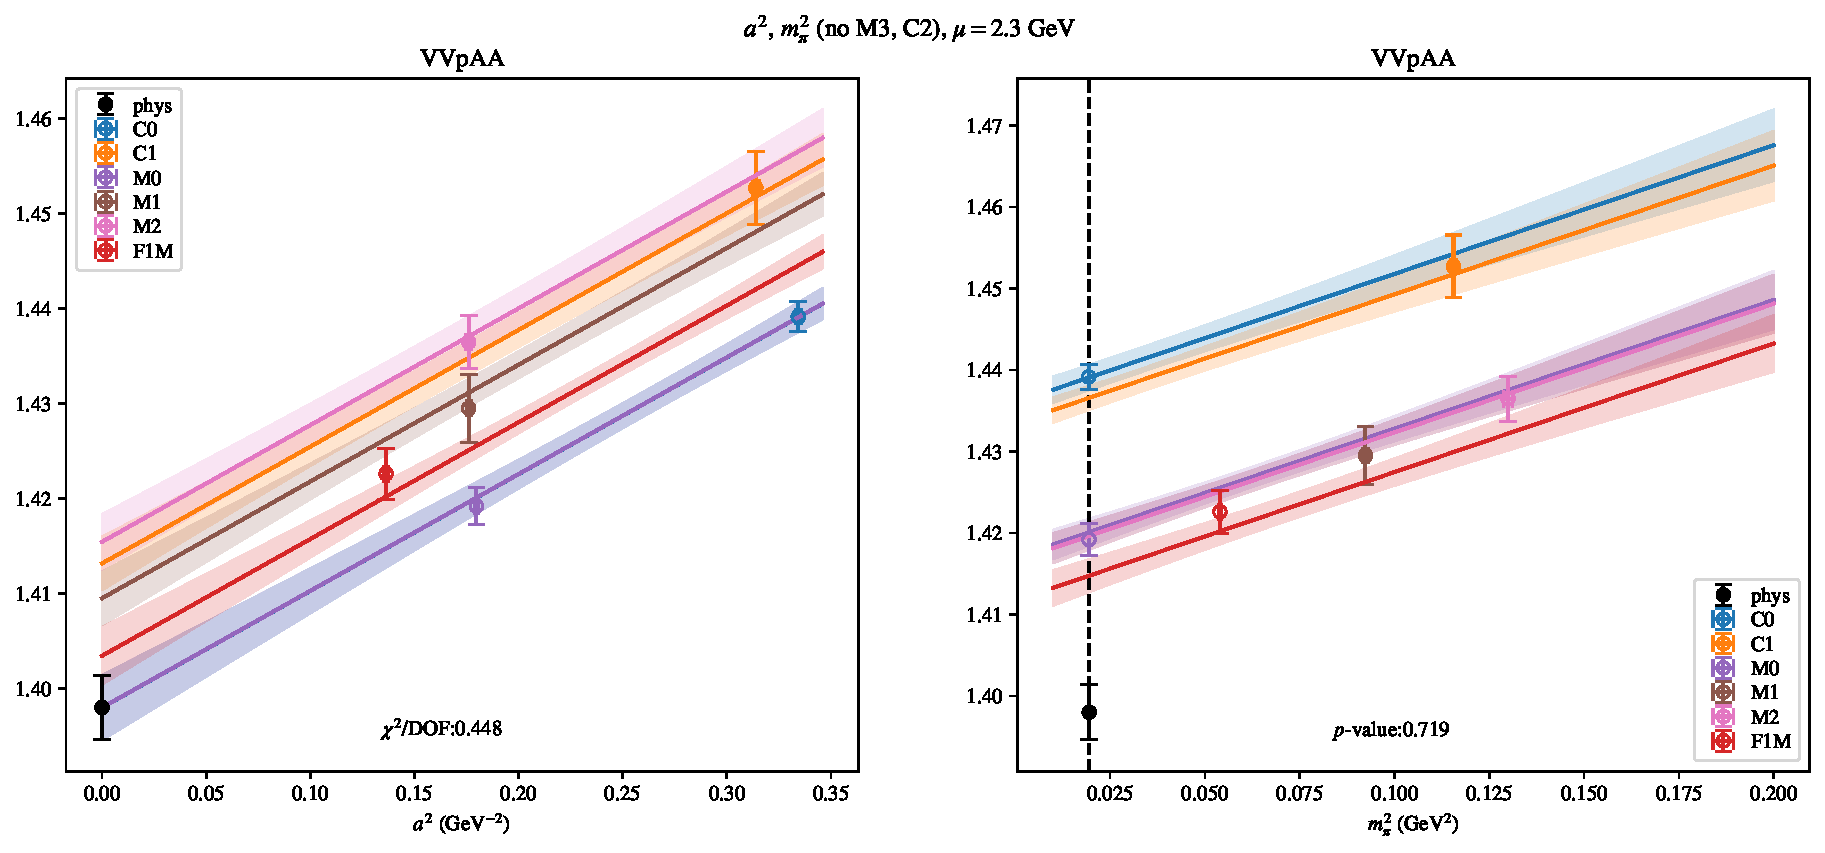
\includepdf[link, pages=-]{VVpAA/NPR/a2m2mcut_23.pdf}
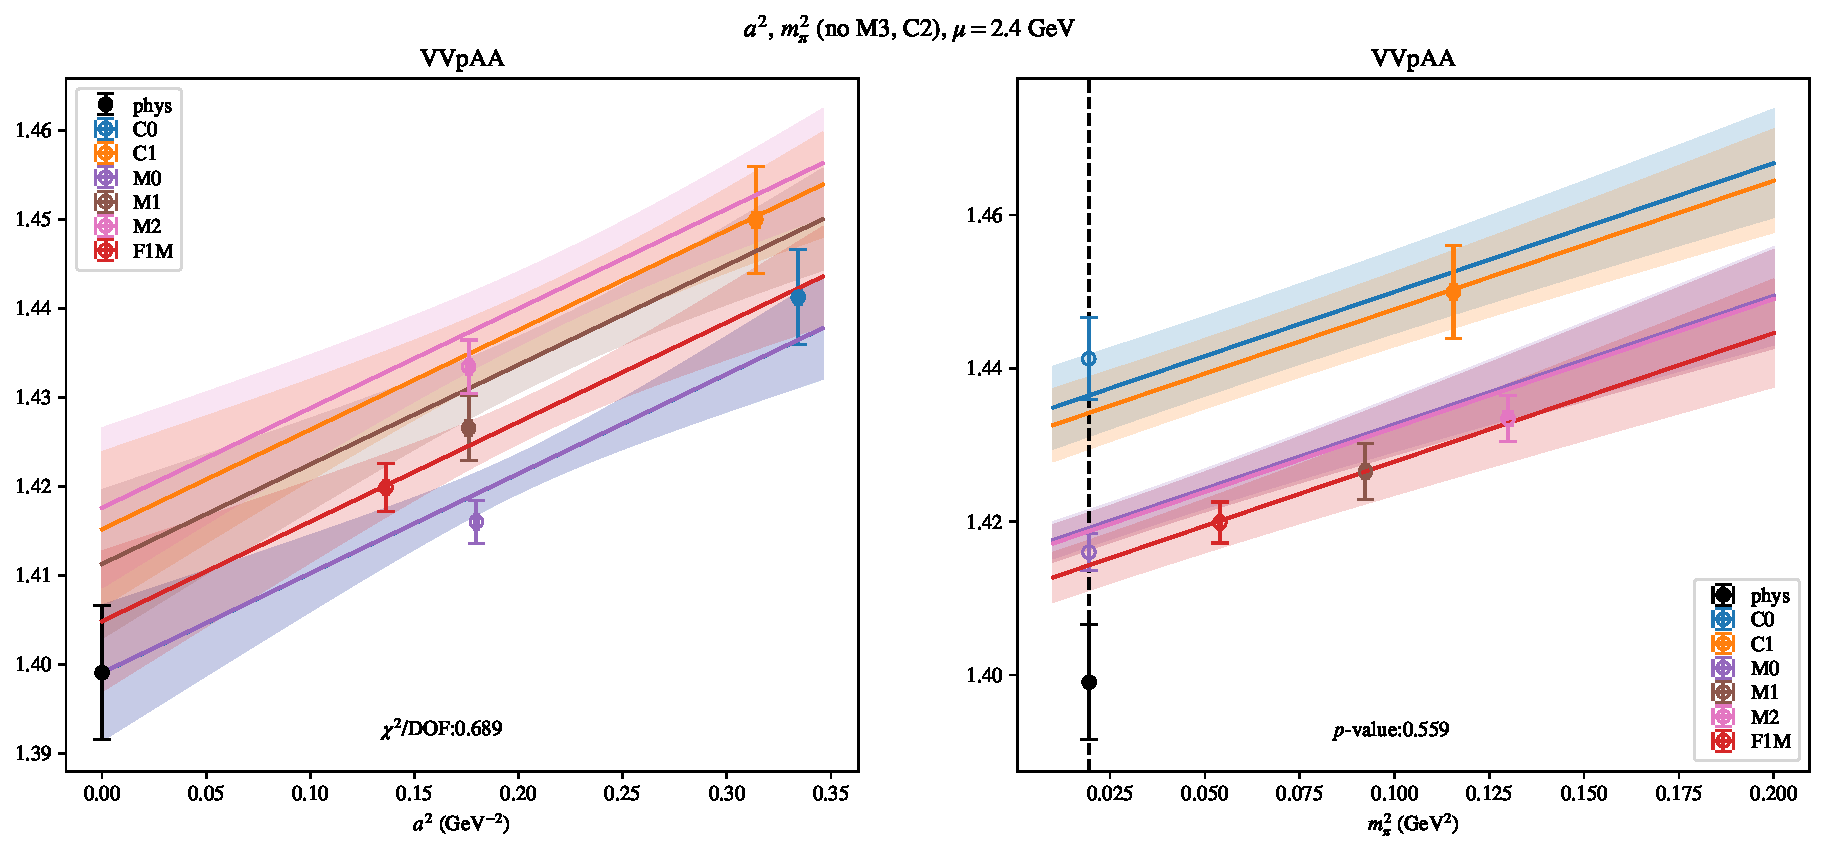
\includepdf[link, pages=-]{VVpAA/NPR/a2m2mcut_24.pdf}
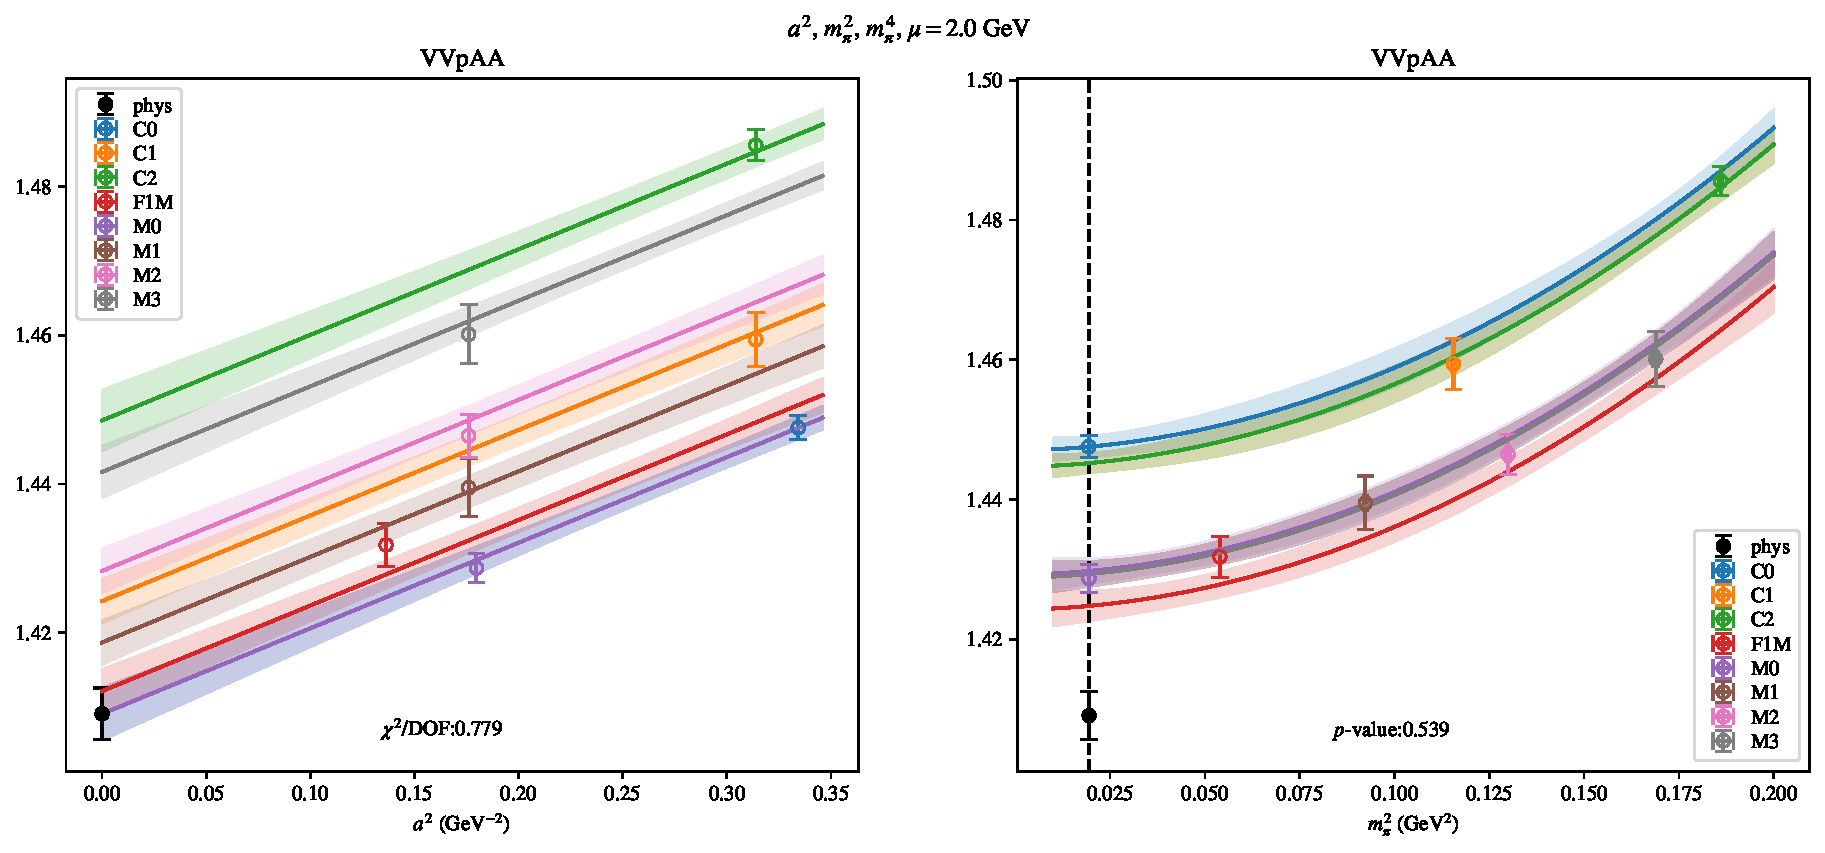
\includepdf[link, pages=-]{VVpAA/NPR/a2m2m4_20.pdf}
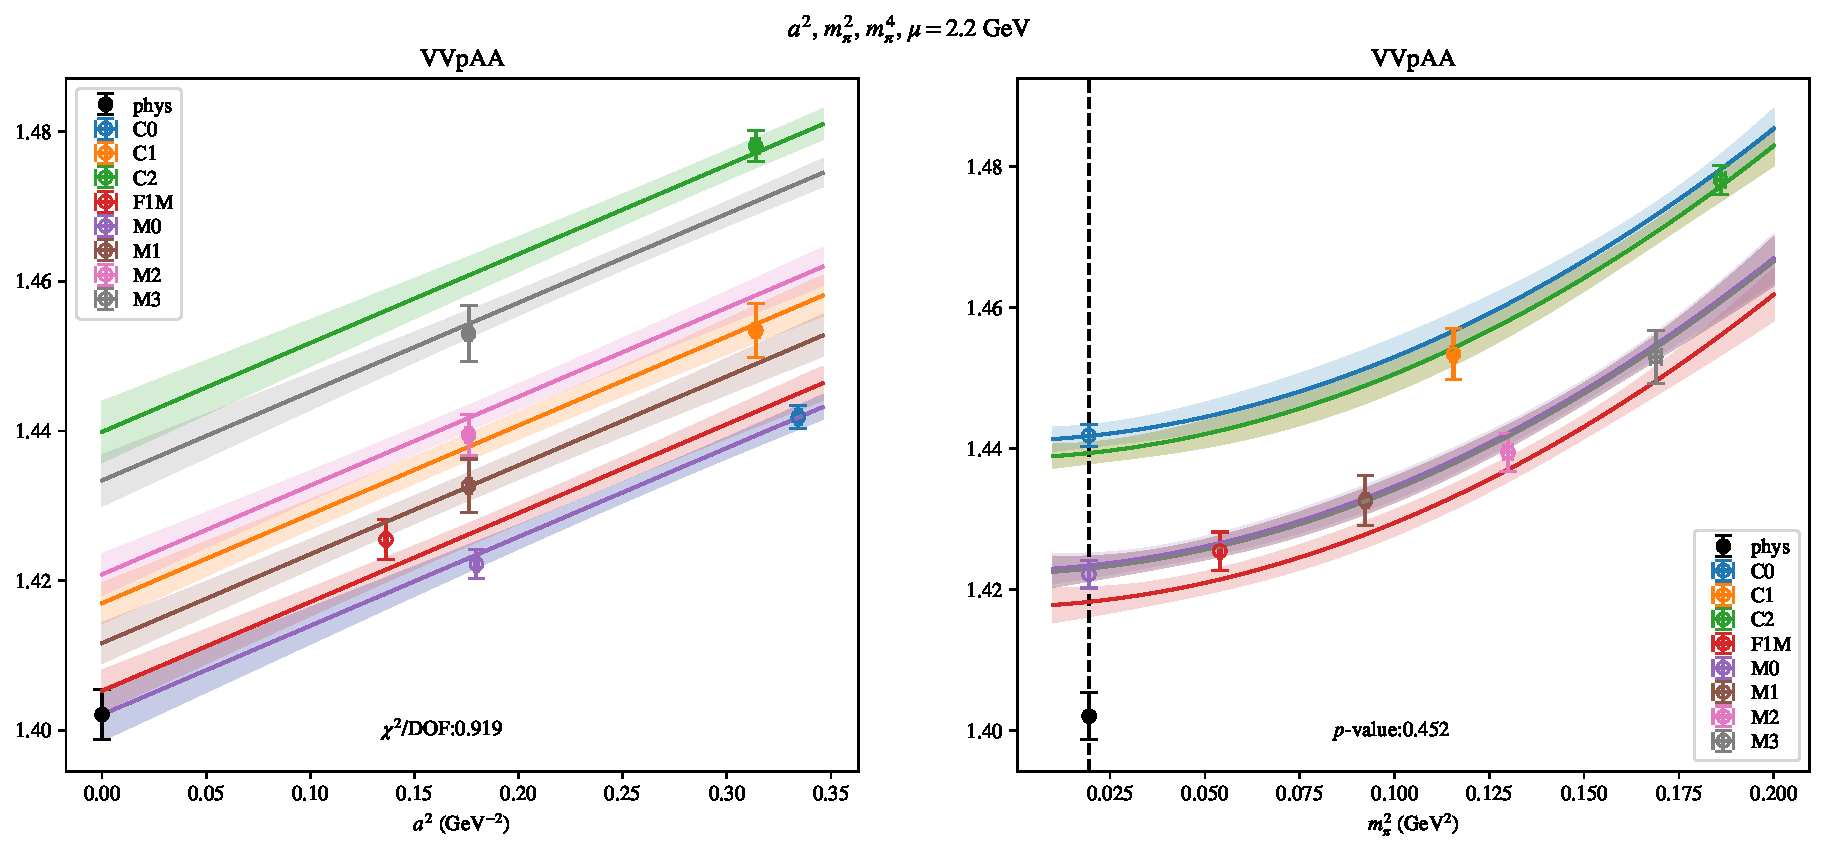
\includepdf[link, pages=-]{VVpAA/NPR/a2m2m4_22.pdf}
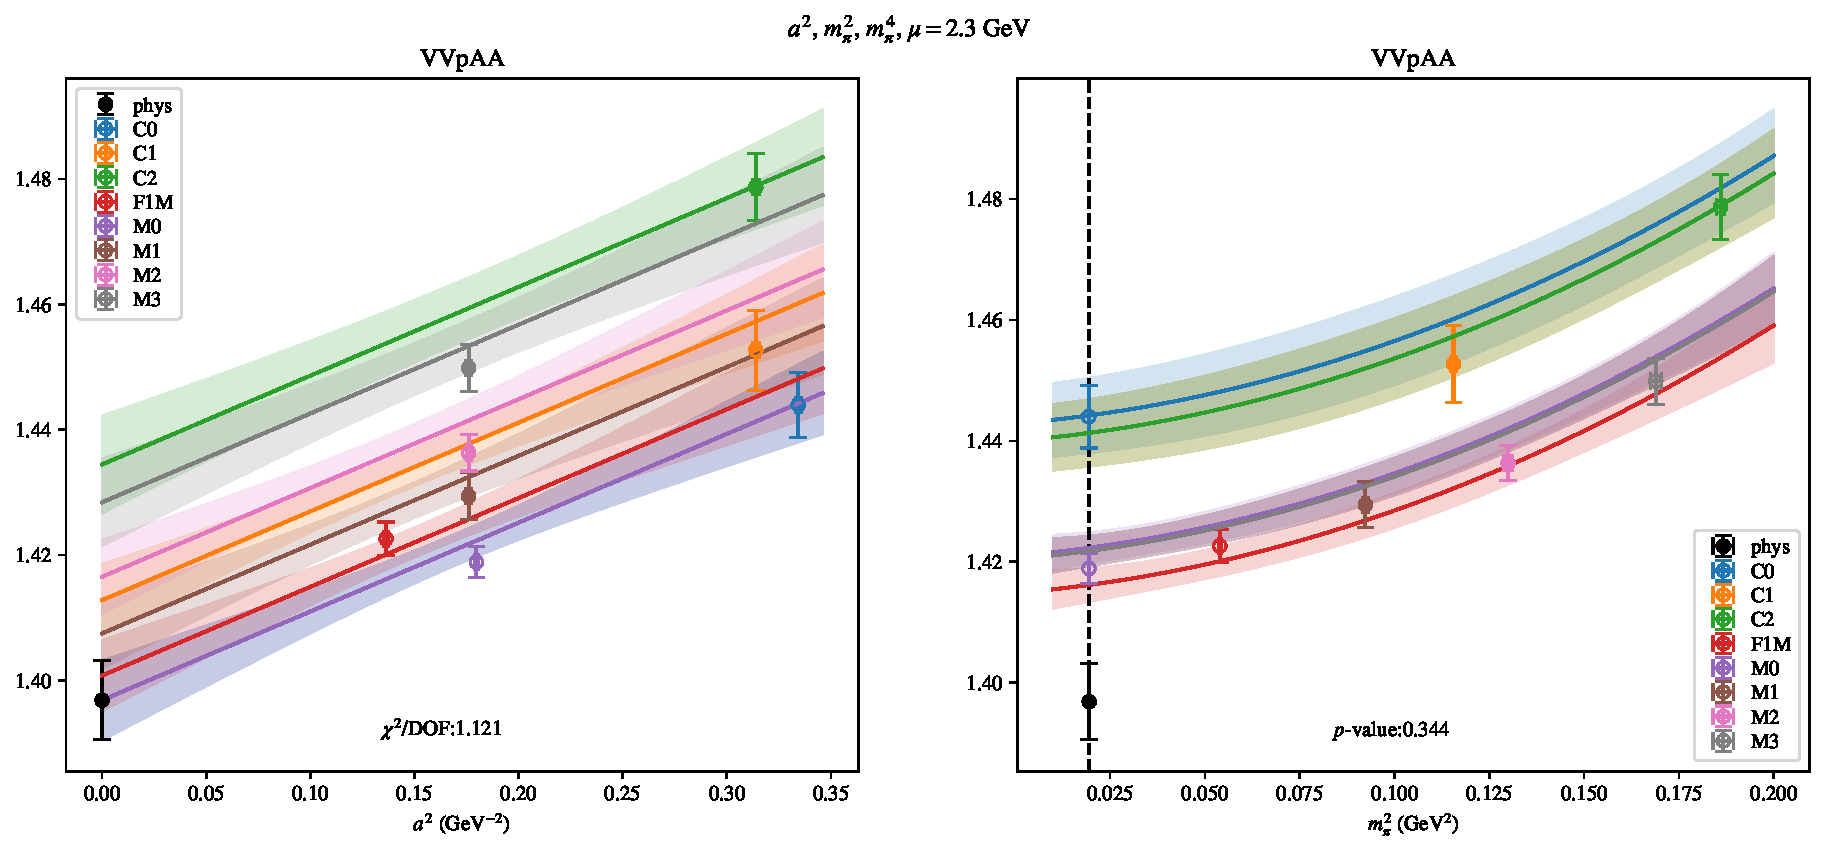
\includepdf[link, pages=-]{VVpAA/NPR/a2m2m4_23.pdf}
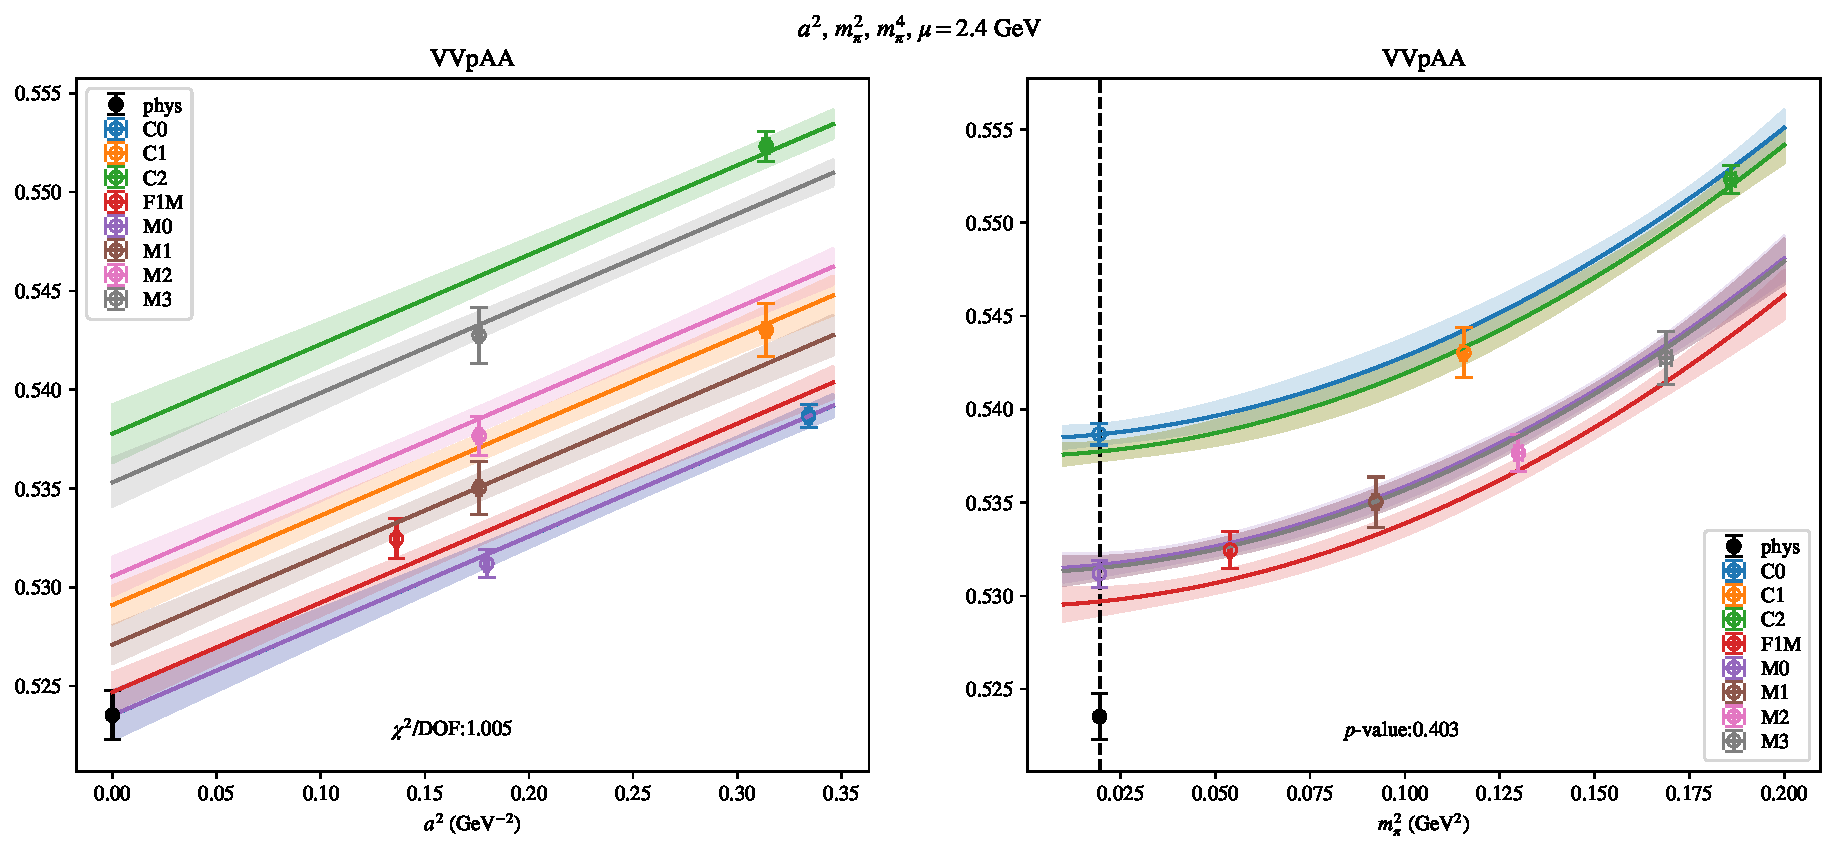
\includepdf[link, pages=-]{VVpAA/NPR/a2m2m4_24.pdf}
\clearpage
\section{$\mathcal{B}_2$}
\begin{table}[h!]
\begin{center}
\begin{tabular}{|c|c|c|c|c|c|}
\hline
$\mu$ (GeV) & $a^2$, $m_\pi^2$& $a^2$, $m_\pi^2$ (no C)& $a^2$, $a^4$, $m_\pi^2$& $a^2$, $m_\pi^2$ (no M3, C2)& $a^2$, $m_\pi^2$, $m_\pi^4$\\
\hline
2.0& \hyperlink{VVmAA/NPR/a2m2_20.pdf.1}{\textbf{-1(13)}: 30383.989 (0.0)} & \hyperlink{VVmAA/NPR/a2m2noC_20.pdf.1}{\textbf{29(63)}: 40323.739 (0.0)} & \hyperlink{VVmAA/NPR/a2a4m2_20.pdf.1}{\textbf{-(12)}: 36955.597 (0.0)} & \hyperlink{VVmAA/NPR/a2m2mcut_20.pdf.1}{\textbf{-2(30)}: 23066.07 (0.0)} & \hyperlink{VVmAA/NPR/a2m2m4_20.pdf.1}{\textbf{-2(16)}: 6265.725 (0.0)}\\
2.2& \hyperlink{VVmAA/NPR/a2m2_22.pdf.1}{\textbf{-1(13)}: 30579.93 (0.0)} & \hyperlink{VVmAA/NPR/a2m2noC_22.pdf.1}{\textbf{27(61)}: 40704.4 (0.0)} & \hyperlink{VVmAA/NPR/a2a4m2_22.pdf.1}{\textbf{-(12)}: 37303.488 (0.0)} & \hyperlink{VVmAA/NPR/a2m2mcut_22.pdf.1}{\textbf{-2(30)}: 23217.938 (0.0)} & \hyperlink{VVmAA/NPR/a2m2m4_22.pdf.1}{\textbf{-2(15)}: 6322.07 (0.0)}\\
2.3& \hyperlink{VVmAA/NPR/a2m2_23.pdf.1}{\textbf{-1(13)}: 30627.412 (0.0)} & \hyperlink{VVmAA/NPR/a2m2noC_23.pdf.1}{\textbf{26(60)}: 40815.806 (0.0)} & \hyperlink{VVmAA/NPR/a2a4m2_23.pdf.1}{\textbf{-(12)}: 37408.36 (0.0)} & \hyperlink{VVmAA/NPR/a2m2mcut_23.pdf.1}{\textbf{-2(30)}: 23215.153 (0.0)} & \hyperlink{VVmAA/NPR/a2m2m4_23.pdf.1}{\textbf{-2(15)}: 6328.523 (0.0)}\\
2.4& \hyperlink{VVmAA/NPR/a2m2_24.pdf.1}{\textbf{-1(13)}: 30664.362 (0.0)} & \hyperlink{VVmAA/NPR/a2m2noC_24.pdf.1}{\textbf{26(59)}: 40910.266 (0.0)} & \hyperlink{VVmAA/NPR/a2a4m2_24.pdf.1}{\textbf{-(12)}: 37493.353 (0.0)} & \hyperlink{VVmAA/NPR/a2m2mcut_24.pdf.1}{\textbf{-2(29)}: 23208.695 (0.0)} & \hyperlink{VVmAA/NPR/a2m2m4_24.pdf.1}{\textbf{-2(15)}: 6332.774 (0.0)}\\
\hline
\end{tabular}
\caption{Physical point value from chiral and continuum extrapolation at renormalisation scale $\mu$. Entries are \textbf{value(error)}: $\chi^2/\text{DOF}$ ($p$-value).}
\end{center}
\end{table}
\begin{table}[h!]
\begin{center}
\begin{tabular}{|c c|c|c|c|c|c|}
\hline
$\mu$ (GeV) &  & $a^2$, $m_\pi^2$& $a^2$, $m_\pi^2$ (no C)& $a^2$, $a^4$, $m_\pi^2$& $a^2$, $m_\pi^2$ (no M3, C2)& $a^2$, $m_\pi^2$, $m_\pi^4$\\
\hline
\multirow{2}{0.5in}{2.0} & $\alpha$ & 1.963(57)& -8.78(70)& -7.19(38)& 1.165(64)& 0.416(18)\\
 & $\beta$ & -0.137(15)& 0.0538(14)& -0.0208(55)& -0.181(23)& -0.326(17)\\
\hline
\multirow{2}{0.5in}{2.2} & $\alpha$ & 1.922(56)& -9.00(75)& -7.06(42)& 1.139(64)& 0.401(18)\\
 & $\beta$ & -0.136(15)& 0.0576(15)& -0.0223(61)& -0.180(23)& -0.325(17)\\
\hline
\multirow{2}{0.5in}{2.3} & $\alpha$ & 1.903(56)& -9.10(78)& -7.00(44)& 1.130(63)& 0.395(18)\\
 & $\beta$ & -0.135(15)& 0.0593(15)& -0.0230(63)& -0.180(23)& -0.325(17)\\
\hline
\multirow{2}{0.5in}{2.4} & $\alpha$ & 1.885(55)& -9.19(80)& -6.95(46)& 1.121(63)& 0.389(18)\\
 & $\beta$ & -0.135(15)& 0.0610(16)& -0.0237(66)& -0.180(23)& -0.324(17)\\
\hline
\end{tabular}
\caption{Fit values of coefficients in $Q = Q_{phys} + \mathbf{\alpha} a^2 + \mathbf{\beta}\left(\frac{m_\pi^2}{f_\pi^2}-\frac{m_{\pi,PDG}^2}{f_\pi^2}\right) + \ldots$.}
\end{center}
\end{table}
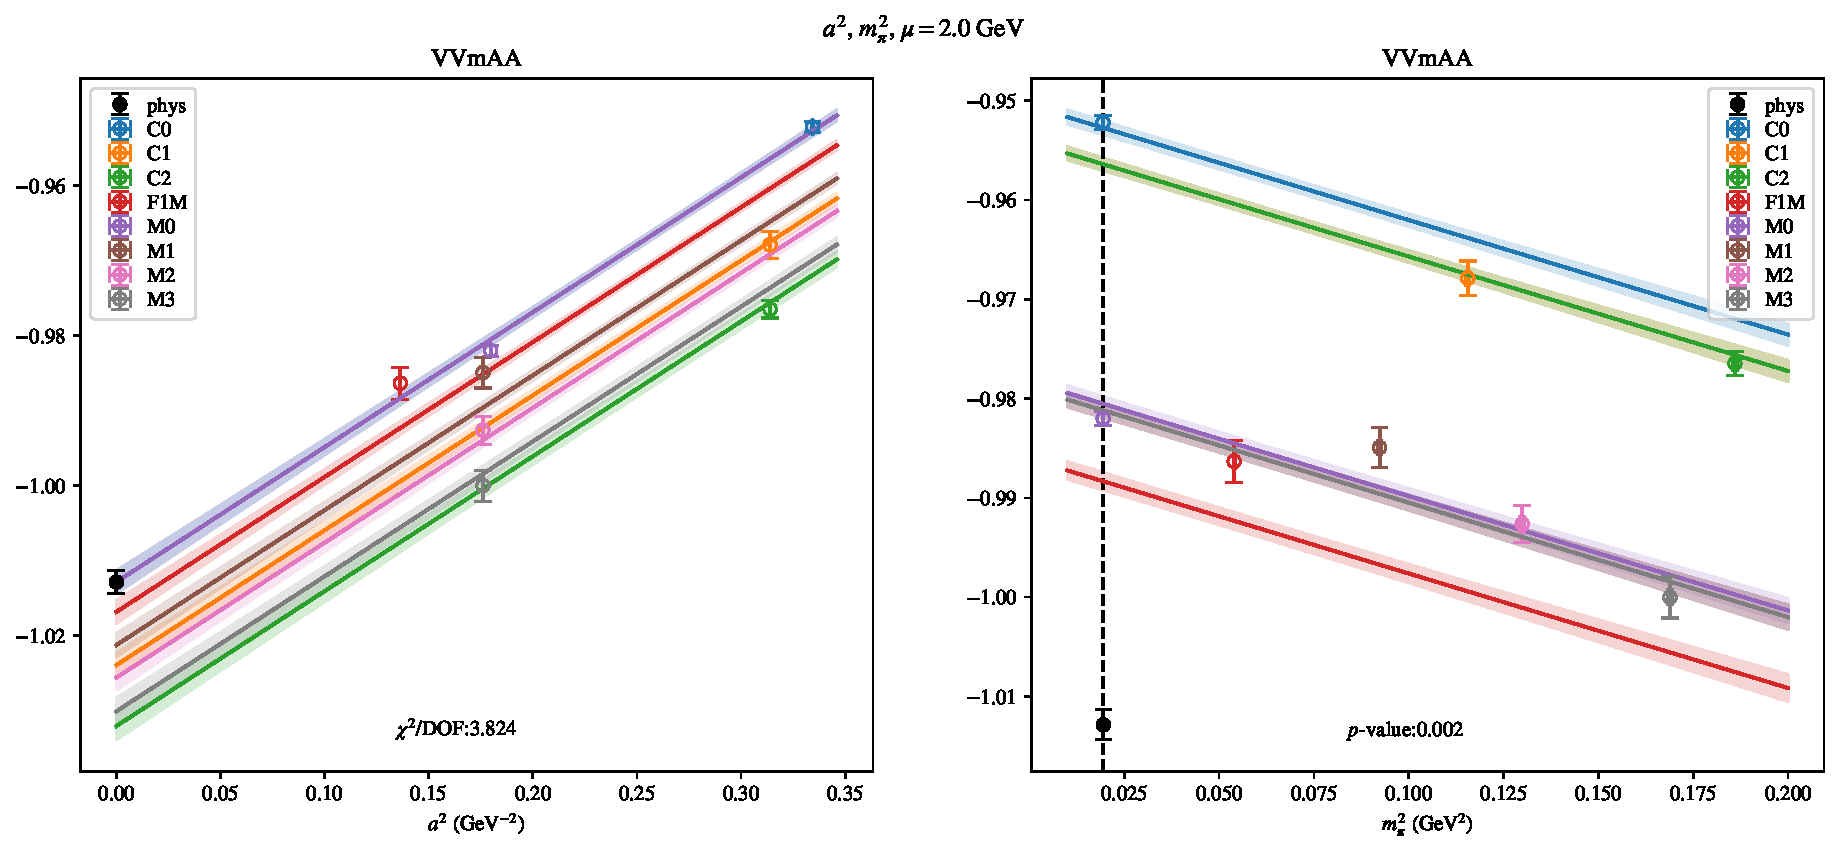
\includepdf[link, pages=-]{VVmAA/NPR/a2m2_20.pdf}
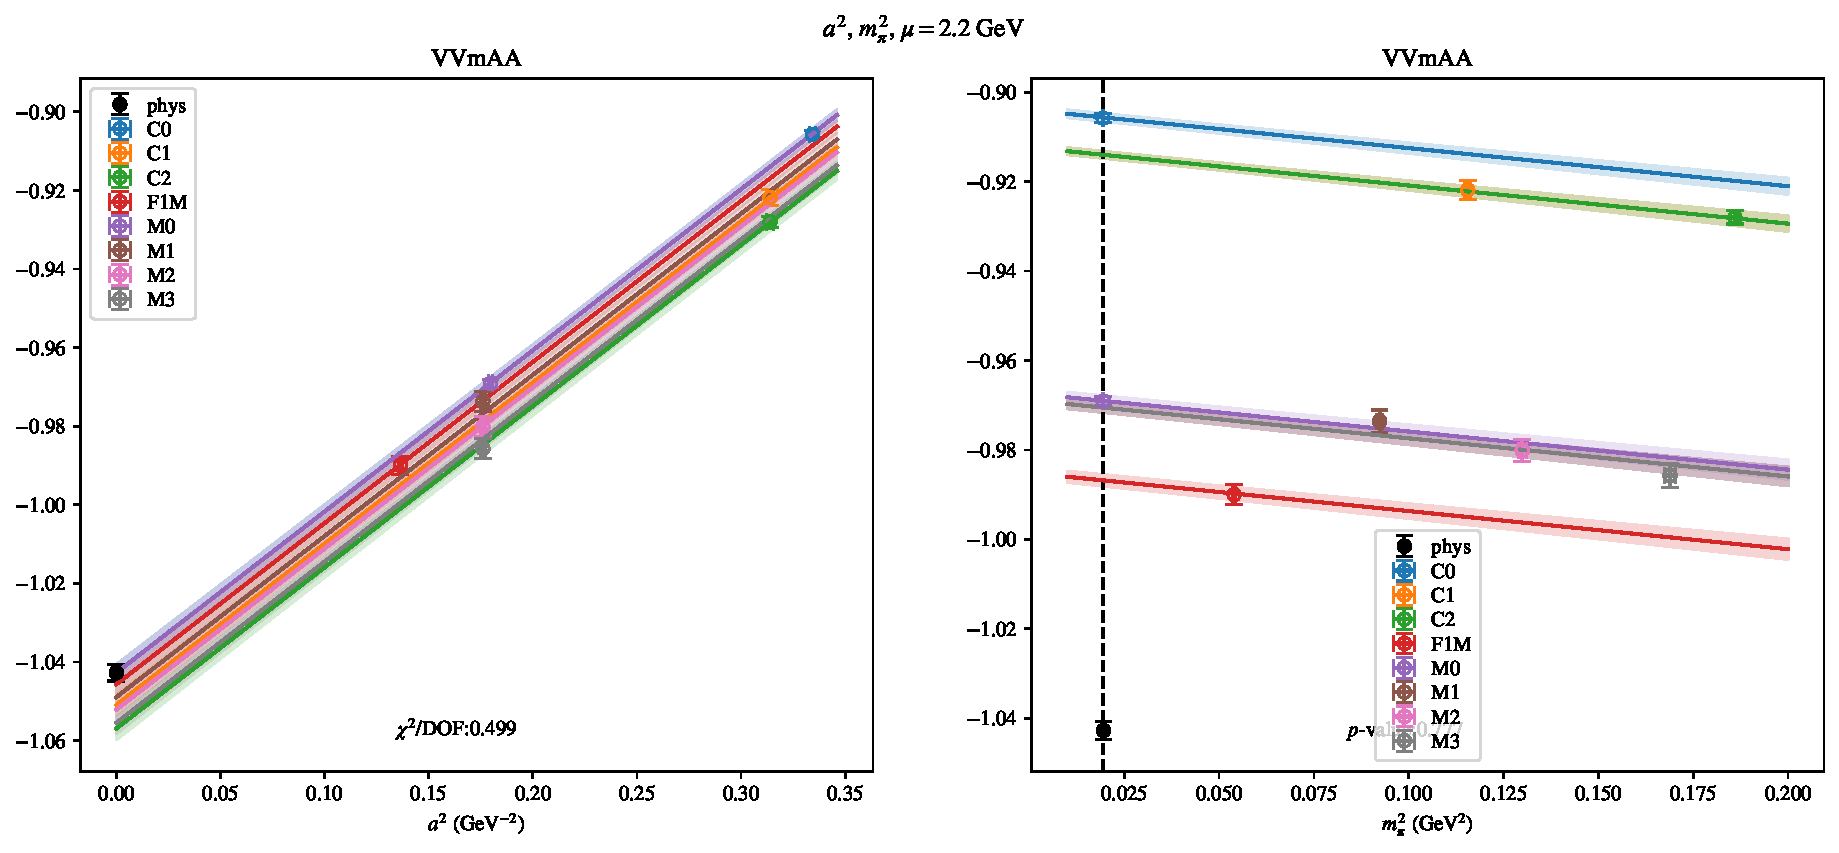
\includepdf[link, pages=-]{VVmAA/NPR/a2m2_22.pdf}
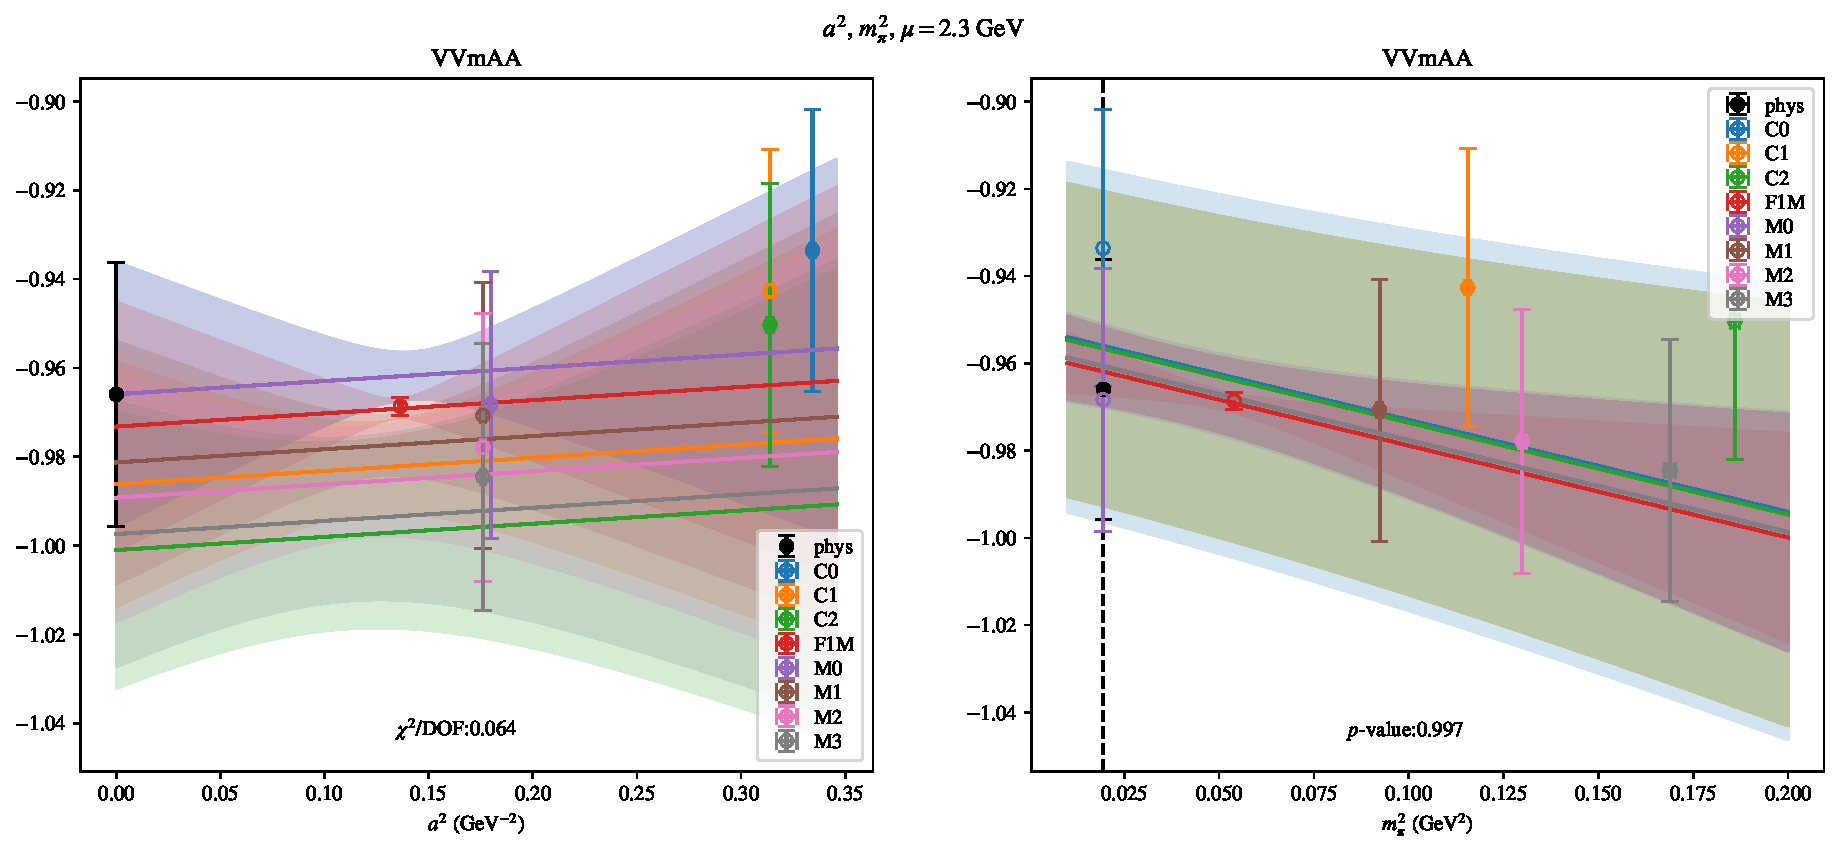
\includepdf[link, pages=-]{VVmAA/NPR/a2m2_23.pdf}
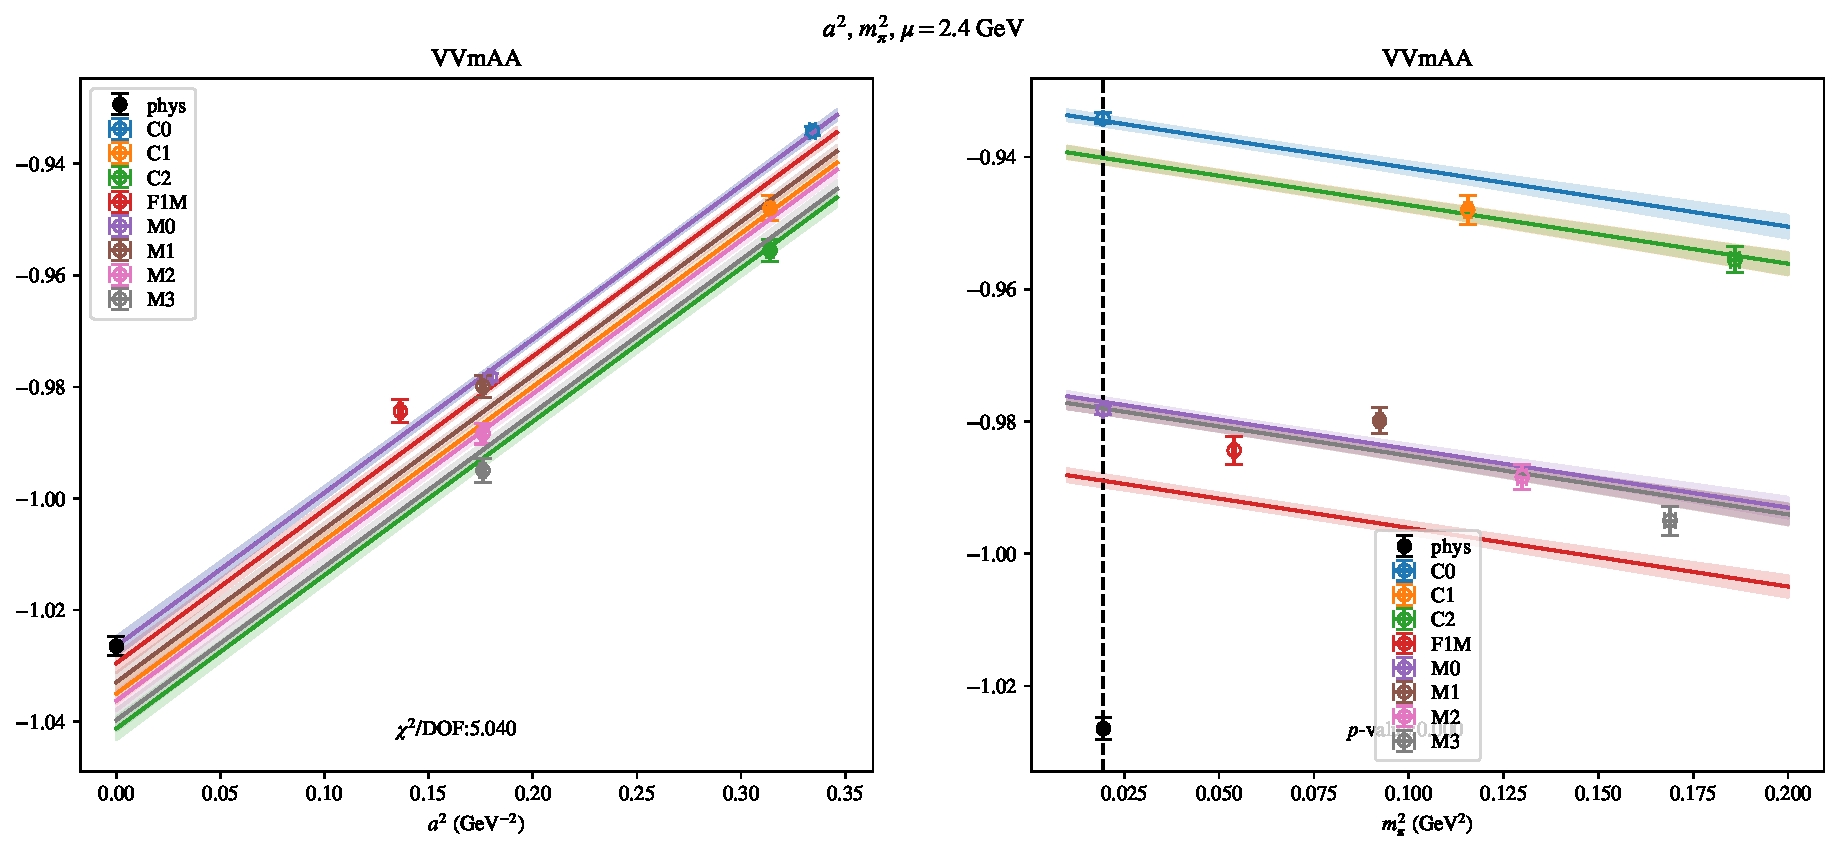
\includepdf[link, pages=-]{VVmAA/NPR/a2m2_24.pdf}
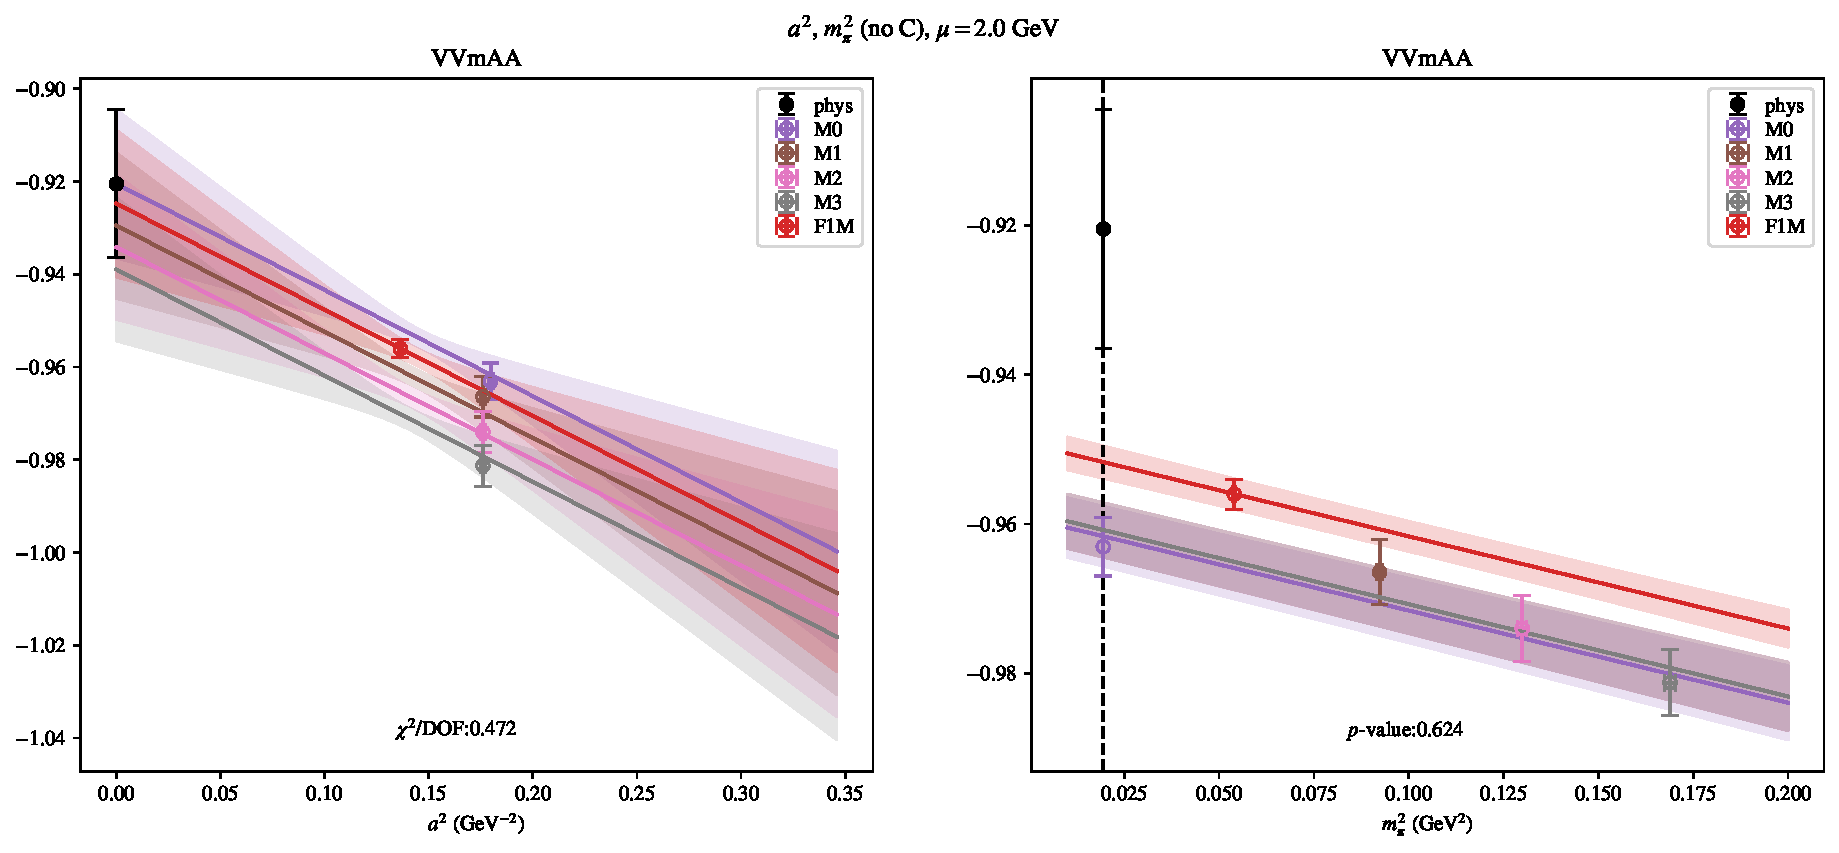
\includepdf[link, pages=-]{VVmAA/NPR/a2m2noC_20.pdf}
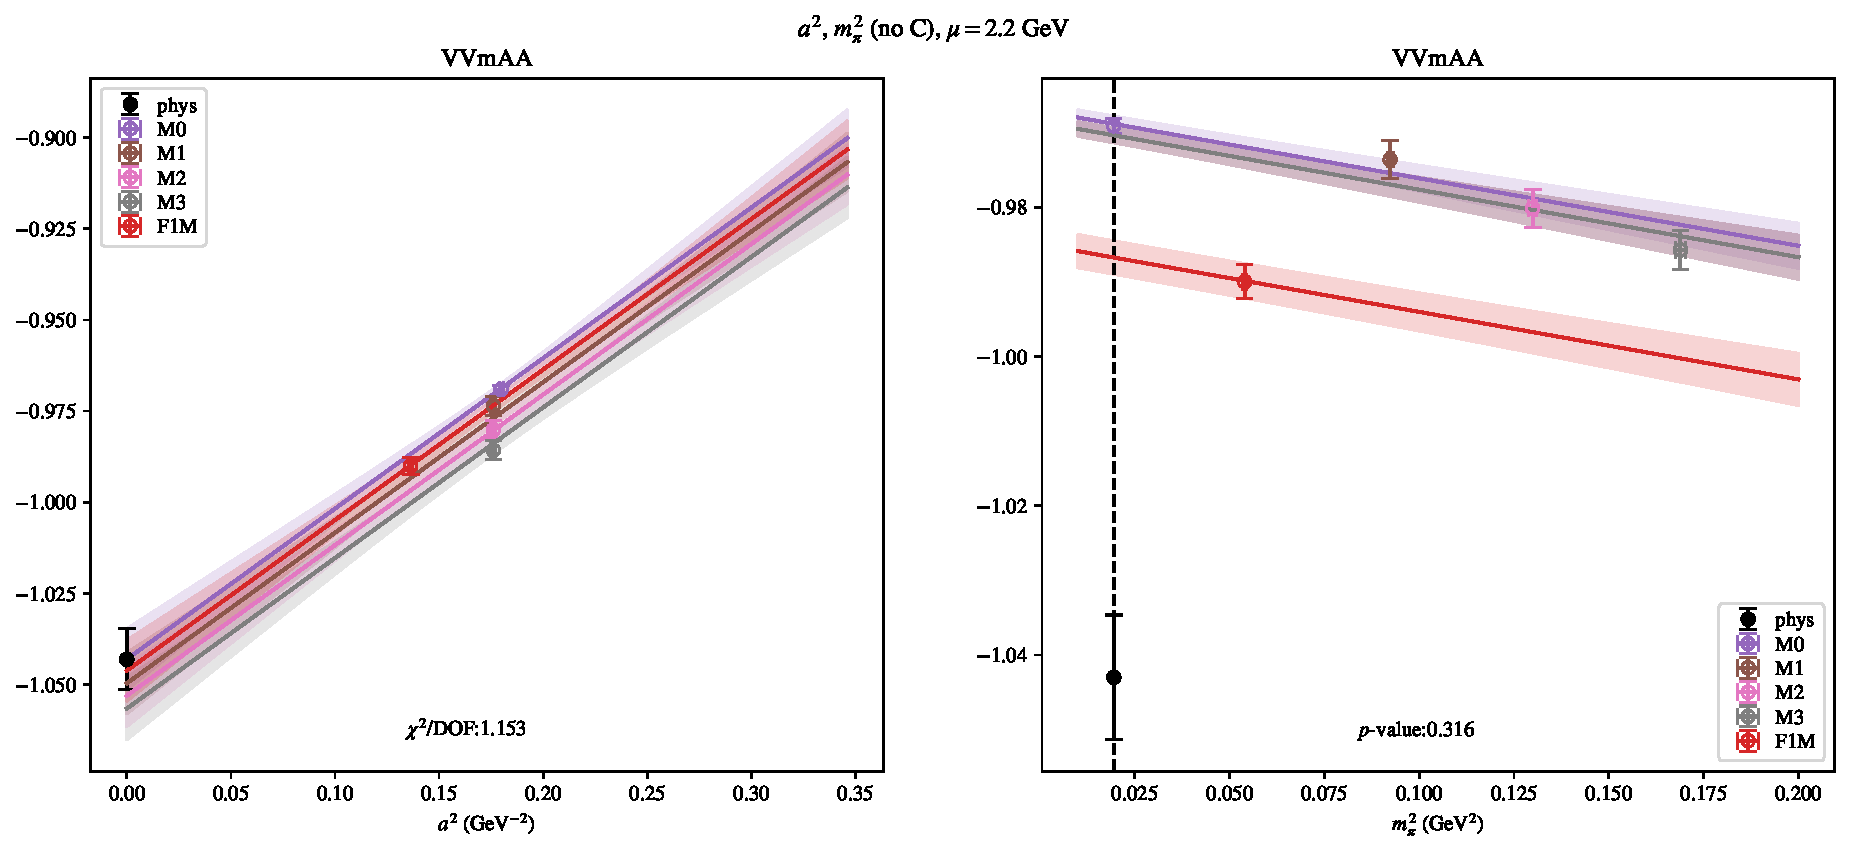
\includepdf[link, pages=-]{VVmAA/NPR/a2m2noC_22.pdf}
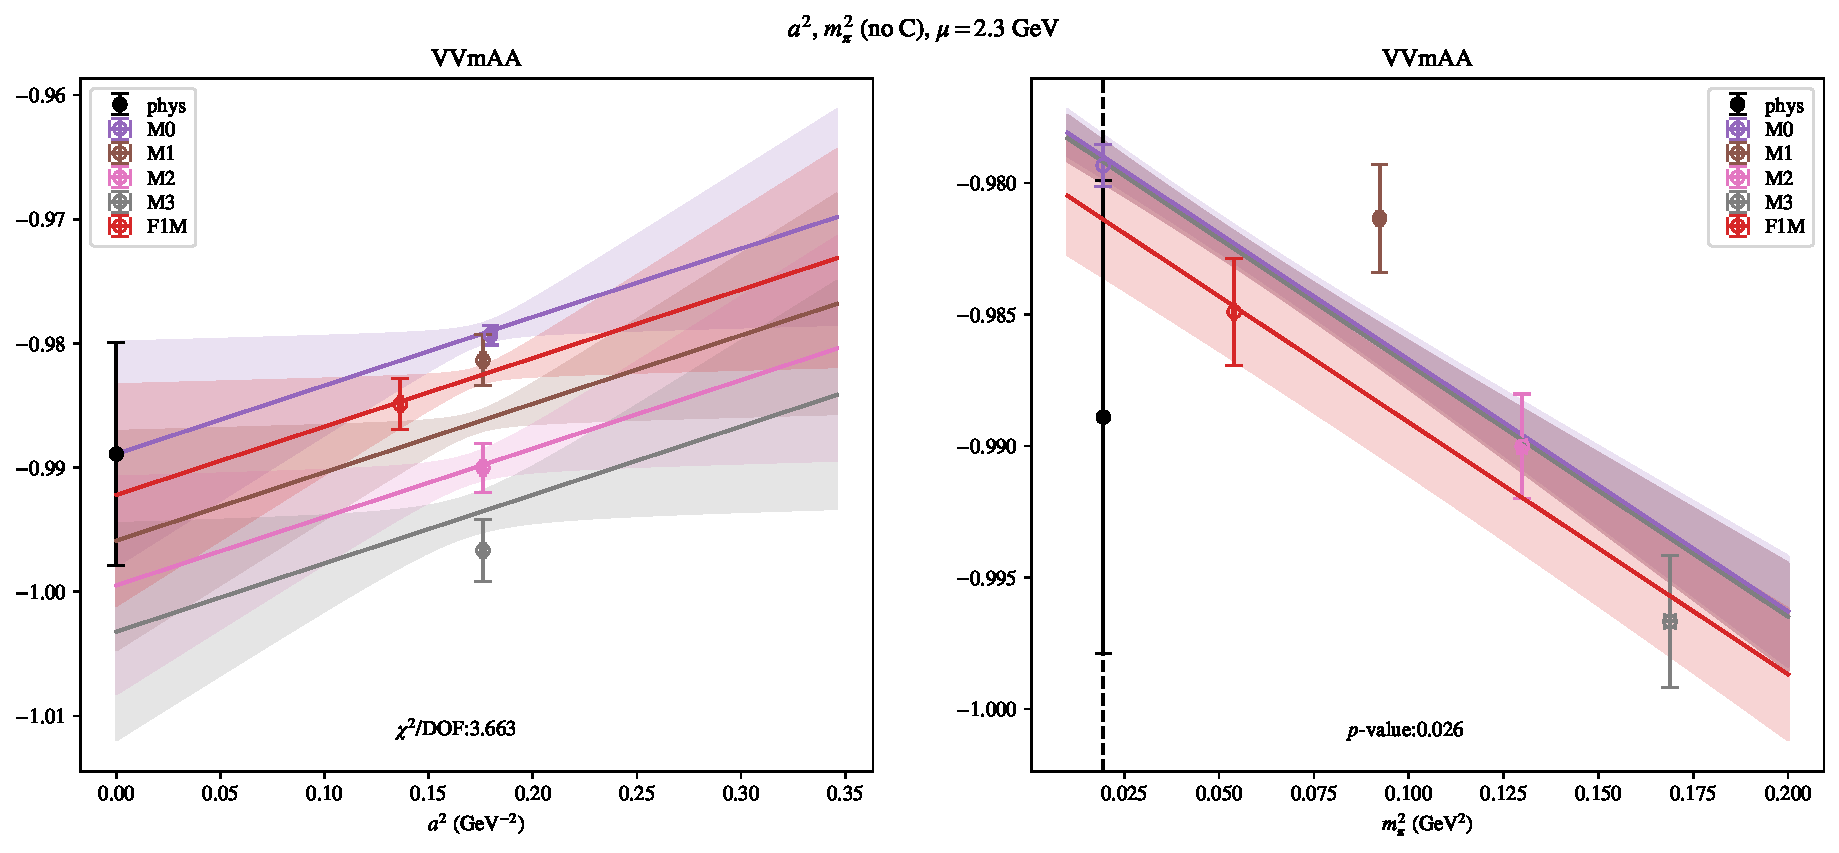
\includepdf[link, pages=-]{VVmAA/NPR/a2m2noC_23.pdf}
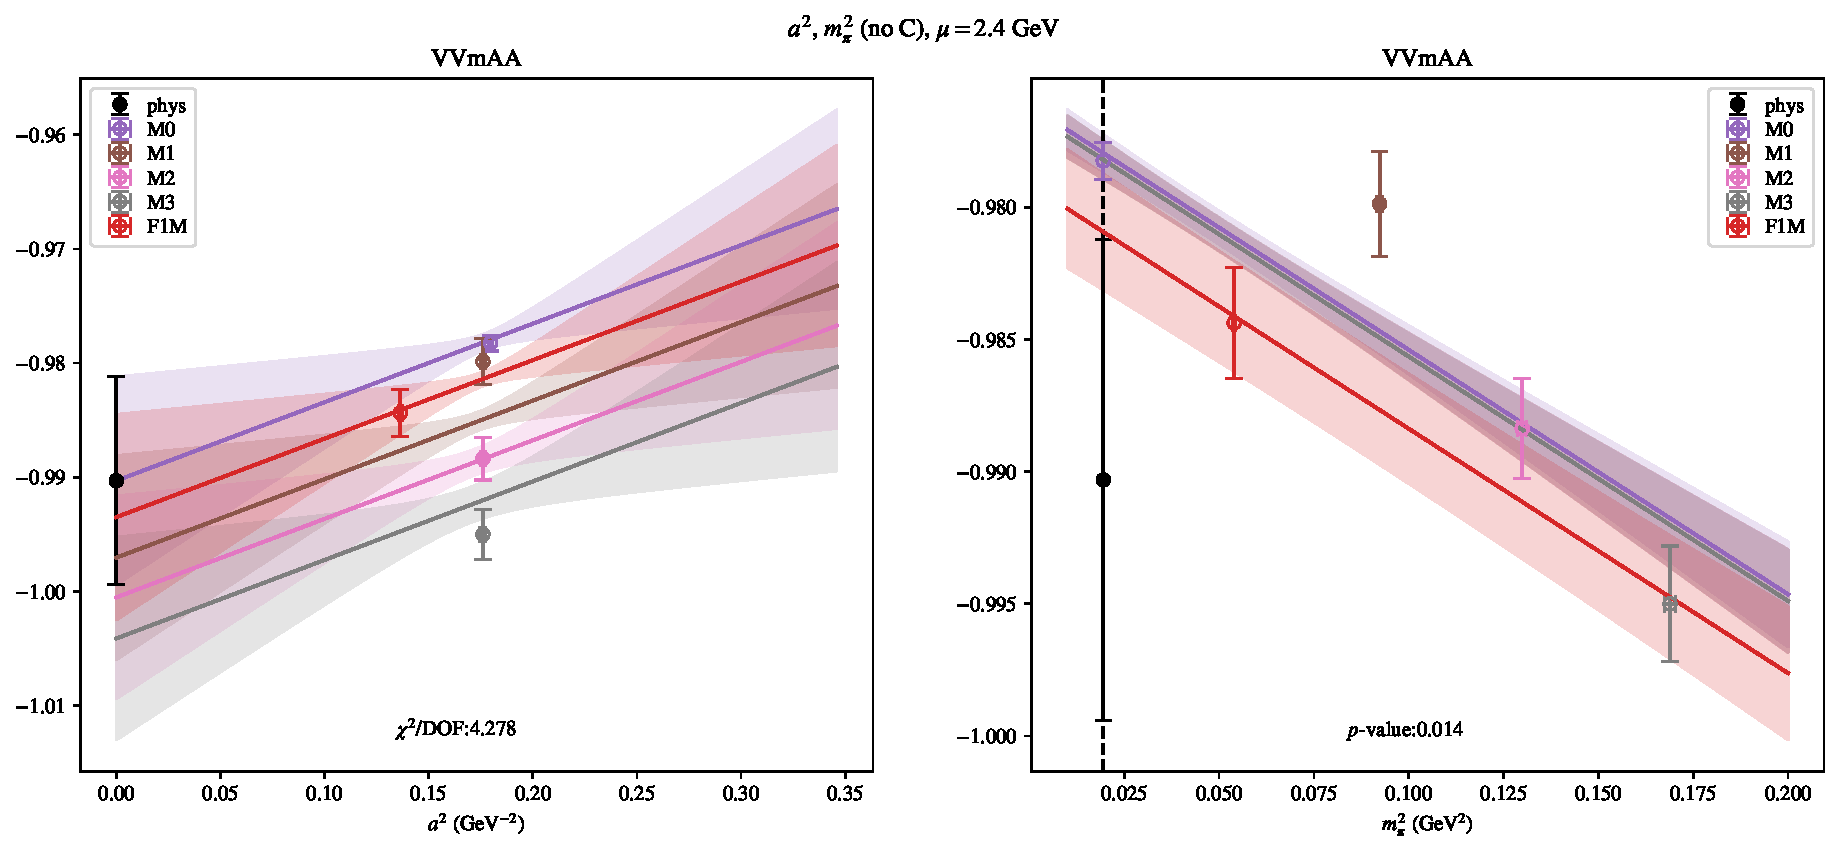
\includepdf[link, pages=-]{VVmAA/NPR/a2m2noC_24.pdf}
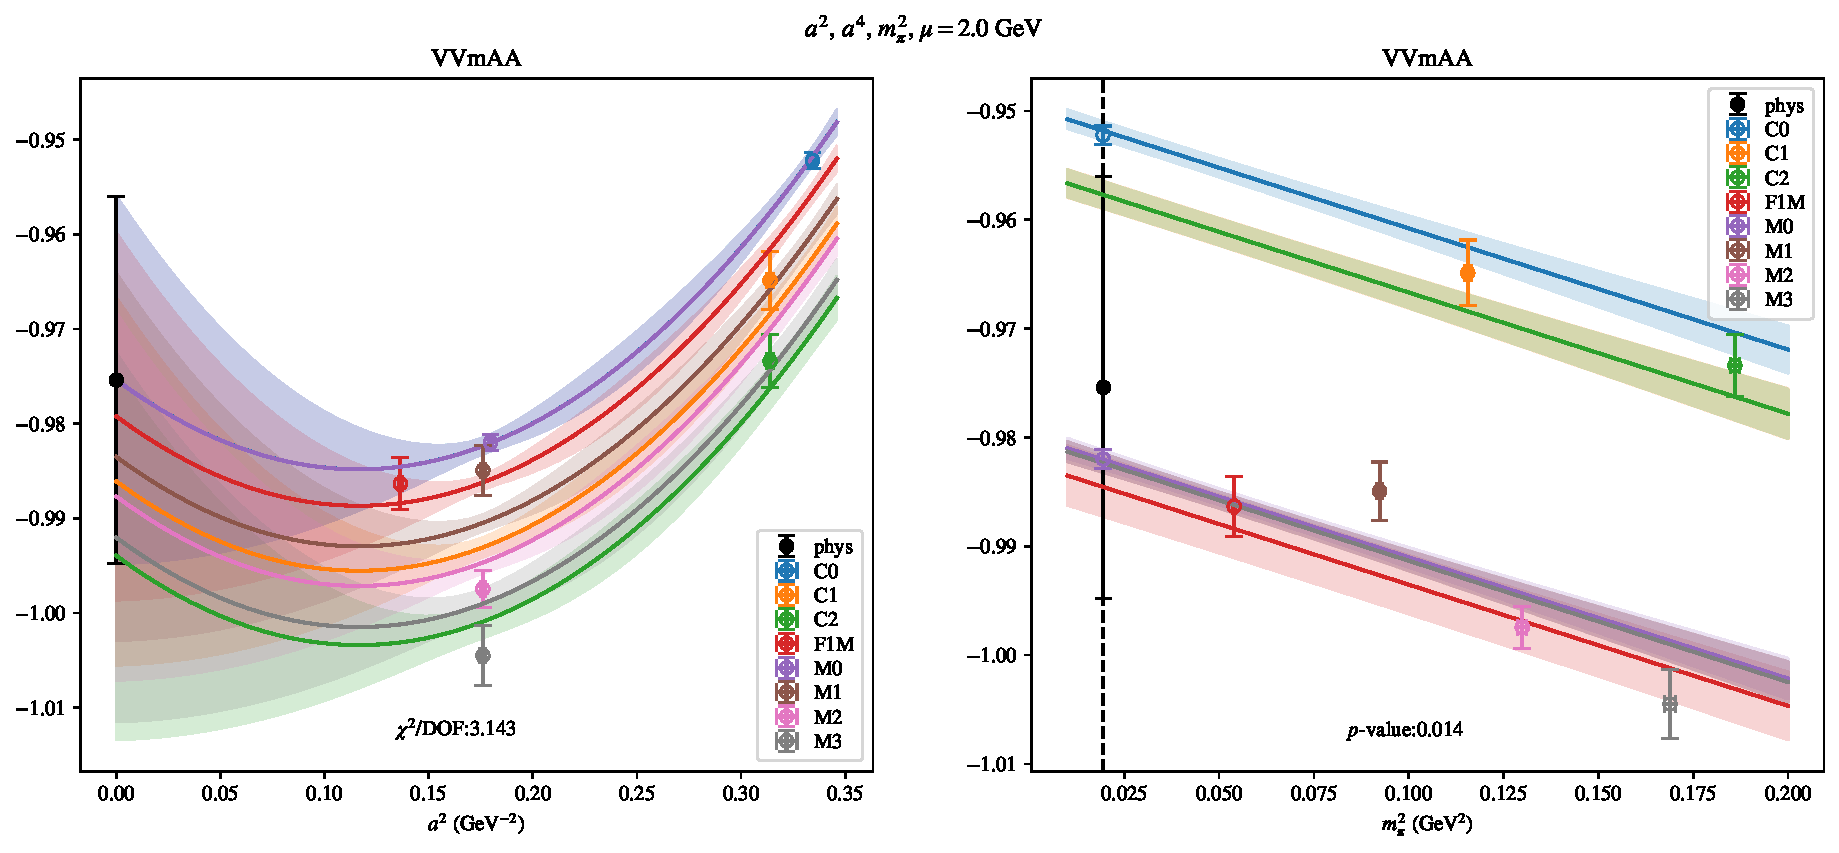
\includepdf[link, pages=-]{VVmAA/NPR/a2a4m2_20.pdf}
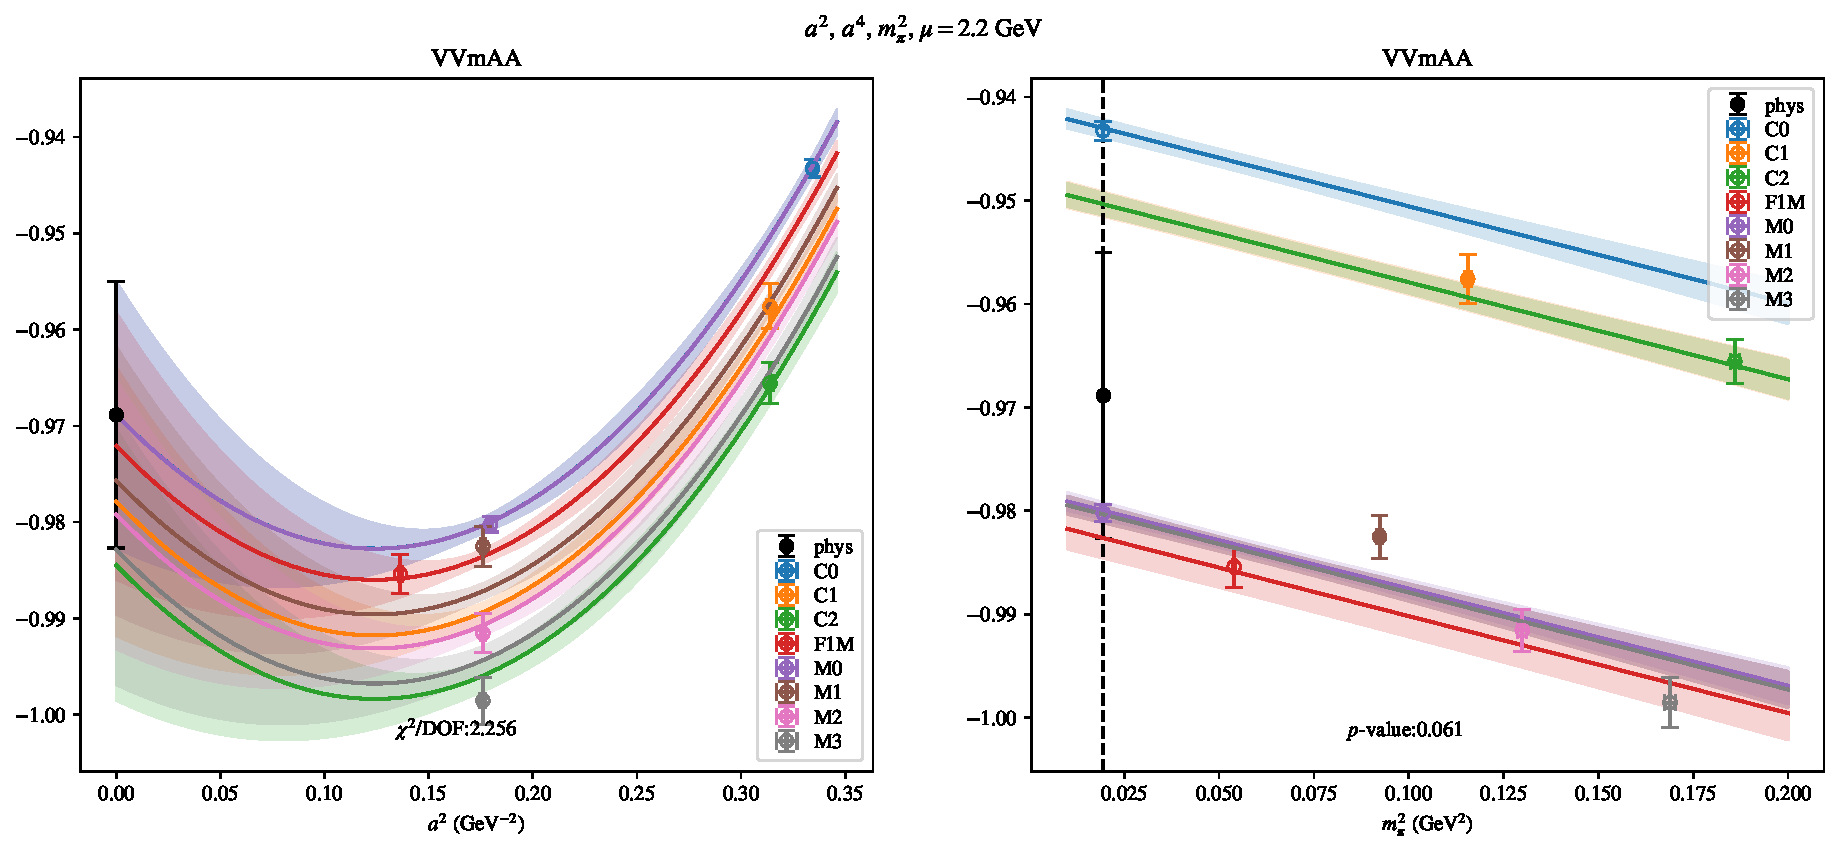
\includepdf[link, pages=-]{VVmAA/NPR/a2a4m2_22.pdf}
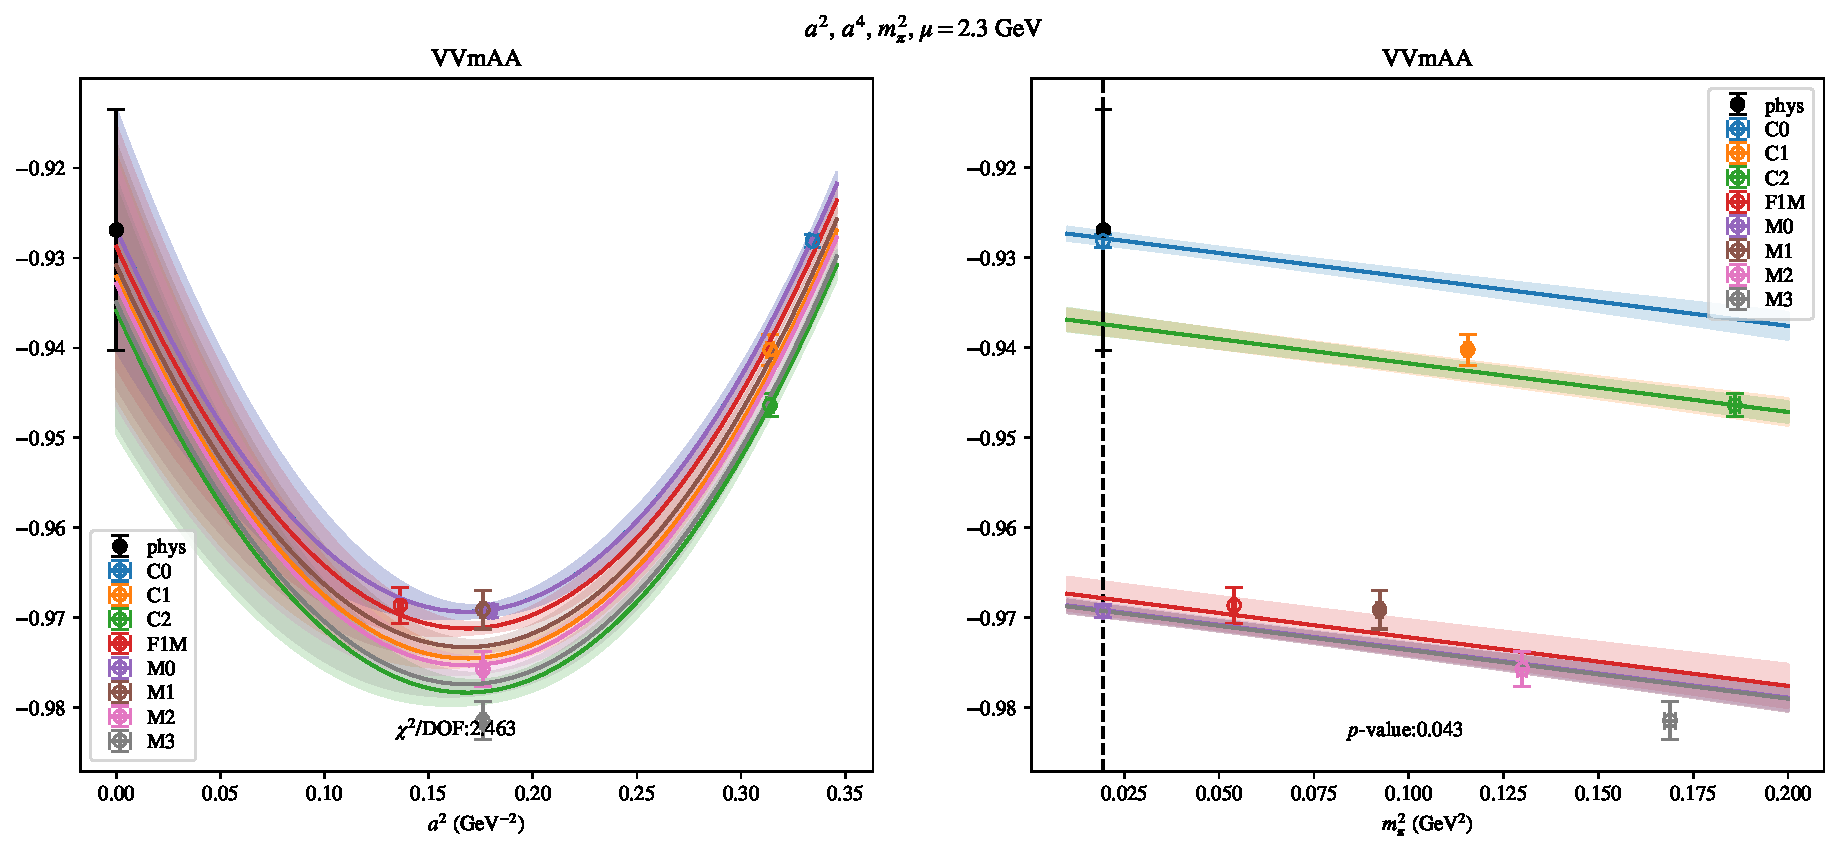
\includepdf[link, pages=-]{VVmAA/NPR/a2a4m2_23.pdf}
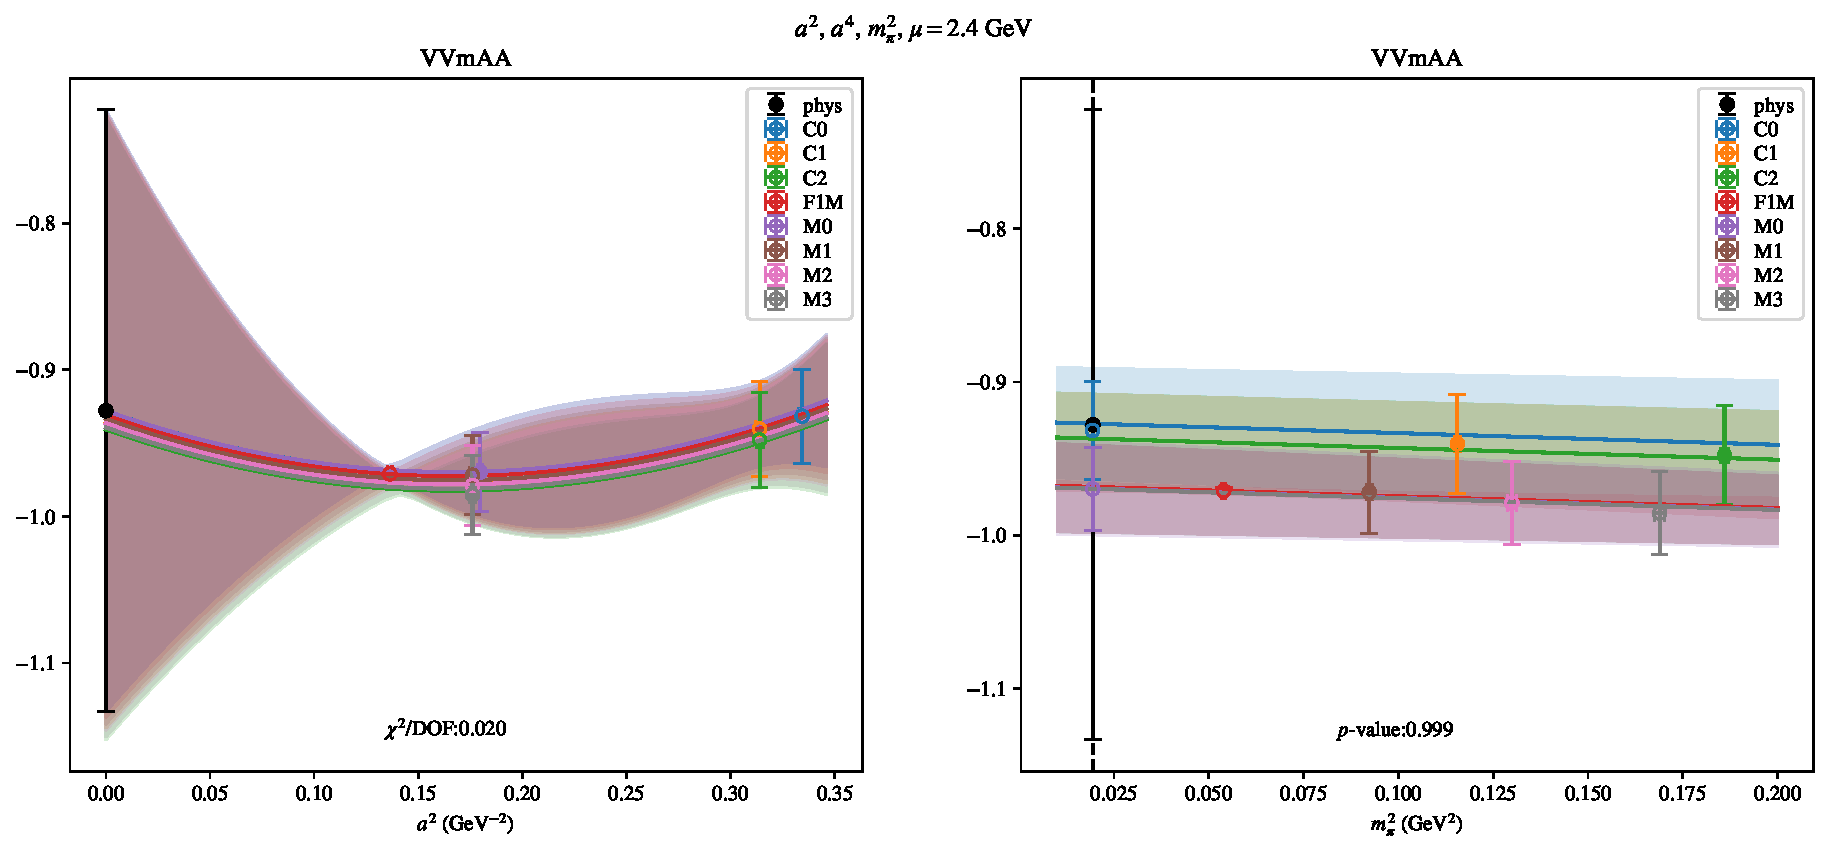
\includepdf[link, pages=-]{VVmAA/NPR/a2a4m2_24.pdf}
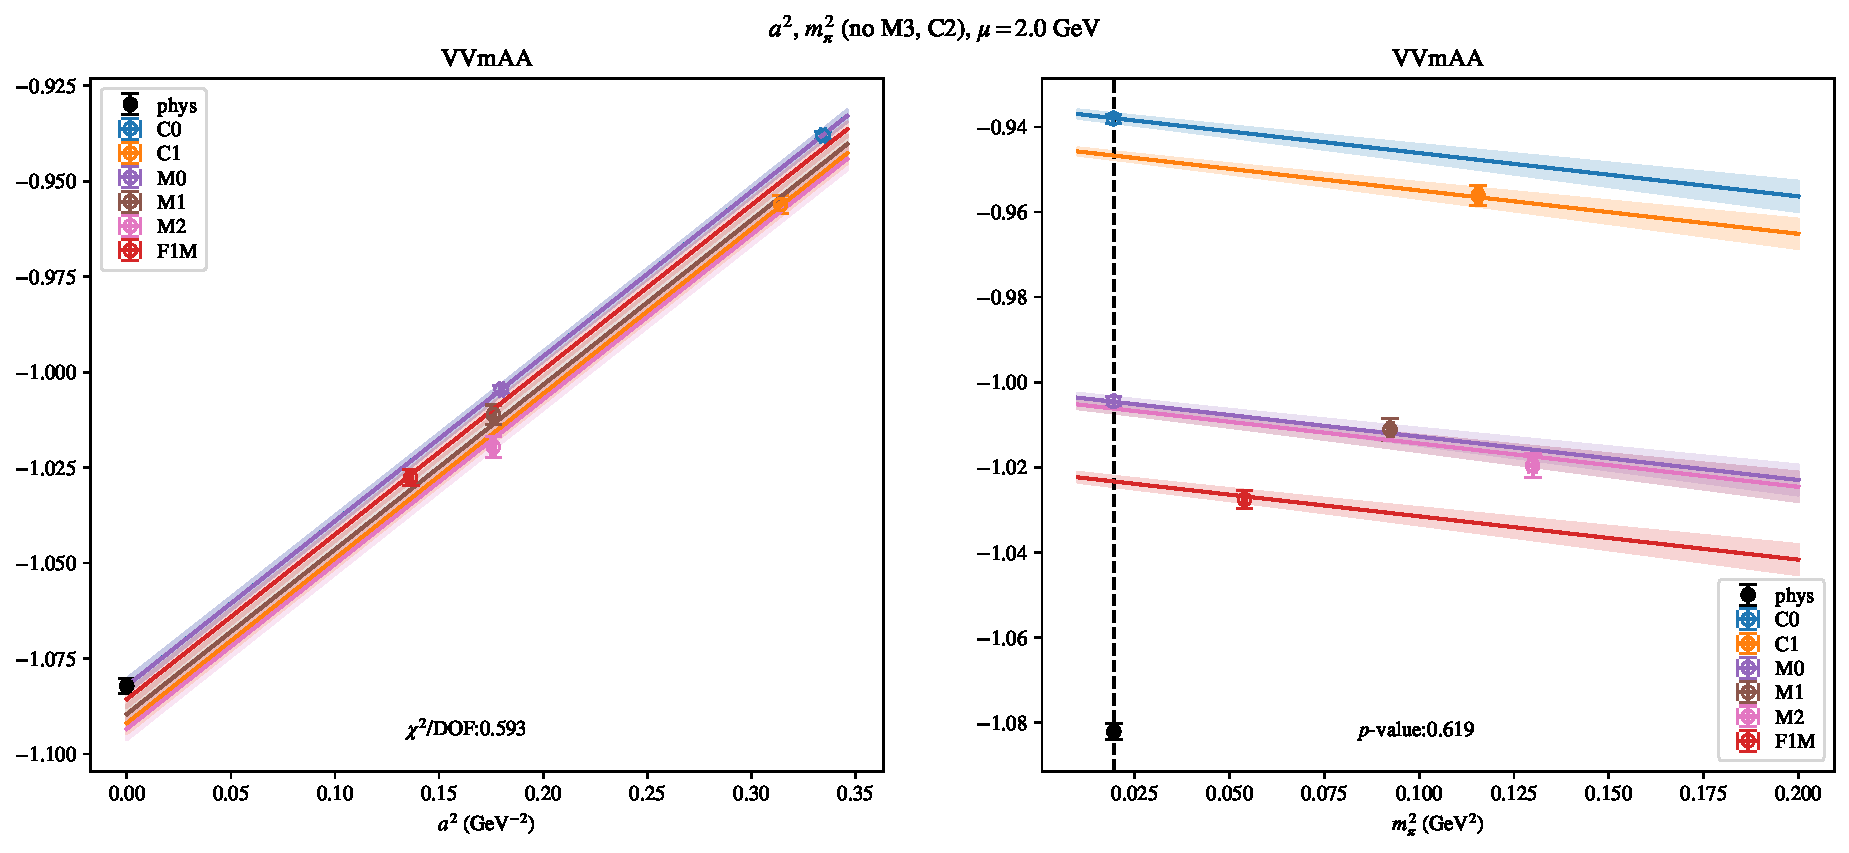
\includepdf[link, pages=-]{VVmAA/NPR/a2m2mcut_20.pdf}
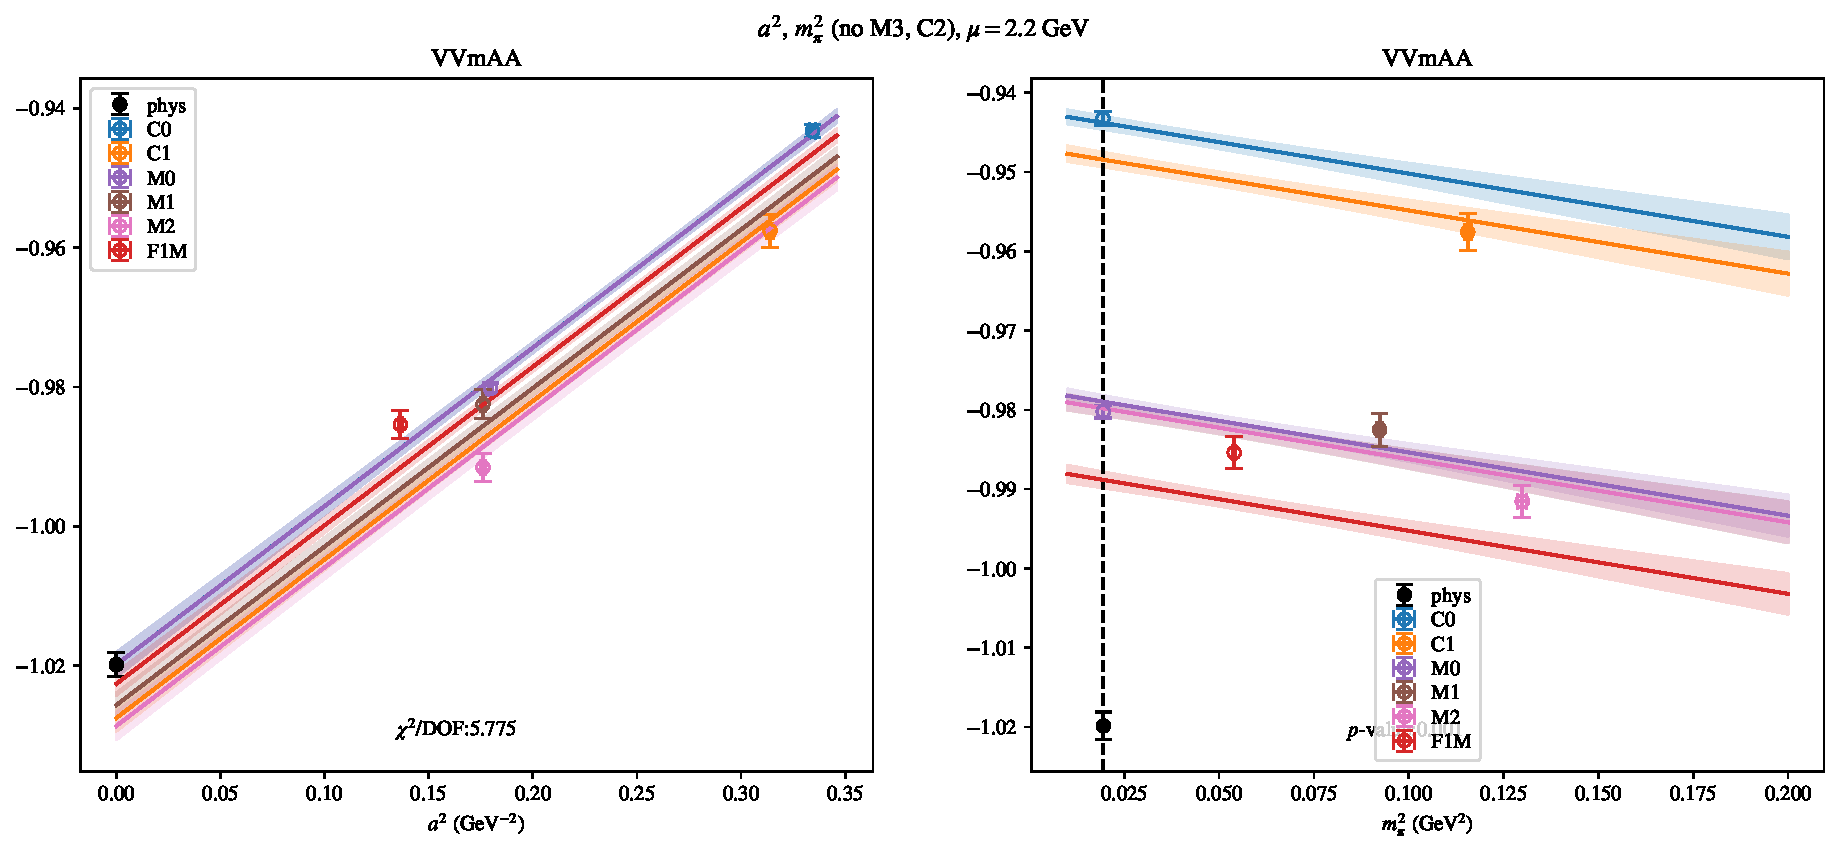
\includepdf[link, pages=-]{VVmAA/NPR/a2m2mcut_22.pdf}
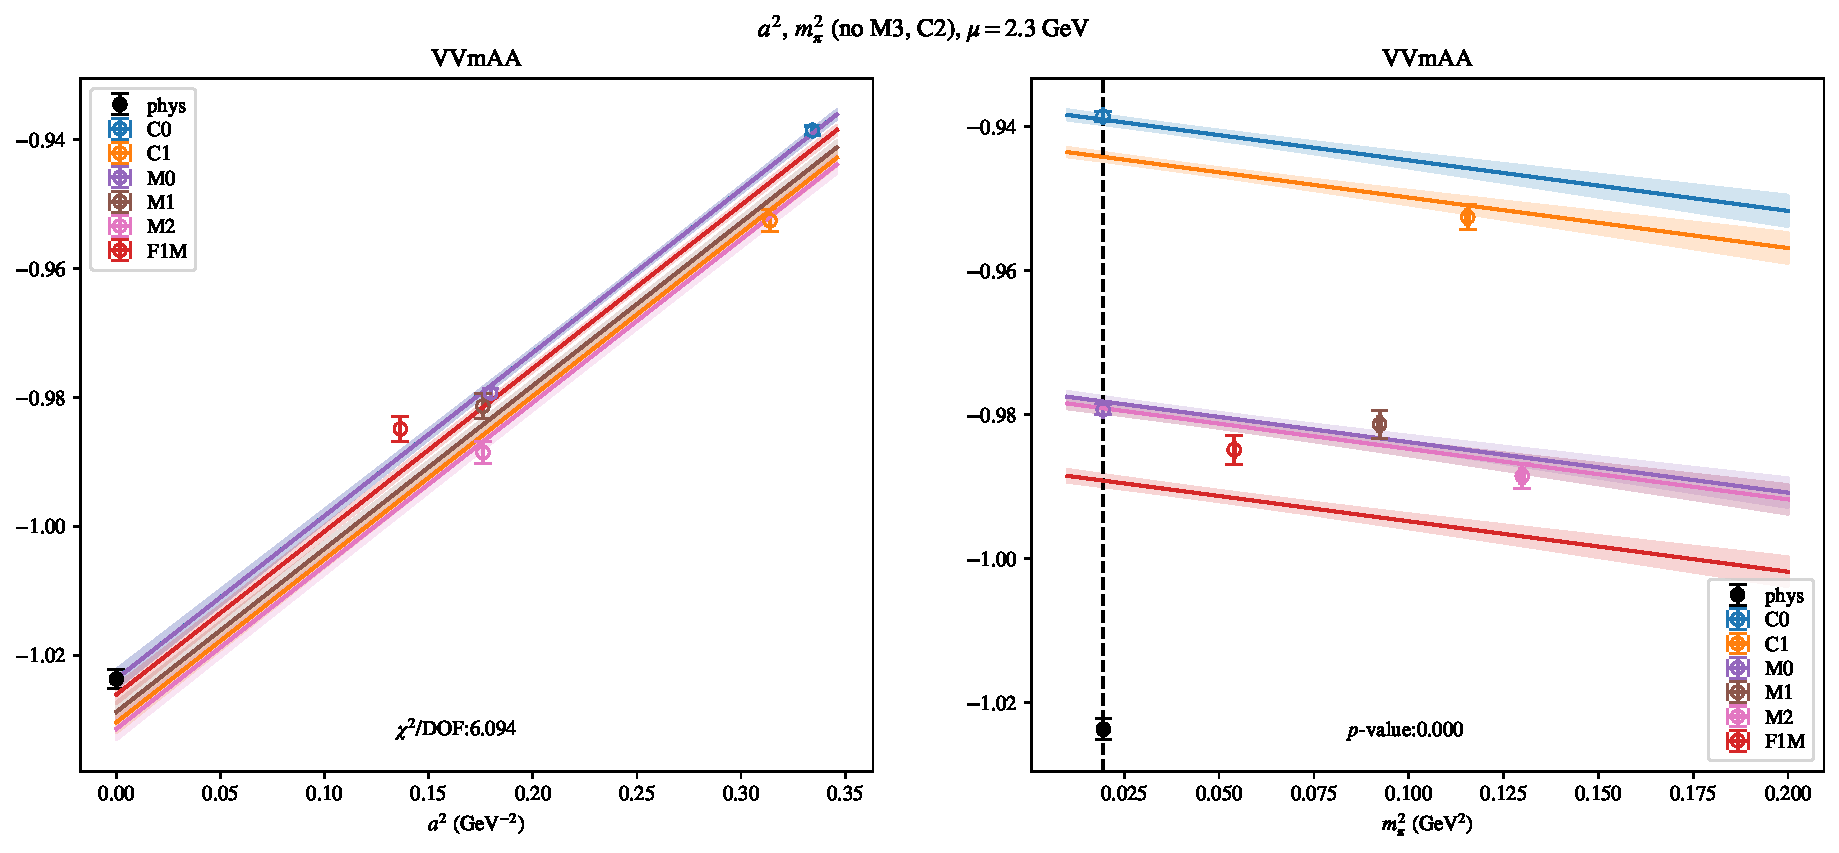
\includepdf[link, pages=-]{VVmAA/NPR/a2m2mcut_23.pdf}
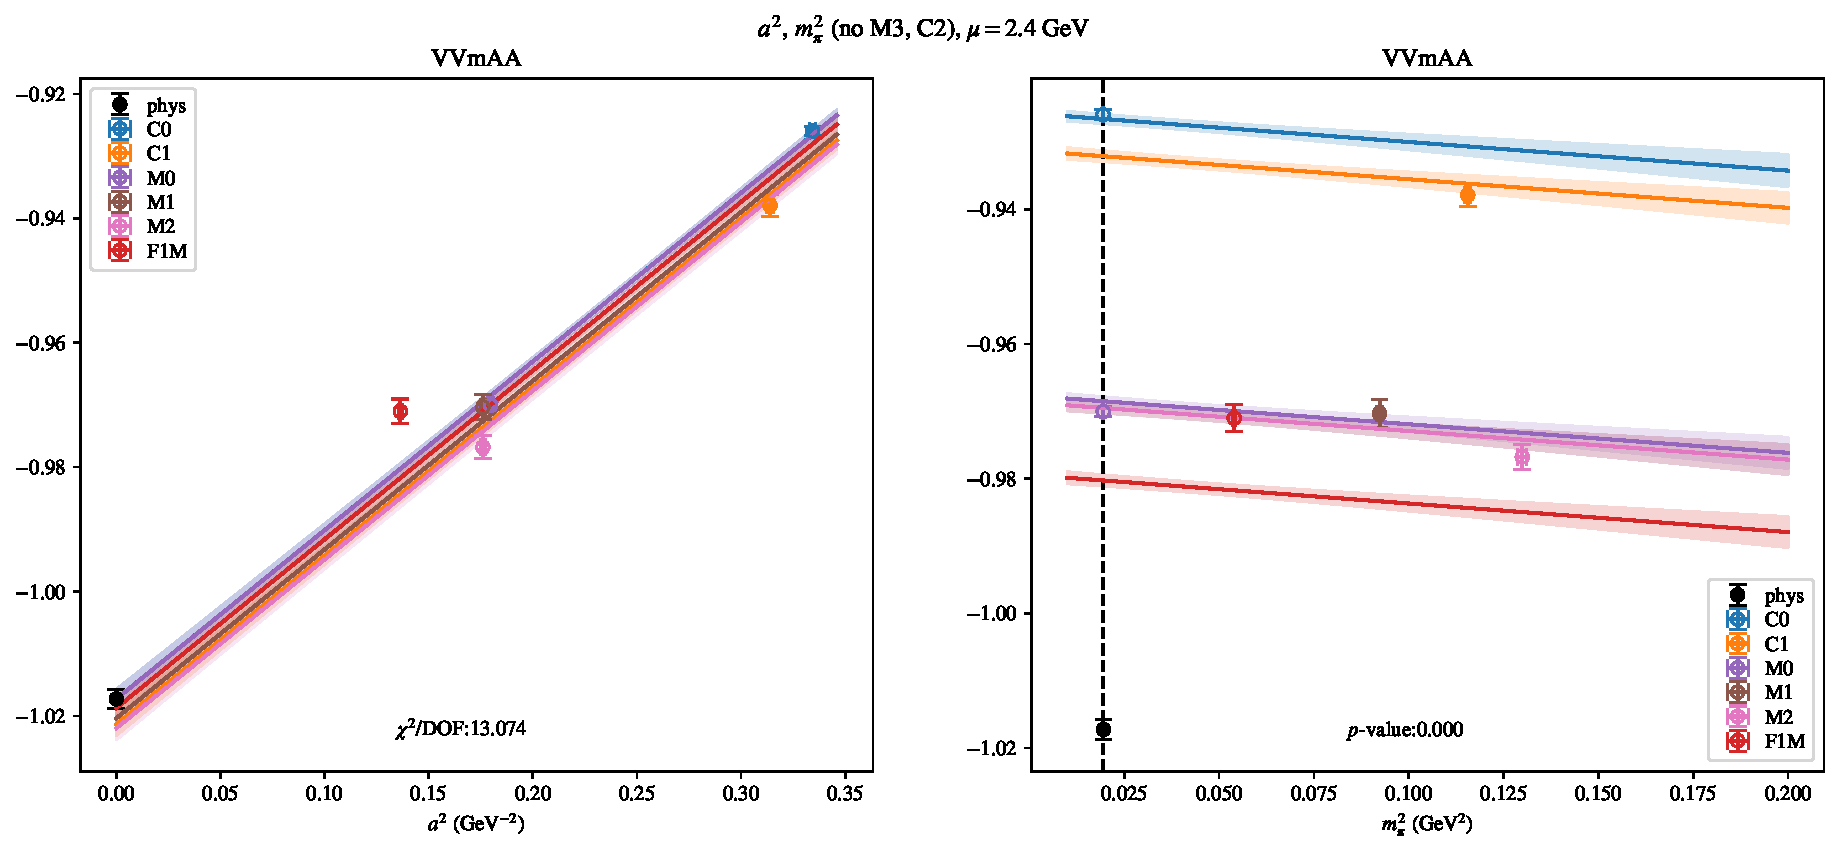
\includepdf[link, pages=-]{VVmAA/NPR/a2m2mcut_24.pdf}
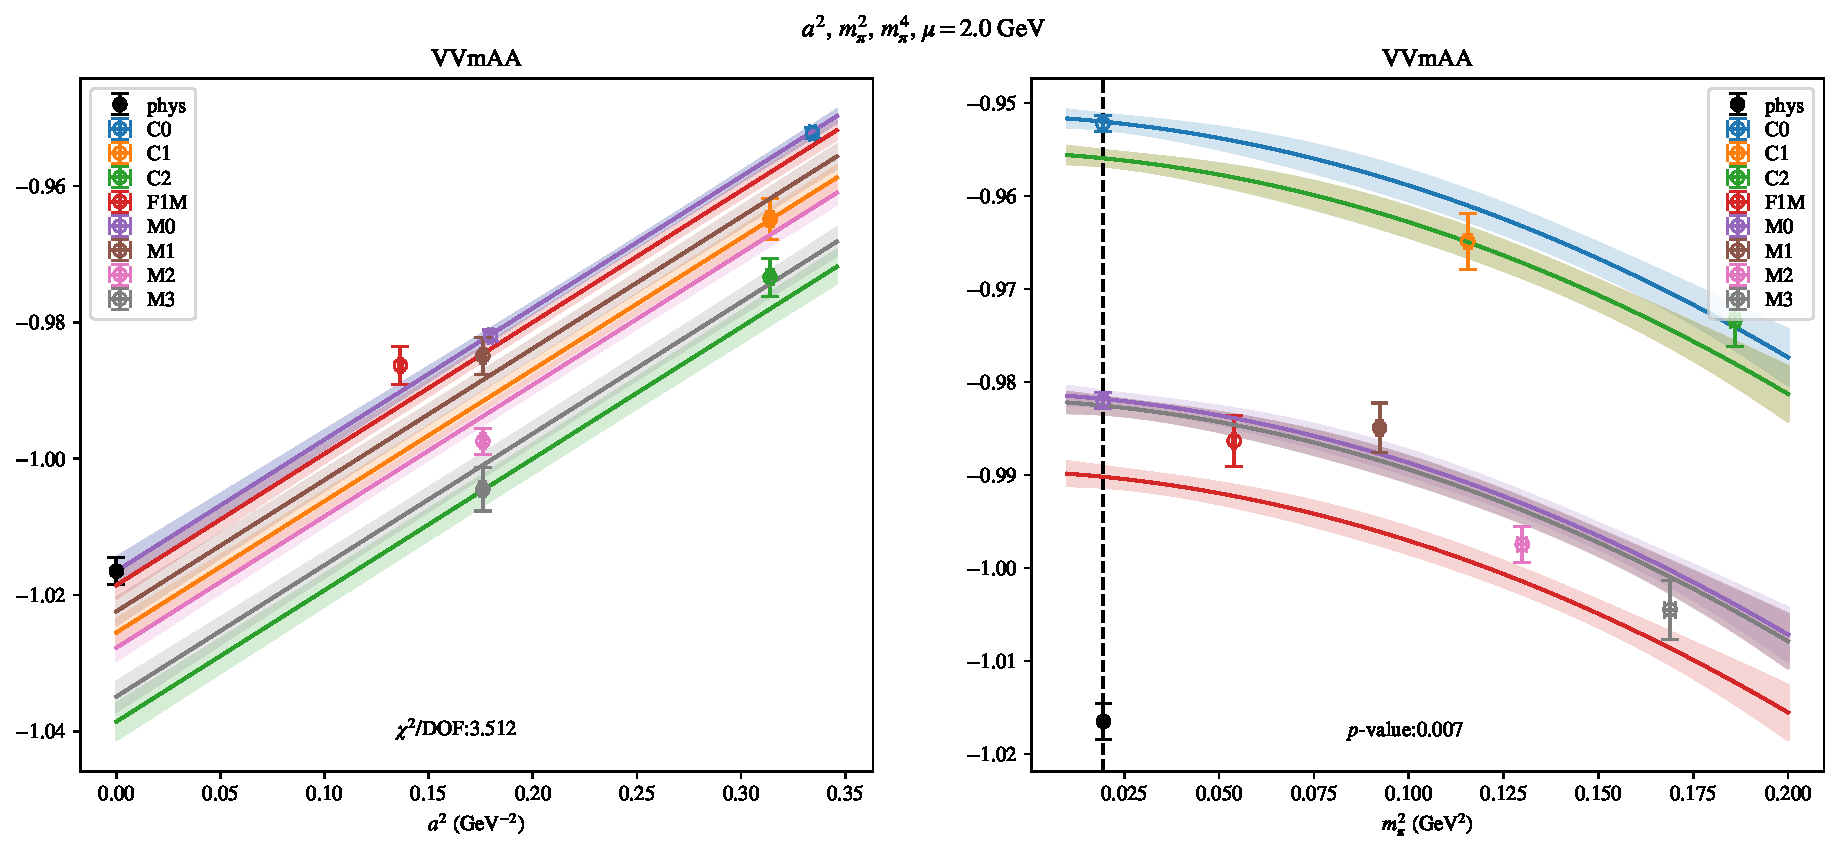
\includepdf[link, pages=-]{VVmAA/NPR/a2m2m4_20.pdf}
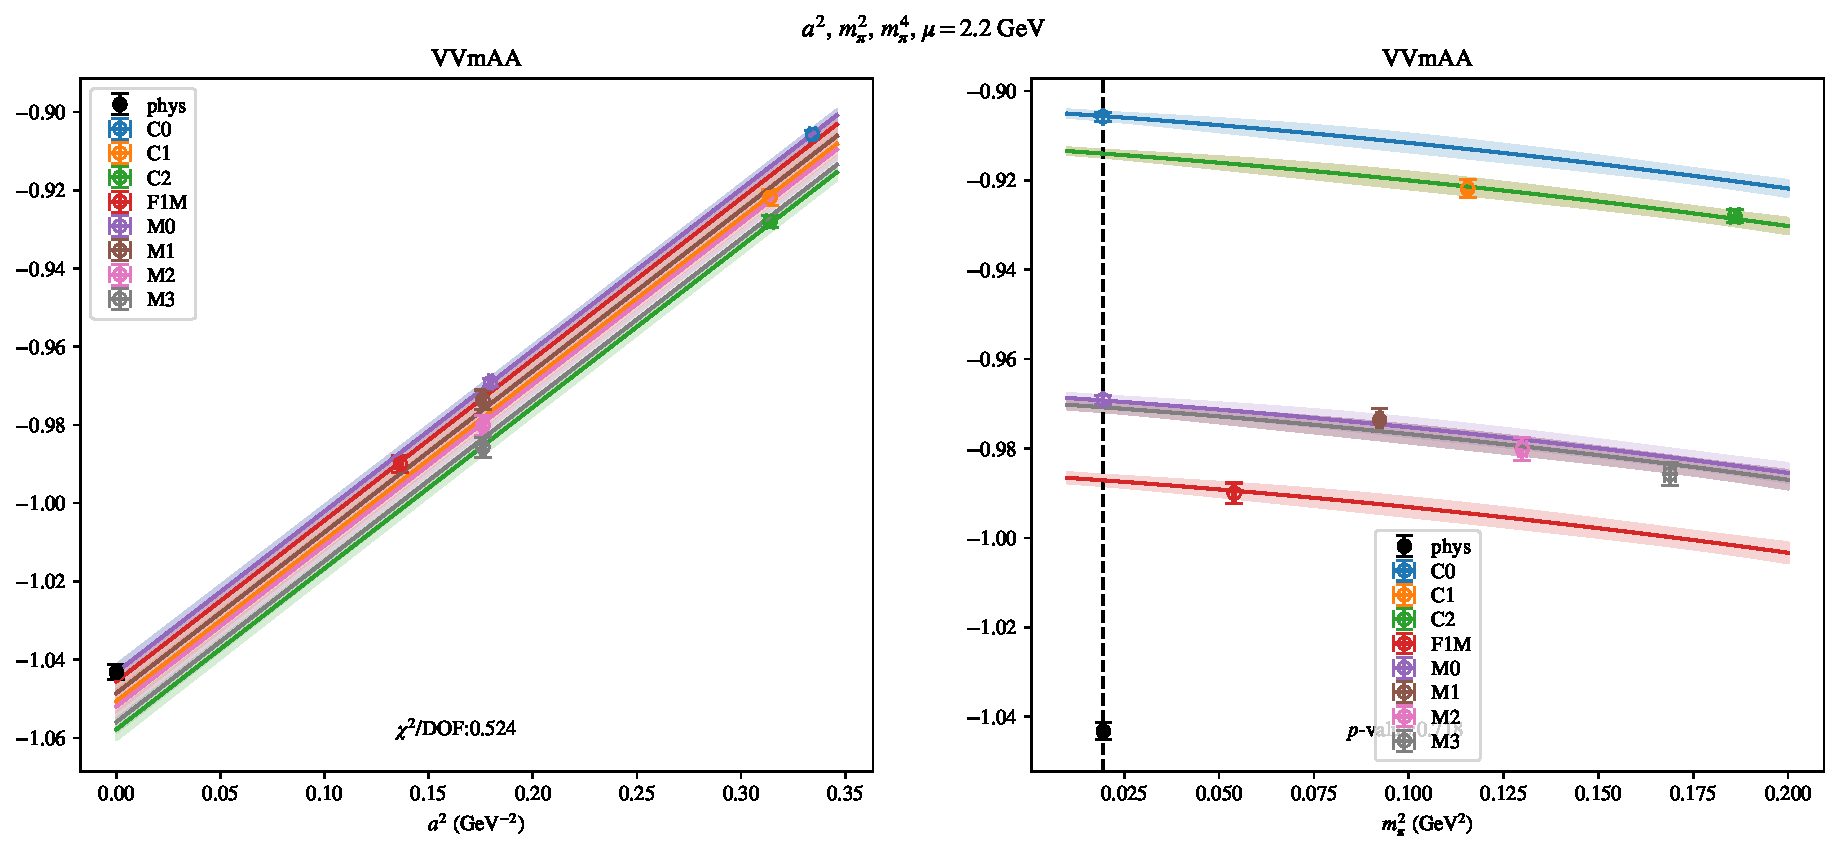
\includepdf[link, pages=-]{VVmAA/NPR/a2m2m4_22.pdf}
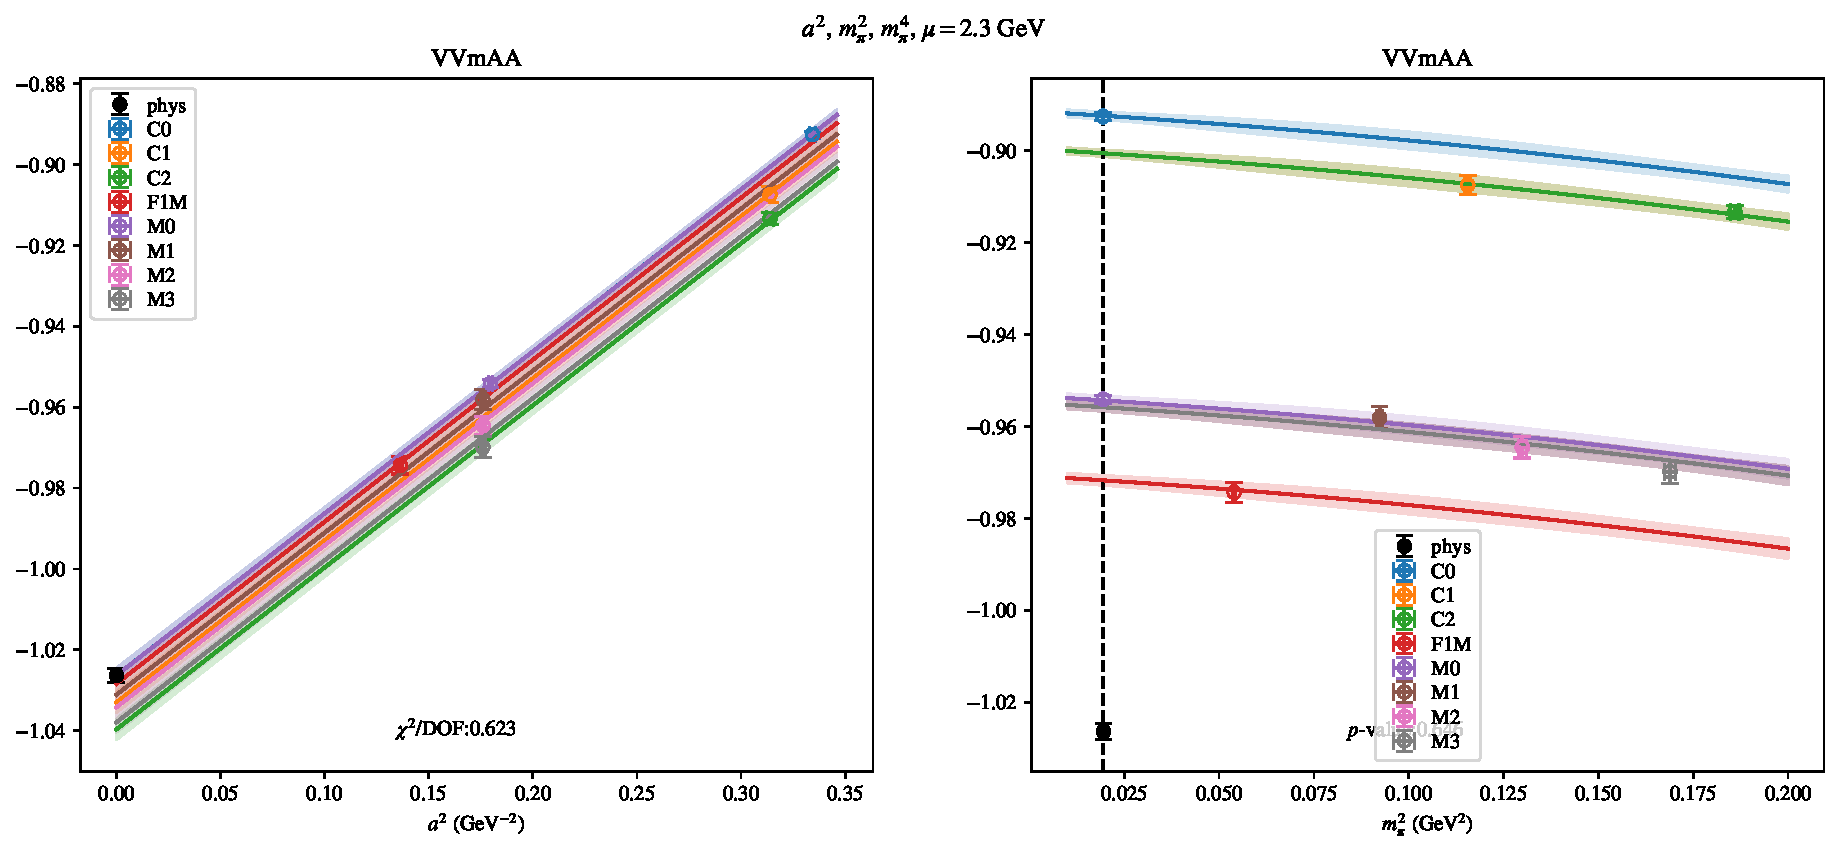
\includepdf[link, pages=-]{VVmAA/NPR/a2m2m4_23.pdf}
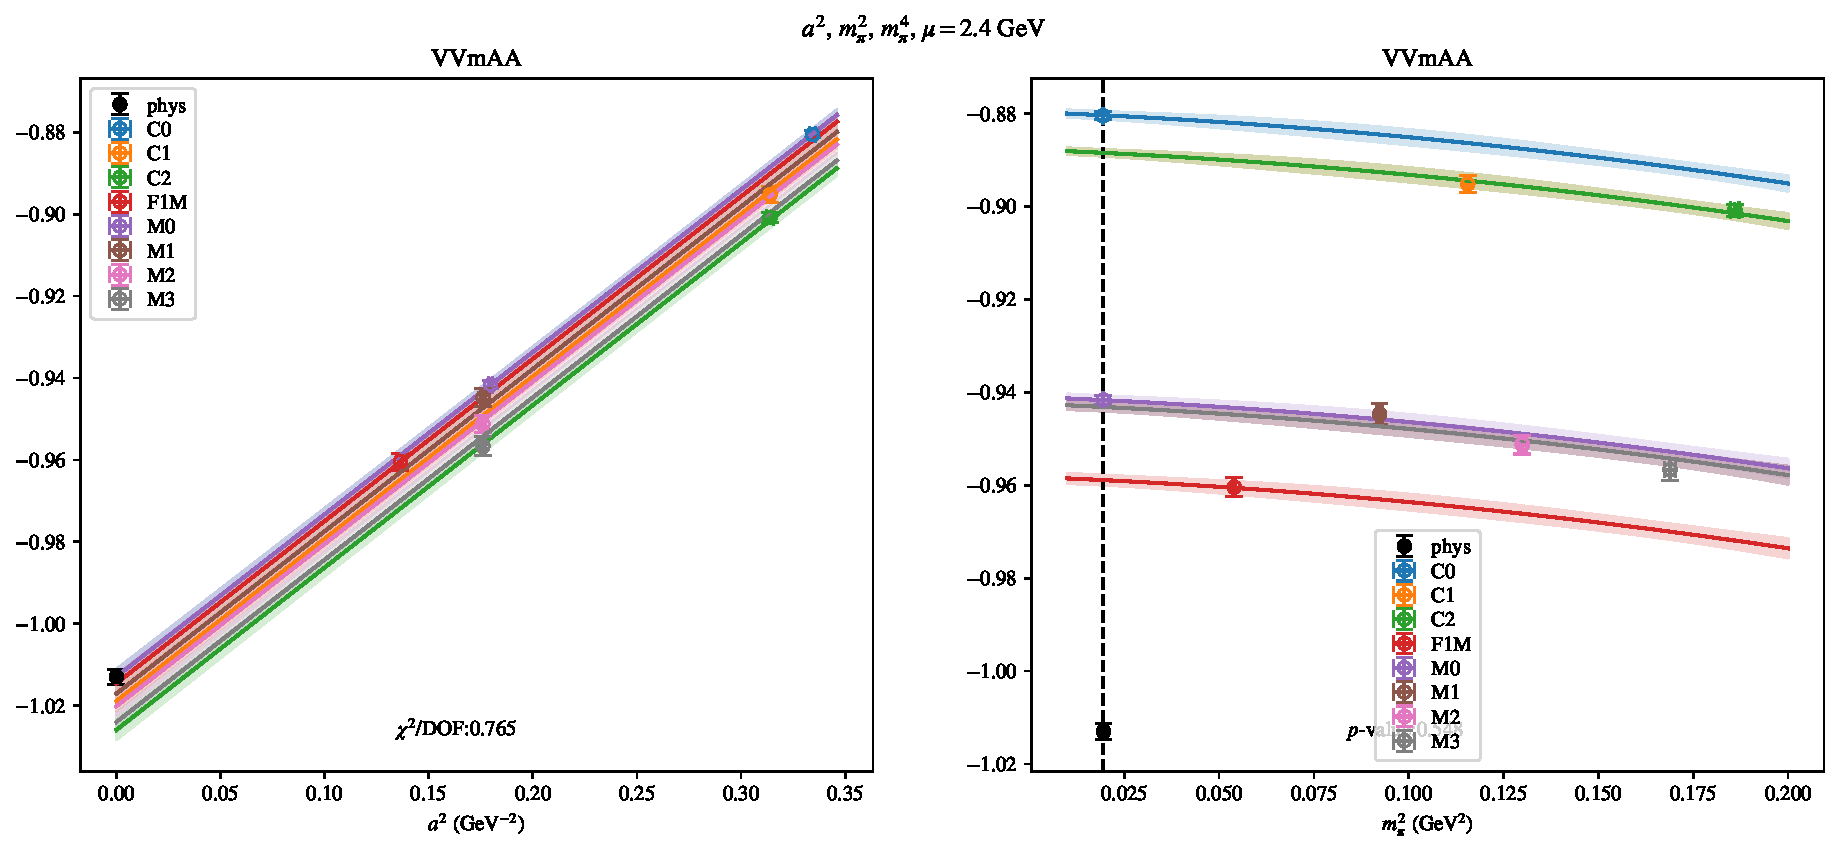
\includepdf[link, pages=-]{VVmAA/NPR/a2m2m4_24.pdf}
\clearpage
\section{$\mathcal{B}_3$}
\begin{table}[h!]
\begin{center}
\begin{tabular}{|c|c|c|c|c|c|}
\hline
$\mu$ (GeV) & $a^2$, $m_\pi^2$& $a^2$, $m_\pi^2$ (no C)& $a^2$, $a^4$, $m_\pi^2$& $a^2$, $m_\pi^2$ (no M3, C2)& $a^2$, $m_\pi^2$, $m_\pi^4$\\
\hline
2.0& \hyperlink{SSmPP/NPR/a2m2_20.pdf.1}{\textbf{20(21)}: 31060.216 (0.0)} & \hyperlink{SSmPP/NPR/a2m2noC_20.pdf.1}{\textbf{-1(76)}: 41155.309 (0.0)} & \hyperlink{SSmPP/NPR/a2a4m2_20.pdf.1}{\textbf{1(15)}: 38817.401 (0.0)} & \hyperlink{SSmPP/NPR/a2m2mcut_20.pdf.1}{\textbf{33(44)}: 27003.395 (0.0)} & \hyperlink{SSmPP/NPR/a2m2m4_20.pdf.1}{\textbf{50(26)}: 9500.047 (0.0)}\\
2.2& \hyperlink{SSmPP/NPR/a2m2_22.pdf.1}{\textbf{20(21)}: 31282.243 (0.0)} & \hyperlink{SSmPP/NPR/a2m2noC_22.pdf.1}{\textbf{-1(76)}: 41492.919 (0.0)} & \hyperlink{SSmPP/NPR/a2a4m2_22.pdf.1}{\textbf{1(15)}: 39093.899 (0.0)} & \hyperlink{SSmPP/NPR/a2m2mcut_22.pdf.1}{\textbf{33(44)}: 27257.96 (0.0)} & \hyperlink{SSmPP/NPR/a2m2m4_22.pdf.1}{\textbf{49(26)}: 9581.59 (0.0)}\\
2.3& \hyperlink{SSmPP/NPR/a2m2_23.pdf.1}{\textbf{20(21)}: 31350.748 (0.0)} & \hyperlink{SSmPP/NPR/a2m2noC_23.pdf.1}{\textbf{-1(75)}: 41596.728 (0.0)} & \hyperlink{SSmPP/NPR/a2a4m2_23.pdf.1}{\textbf{1(15)}: 39178.917 (0.0)} & \hyperlink{SSmPP/NPR/a2m2mcut_23.pdf.1}{\textbf{33(44)}: 27321.407 (0.0)} & \hyperlink{SSmPP/NPR/a2m2m4_23.pdf.1}{\textbf{49(26)}: 9602.315 (0.0)}\\
2.4& \hyperlink{SSmPP/NPR/a2m2_24.pdf.1}{\textbf{20(21)}: 31392.56 (0.0)} & \hyperlink{SSmPP/NPR/a2m2noC_24.pdf.1}{\textbf{-1(75)}: 41674.24 (0.0)} & \hyperlink{SSmPP/NPR/a2a4m2_24.pdf.1}{\textbf{1(15)}: 39230.658 (0.0)} & \hyperlink{SSmPP/NPR/a2m2mcut_24.pdf.1}{\textbf{33(44)}: 27358.42 (0.0)} & \hyperlink{SSmPP/NPR/a2m2m4_24.pdf.1}{\textbf{49(26)}: 9613.078 (0.0)}\\
\hline
\end{tabular}
\caption{Physical point value from chiral and continuum extrapolation at renormalisation scale $\mu$. Entries are \textbf{value(error)}: $\chi^2/\text{DOF}$ ($p$-value).}
\end{center}
\end{table}
\begin{table}[h!]
\begin{center}
\begin{tabular}{|c c|c|c|c|c|c|}
\hline
$\mu$ (GeV) &  & $a^2$, $m_\pi^2$& $a^2$, $m_\pi^2$ (no C)& $a^2$, $a^4$, $m_\pi^2$& $a^2$, $m_\pi^2$ (no M3, C2)& $a^2$, $m_\pi^2$, $m_\pi^4$\\
\hline
\multirow{2}{0.5in}{2.0} & $\alpha$ & 2.810(70)& -14.(31)& 7.5(20)& 1.976(78)& 0.667(19)\\
 & $\beta$ & -0.152(18)& 0.1623(54)& -0.21(26)& -0.205(28)& -0.344(18)\\
\hline
\multirow{2}{0.5in}{2.2} & $\alpha$ & 2.791(69)& -14.(31)& 7.8(21)& 1.961(77)& 0.663(19)\\
 & $\beta$ & -0.152(18)& 0.1613(54)& -0.21(28)& -0.204(28)& -0.344(18)\\
\hline
\multirow{2}{0.5in}{2.3} & $\alpha$ & 2.784(69)& -14.(31)& 8.0(21)& 1.957(77)& 0.662(19)\\
 & $\beta$ & -0.152(18)& 0.1607(53)& -0.22(28)& -0.204(28)& -0.343(18)\\
\hline
\multirow{2}{0.5in}{2.4} & $\alpha$ & 2.784(69)& -14.(30)& 8.2(22)& 1.956(77)& 0.663(19)\\
 & $\beta$ & -0.152(18)& 0.1603(53)& -0.22(29)& -0.204(28)& -0.344(18)\\
\hline
\end{tabular}
\caption{Fit values of coefficients in $Q = Q_{phys} + \mathbf{\alpha} a^2 + \mathbf{\beta}\left(\frac{m_\pi^2}{f_\pi^2}-\frac{m_{\pi,PDG}^2}{f_\pi^2}\right) + \ldots$.}
\end{center}
\end{table}
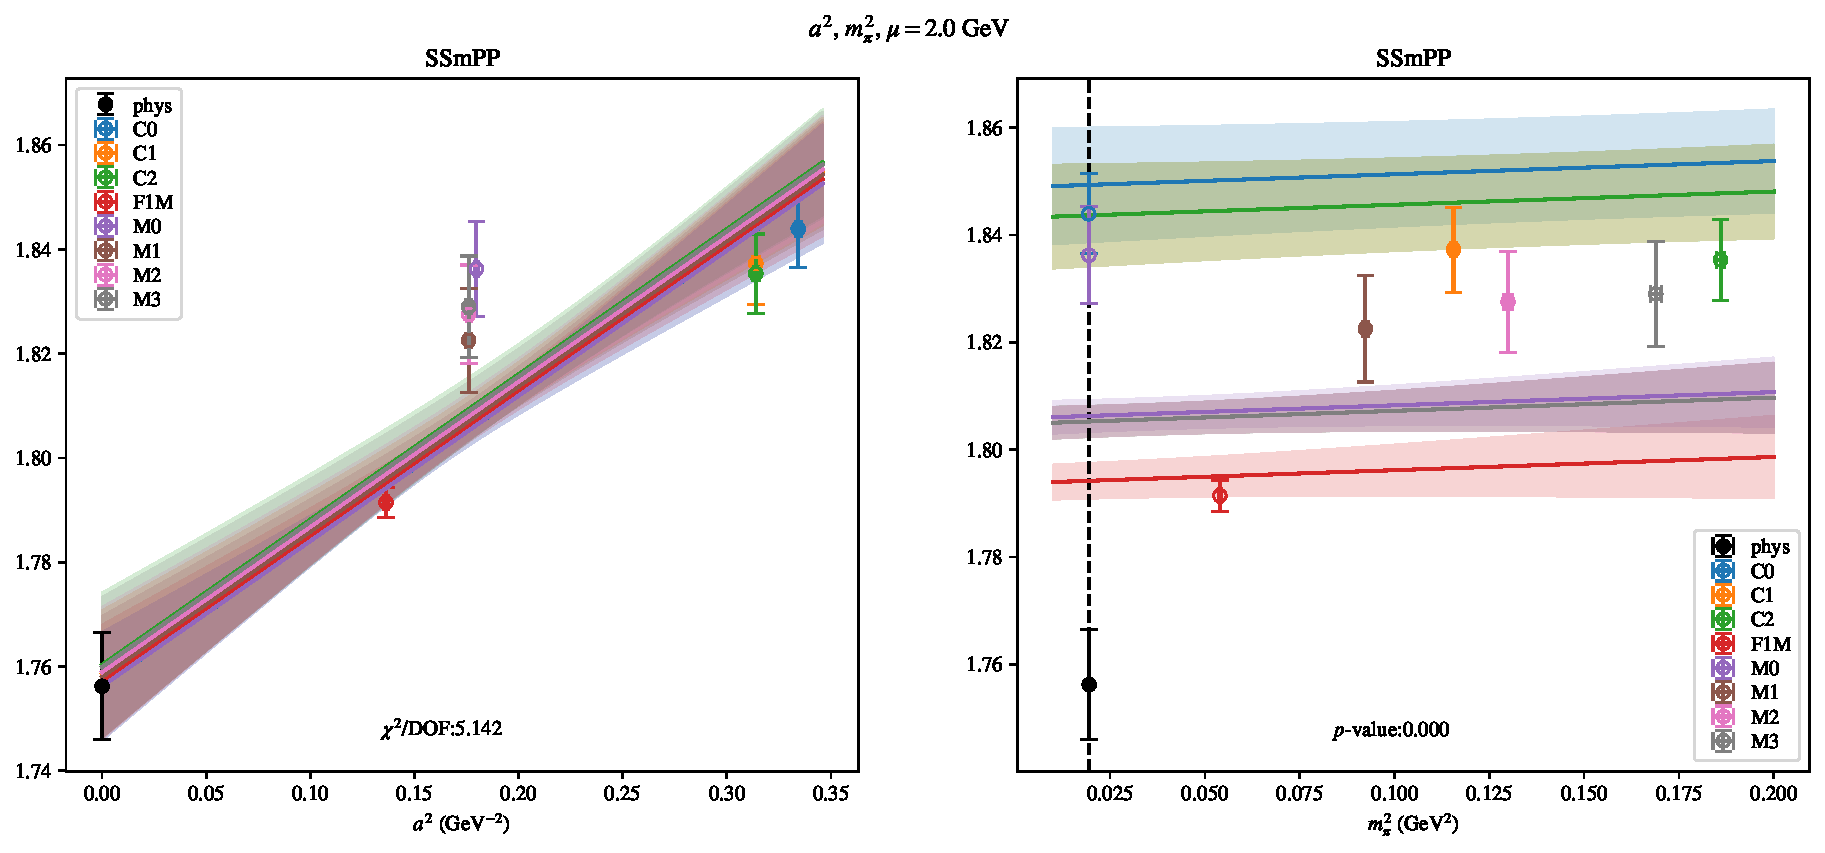
\includepdf[link, pages=-]{SSmPP/NPR/a2m2_20.pdf}
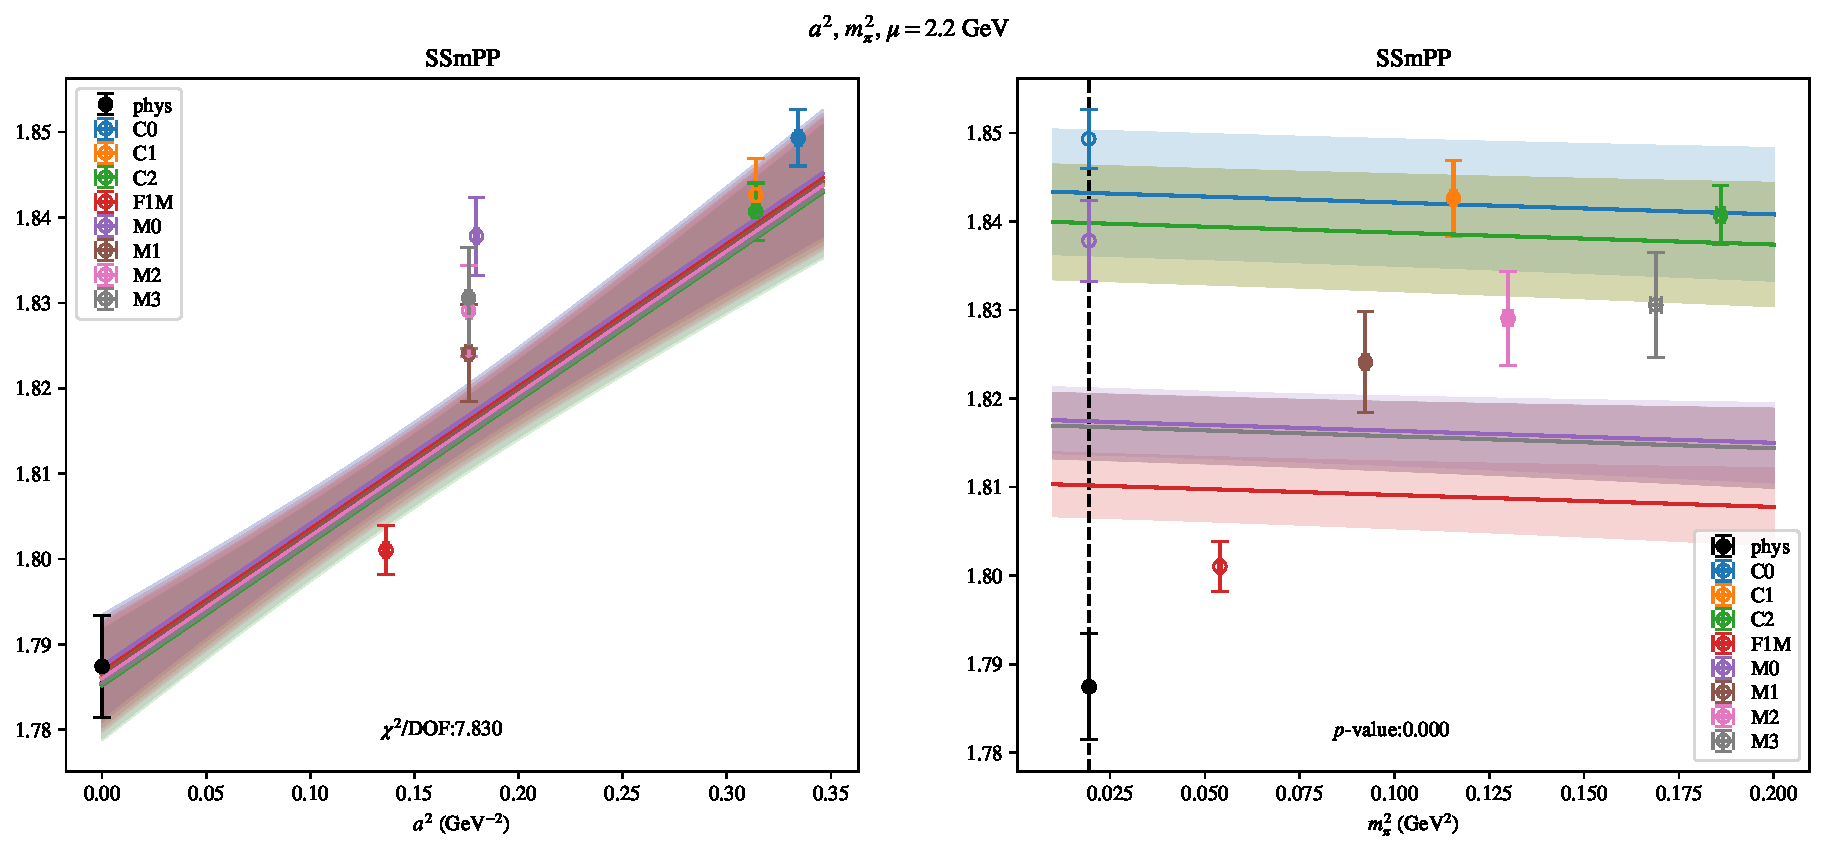
\includepdf[link, pages=-]{SSmPP/NPR/a2m2_22.pdf}
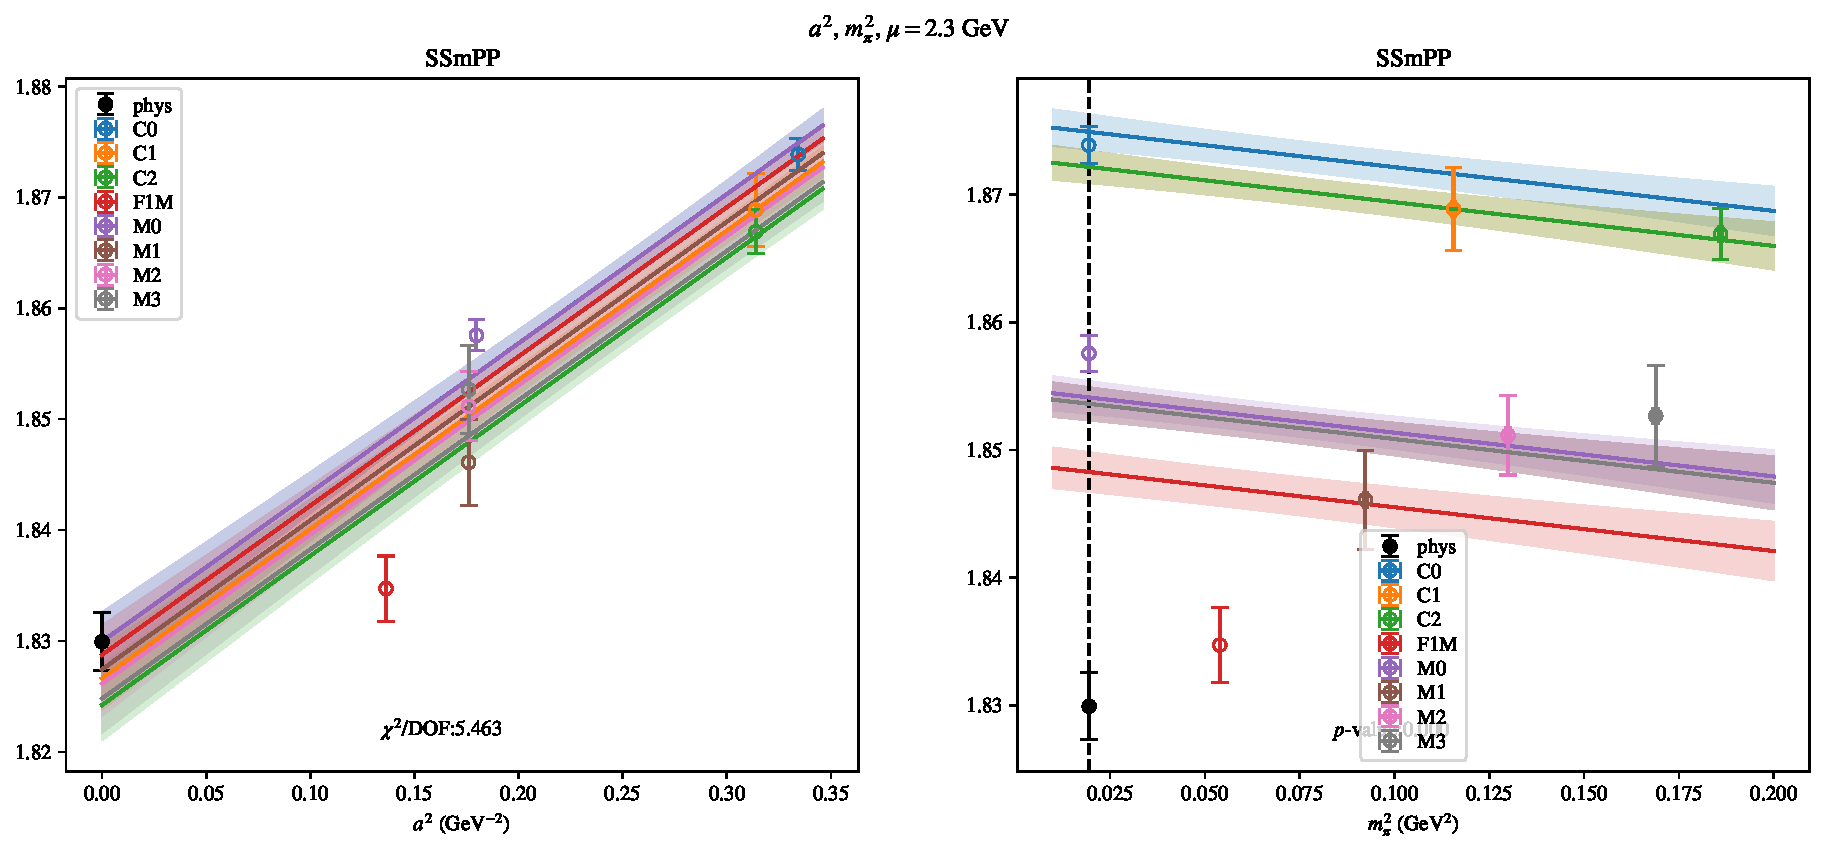
\includepdf[link, pages=-]{SSmPP/NPR/a2m2_23.pdf}
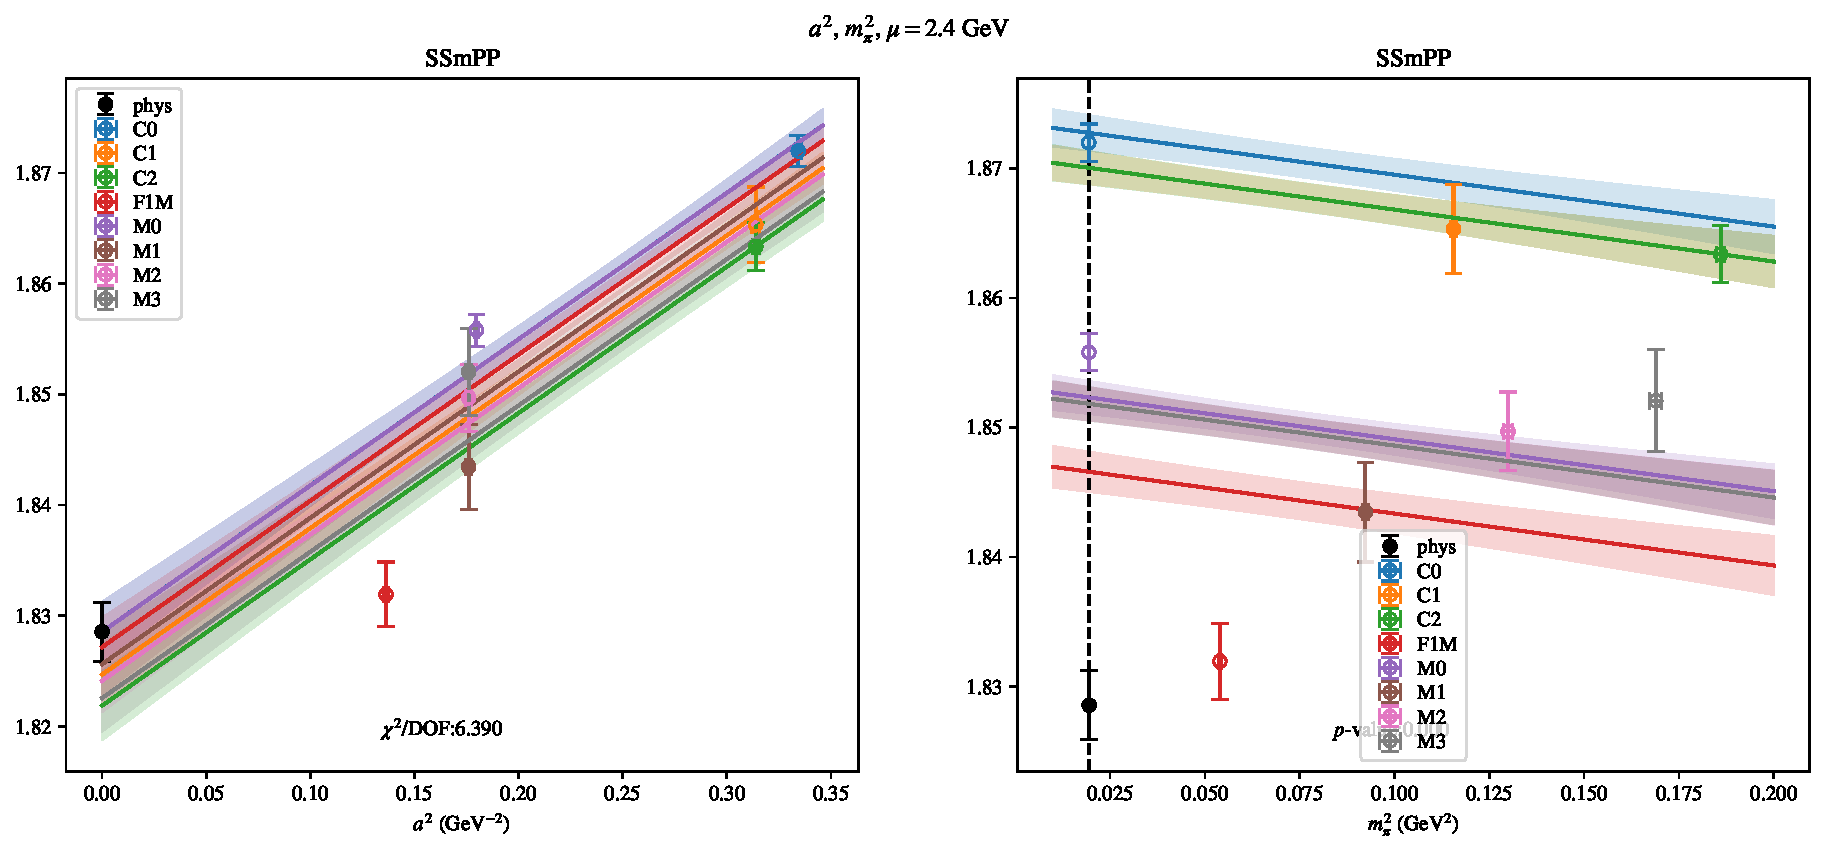
\includepdf[link, pages=-]{SSmPP/NPR/a2m2_24.pdf}
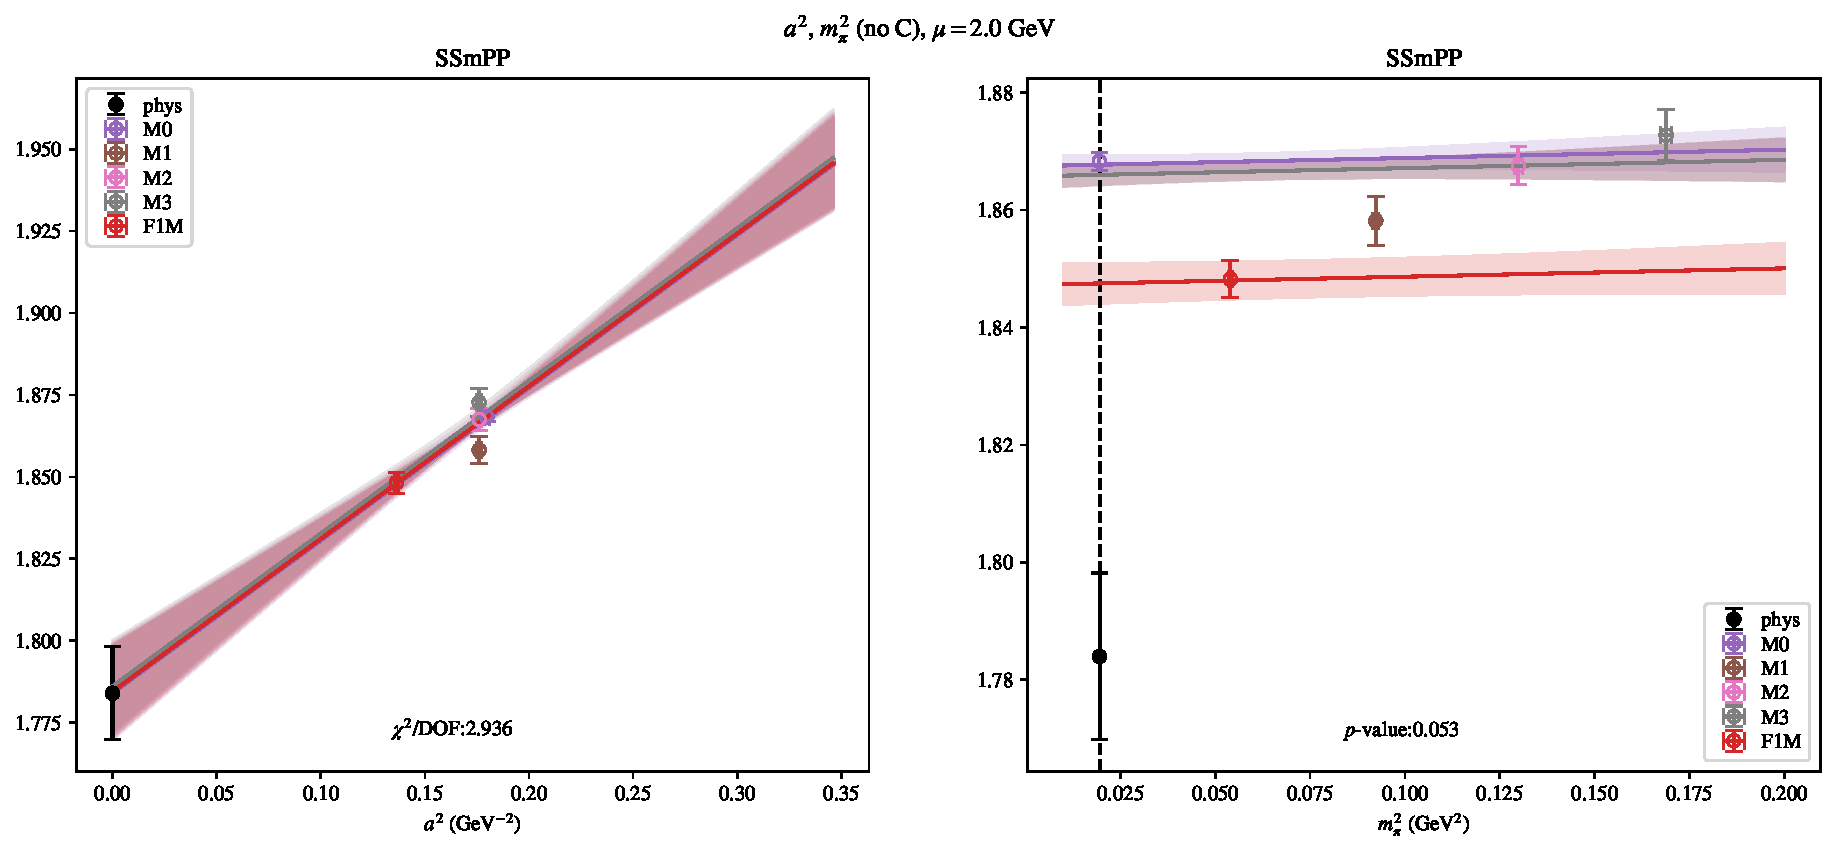
\includepdf[link, pages=-]{SSmPP/NPR/a2m2noC_20.pdf}
\includepdf[link, pages=-]{SSmPP/NPR/a2m2noC_22.pdf}
\includepdf[link, pages=-]{SSmPP/NPR/a2m2noC_23.pdf}
\includepdf[link, pages=-]{SSmPP/NPR/a2m2noC_24.pdf}
\includepdf[link, pages=-]{SSmPP/NPR/a2a4m2_20.pdf}
\includepdf[link, pages=-]{SSmPP/NPR/a2a4m2_22.pdf}
\includepdf[link, pages=-]{SSmPP/NPR/a2a4m2_23.pdf}
\includepdf[link, pages=-]{SSmPP/NPR/a2a4m2_24.pdf}
\includepdf[link, pages=-]{SSmPP/NPR/a2m2mcut_20.pdf}
\includepdf[link, pages=-]{SSmPP/NPR/a2m2mcut_22.pdf}
\includepdf[link, pages=-]{SSmPP/NPR/a2m2mcut_23.pdf}
\includepdf[link, pages=-]{SSmPP/NPR/a2m2mcut_24.pdf}
\includepdf[link, pages=-]{SSmPP/NPR/a2m2m4_20.pdf}
\includepdf[link, pages=-]{SSmPP/NPR/a2m2m4_22.pdf}
\includepdf[link, pages=-]{SSmPP/NPR/a2m2m4_23.pdf}
\includepdf[link, pages=-]{SSmPP/NPR/a2m2m4_24.pdf}
\clearpage
\section{$\mathcal{B}_4$}
\begin{table}[h!]
\begin{center}
\begin{tabular}{|c|c|c|c|c|c|}
\hline
$\mu$ (GeV) & $a^2$, $m_\pi^2$& $a^2$, $m_\pi^2$ (no C)& $a^2$, $a^4$, $m_\pi^2$& $a^2$, $m_\pi^2$ (no M3, C2)& $a^2$, $m_\pi^2$, $m_\pi^4$\\
\hline
2.0& \hyperlink{SSpPP/NPR/a2m2_20.pdf.1}{\textbf{-1(14)}: 19321.357 (0.0)} & \hyperlink{SSpPP/NPR/a2m2noC_20.pdf.1}{\textbf{22(65)}: 26585.047 (0.0)} & \hyperlink{SSpPP/NPR/a2a4m2_20.pdf.1}{\textbf{-(13)}: 24104.429 (0.0)} & \hyperlink{SSpPP/NPR/a2m2mcut_20.pdf.1}{\textbf{-2(30)}: 14722.37 (0.0)} & \hyperlink{SSpPP/NPR/a2m2m4_20.pdf.1}{\textbf{-2(15)}: 4633.002 (0.0)}\\
2.2& \hyperlink{SSpPP/NPR/a2m2_22.pdf.1}{\textbf{-1(14)}: 19431.812 (0.0)} & \hyperlink{SSpPP/NPR/a2m2noC_22.pdf.1}{\textbf{21(64)}: 26747.963 (0.0)} & \hyperlink{SSpPP/NPR/a2a4m2_22.pdf.1}{\textbf{-(12)}: 24245.309 (0.0)} & \hyperlink{SSpPP/NPR/a2m2mcut_22.pdf.1}{\textbf{-1(29)}: 14867.319 (0.0)} & \hyperlink{SSpPP/NPR/a2m2m4_22.pdf.1}{\textbf{-2(15)}: 4691.512 (0.0)}\\
2.3& \hyperlink{SSpPP/NPR/a2m2_23.pdf.1}{\textbf{-1(14)}: 19470.107 (0.0)} & \hyperlink{SSpPP/NPR/a2m2noC_23.pdf.1}{\textbf{21(63)}: 26794.189 (0.0)} & \hyperlink{SSpPP/NPR/a2a4m2_23.pdf.1}{\textbf{-(12)}: 24294.592 (0.0)} & \hyperlink{SSpPP/NPR/a2m2mcut_23.pdf.1}{\textbf{-1(29)}: 14919.225 (0.0)} & \hyperlink{SSpPP/NPR/a2m2m4_23.pdf.1}{\textbf{-2(15)}: 4717.694 (0.0)}\\
2.4& \hyperlink{SSpPP/NPR/a2m2_24.pdf.1}{\textbf{-1(14)}: 19494.308 (0.0)} & \hyperlink{SSpPP/NPR/a2m2noC_24.pdf.1}{\textbf{21(62)}: 26842.422 (0.0)} & \hyperlink{SSpPP/NPR/a2a4m2_24.pdf.1}{\textbf{-(12)}: 24326.566 (0.0)} & \hyperlink{SSpPP/NPR/a2m2mcut_24.pdf.1}{\textbf{-1(28)}: 14959.564 (0.0)} & \hyperlink{SSpPP/NPR/a2m2m4_24.pdf.1}{\textbf{-2(14)}: 4734.91 (0.0)}\\
\hline
\end{tabular}
\caption{Physical point value from chiral and continuum extrapolation at renormalisation scale $\mu$. Entries are \textbf{value(error)}: $\chi^2/\text{DOF}$ ($p$-value).}
\end{center}
\end{table}
\begin{table}[h!]
\begin{center}
\begin{tabular}{|c c|c|c|c|c|c|}
\hline
$\mu$ (GeV) &  & $a^2$, $m_\pi^2$& $a^2$, $m_\pi^2$ (no C)& $a^2$, $a^4$, $m_\pi^2$& $a^2$, $m_\pi^2$ (no M3, C2)& $a^2$, $m_\pi^2$, $m_\pi^4$\\
\hline
\multirow{2}{0.5in}{2.0} & $\alpha$ & 3.199(86)& -10.(12)& -3.4(32)& 1.897(83)& 0.636(20)\\
 & $\beta$ & -0.162(21)& 0.0841(24)& -0.072(46)& -0.205(29)& -0.341(19)\\
\hline
\multirow{2}{0.5in}{2.2} & $\alpha$ & 3.228(86)& -10.(12)& -3.3(34)& 1.918(84)& 0.645(20)\\
 & $\beta$ & -0.163(22)& 0.0838(23)& -0.074(48)& -0.205(29)& -0.342(19)\\
\hline
\multirow{2}{0.5in}{2.3} & $\alpha$ & 3.243(87)& -10.(12)& -3.2(34)& 1.929(84)& 0.650(20)\\
 & $\beta$ & -0.163(22)& 0.0837(23)& -0.075(49)& -0.206(29)& -0.342(19)\\
\hline
\multirow{2}{0.5in}{2.4} & $\alpha$ & 3.262(87)& -10.(12)& -3.2(35)& 1.941(84)& 0.656(20)\\
 & $\beta$ & -0.164(22)& 0.0836(23)& -0.076(50)& -0.206(29)& -0.343(19)\\
\hline
\end{tabular}
\caption{Fit values of coefficients in $Q = Q_{phys} + \mathbf{\alpha} a^2 + \mathbf{\beta}\left(\frac{m_\pi^2}{f_\pi^2}-\frac{m_{\pi,PDG}^2}{f_\pi^2}\right) + \ldots$.}
\end{center}
\end{table}
\includepdf[link, pages=-]{SSpPP/NPR/a2m2_20.pdf}
\includepdf[link, pages=-]{SSpPP/NPR/a2m2_22.pdf}
\includepdf[link, pages=-]{SSpPP/NPR/a2m2_23.pdf}
\includepdf[link, pages=-]{SSpPP/NPR/a2m2_24.pdf}
\includepdf[link, pages=-]{SSpPP/NPR/a2m2noC_20.pdf}
\includepdf[link, pages=-]{SSpPP/NPR/a2m2noC_22.pdf}
\includepdf[link, pages=-]{SSpPP/NPR/a2m2noC_23.pdf}
\includepdf[link, pages=-]{SSpPP/NPR/a2m2noC_24.pdf}
\includepdf[link, pages=-]{SSpPP/NPR/a2a4m2_20.pdf}
\includepdf[link, pages=-]{SSpPP/NPR/a2a4m2_22.pdf}
\includepdf[link, pages=-]{SSpPP/NPR/a2a4m2_23.pdf}
\includepdf[link, pages=-]{SSpPP/NPR/a2a4m2_24.pdf}
\includepdf[link, pages=-]{SSpPP/NPR/a2m2mcut_20.pdf}
\includepdf[link, pages=-]{SSpPP/NPR/a2m2mcut_22.pdf}
\includepdf[link, pages=-]{SSpPP/NPR/a2m2mcut_23.pdf}
\includepdf[link, pages=-]{SSpPP/NPR/a2m2mcut_24.pdf}
\includepdf[link, pages=-]{SSpPP/NPR/a2m2m4_20.pdf}
\includepdf[link, pages=-]{SSpPP/NPR/a2m2m4_22.pdf}
\includepdf[link, pages=-]{SSpPP/NPR/a2m2m4_23.pdf}
\includepdf[link, pages=-]{SSpPP/NPR/a2m2m4_24.pdf}
\clearpage
\section{$\mathcal{B}_5$}
\begin{table}[h!]
\begin{center}
\begin{tabular}{|c|c|c|c|c|c|}
\hline
$\mu$ (GeV) & $a^2$, $m_\pi^2$& $a^2$, $m_\pi^2$ (no C)& $a^2$, $a^4$, $m_\pi^2$& $a^2$, $m_\pi^2$ (no M3, C2)& $a^2$, $m_\pi^2$, $m_\pi^4$\\
\hline
2.0& \hyperlink{TT/NPR/a2m2_20.pdf.1}{\textbf{-45(55)}: 17096.455 (0.0)} & \hyperlink{TT/NPR/a2m2noC_20.pdf.1}{\textbf{85(25)}: 23134.53 (0.0)} & \hyperlink{TT/NPR/a2a4m2_20.pdf.1}{\textbf{-1(51)}: 21262.08 (0.0)} & \hyperlink{TT/NPR/a2m2mcut_20.pdf.1}{\textbf{-7(11)}: 12246.406 (0.0)} & \hyperlink{TT/NPR/a2m2m4_20.pdf.1}{\textbf{-10(60)}: 3655.794 (0.0)}\\
2.2& \hyperlink{TT/NPR/a2m2_22.pdf.1}{\textbf{-45(53)}: 18096.113 (0.0)} & \hyperlink{TT/NPR/a2m2noC_22.pdf.1}{\textbf{85(24)}: 24856.421 (0.0)} & \hyperlink{TT/NPR/a2a4m2_22.pdf.1}{\textbf{-1(50)}: 22519.23 (0.0)} & \hyperlink{TT/NPR/a2m2mcut_22.pdf.1}{\textbf{-7(10)}: 12959.163 (0.0)} & \hyperlink{TT/NPR/a2m2m4_22.pdf.1}{\textbf{-10(57)}: 3819.876 (0.0)}\\
2.3& \hyperlink{TT/NPR/a2m2_23.pdf.1}{\textbf{-44(52)}: 18351.48 (0.0)} & \hyperlink{TT/NPR/a2m2noC_23.pdf.1}{\textbf{85(24)}: 25228.853 (0.0)} & \hyperlink{TT/NPR/a2a4m2_23.pdf.1}{\textbf{-1(49)}: 22841.031 (0.0)} & \hyperlink{TT/NPR/a2m2mcut_23.pdf.1}{\textbf{-7(10)}: 13074.692 (0.0)} & \hyperlink{TT/NPR/a2m2m4_23.pdf.1}{\textbf{-10(56)}: 3844.174 (0.0)}\\
2.4& \hyperlink{TT/NPR/a2m2_24.pdf.1}{\textbf{-44(52)}: 18521.422 (0.0)} & \hyperlink{TT/NPR/a2m2noC_24.pdf.1}{\textbf{84(24)}: 25482.221 (0.0)} & \hyperlink{TT/NPR/a2a4m2_24.pdf.1}{\textbf{-1(49)}: 23055.41 (0.0)} & \hyperlink{TT/NPR/a2m2mcut_24.pdf.1}{\textbf{-7(10)}: 13138.571 (0.0)} & \hyperlink{TT/NPR/a2m2m4_24.pdf.1}{\textbf{-10(55)}: 3851.878 (0.0)}\\
\hline
\end{tabular}
\caption{Physical point value from chiral and continuum extrapolation at renormalisation scale $\mu$. Entries are \textbf{value(error)}: $\chi^2/\text{DOF}$ ($p$-value).}
\end{center}
\end{table}
\begin{table}[h!]
\begin{center}
\begin{tabular}{|c c|c|c|c|c|c|}
\hline
$\mu$ (GeV) &  & $a^2$, $m_\pi^2$& $a^2$, $m_\pi^2$ (no C)& $a^2$, $a^4$, $m_\pi^2$& $a^2$, $m_\pi^2$ (no M3, C2)& $a^2$, $m_\pi^2$, $m_\pi^4$\\
\hline
\multirow{2}{0.5in}{2.0} & $\alpha$ & 2.528(74)& -10.(12)& -4.9(17)& 1.568(77)& 0.529(20)\\
 & $\beta$ & -0.149(19)& 0.0792(24)& -0.050(24)& -0.197(27)& -0.334(19)\\
\hline
\multirow{2}{0.5in}{2.2} & $\alpha$ & 2.446(71)& -10.(12)& -4.8(18)& 1.528(75)& 0.506(20)\\
 & $\beta$ & -0.147(18)& 0.0779(23)& -0.052(26)& -0.195(27)& -0.333(18)\\
\hline
\multirow{2}{0.5in}{2.3} & $\alpha$ & 2.412(71)& -10.(11)& -4.7(19)& 1.510(75)& 0.498(19)\\
 & $\beta$ & -0.147(18)& 0.0776(23)& -0.053(26)& -0.195(27)& -0.332(18)\\
\hline
\multirow{2}{0.5in}{2.4} & $\alpha$ & 2.381(70)& -10.(11)& -4.7(19)& 1.492(74)& 0.491(19)\\
 & $\beta$ & -0.146(18)& 0.0775(22)& -0.053(27)& -0.194(26)& -0.332(18)\\
\hline
\end{tabular}
\caption{Fit values of coefficients in $Q = Q_{phys} + \mathbf{\alpha} a^2 + \mathbf{\beta}\left(\frac{m_\pi^2}{f_\pi^2}-\frac{m_{\pi,PDG}^2}{f_\pi^2}\right) + \ldots$.}
\end{center}
\end{table}
\includepdf[link, pages=-]{TT/NPR/a2m2_20.pdf}
\includepdf[link, pages=-]{TT/NPR/a2m2_22.pdf}
\includepdf[link, pages=-]{TT/NPR/a2m2_23.pdf}
\includepdf[link, pages=-]{TT/NPR/a2m2_24.pdf}
\includepdf[link, pages=-]{TT/NPR/a2m2noC_20.pdf}
\includepdf[link, pages=-]{TT/NPR/a2m2noC_22.pdf}
\includepdf[link, pages=-]{TT/NPR/a2m2noC_23.pdf}
\includepdf[link, pages=-]{TT/NPR/a2m2noC_24.pdf}
\includepdf[link, pages=-]{TT/NPR/a2a4m2_20.pdf}
\includepdf[link, pages=-]{TT/NPR/a2a4m2_22.pdf}
\includepdf[link, pages=-]{TT/NPR/a2a4m2_23.pdf}
\includepdf[link, pages=-]{TT/NPR/a2a4m2_24.pdf}
\includepdf[link, pages=-]{TT/NPR/a2m2mcut_20.pdf}
\includepdf[link, pages=-]{TT/NPR/a2m2mcut_22.pdf}
\includepdf[link, pages=-]{TT/NPR/a2m2mcut_23.pdf}
\includepdf[link, pages=-]{TT/NPR/a2m2mcut_24.pdf}
\includepdf[link, pages=-]{TT/NPR/a2m2m4_20.pdf}
\includepdf[link, pages=-]{TT/NPR/a2m2m4_22.pdf}
\includepdf[link, pages=-]{TT/NPR/a2m2m4_23.pdf}
\includepdf[link, pages=-]{TT/NPR/a2m2m4_24.pdf}
\clearpage
\end{document}